\documentclass{report}
\usepackage{float}
\usepackage{graphicx} % Required for inserting images
%\usepackage{amsmath}
\usepackage{physics}
%\usepackage{asymptote}
\usepackage{amssymb}
%\usepackage{kmath,kerkis} % The order of the packages matters; kmath changes the default text font
%\usepackage{mathabx}
\DeclareMathOperator{\proj}{proj}
\usepackage{bm}
\usepackage[vmargin=1in, hmargin=1in]{geometry}
\usepackage{mathrsfs}
\usepackage{fontspec}
\usepackage{tikz}
\usetikzlibrary{positioning, quotes, angles, decorations.pathreplacing, calc, arrows.meta}
\usepackage{physics}
\renewcommand{\figurename}{Fig.}
\usepackage{chngcntr}
\usepackage{tikz-3dplot}
\usepackage{caption}
\let\div\relax
\setlength{\captionmargin}{0pt}
%\captionsetup{singlelinecheck=false,justification=raggedright,font=footnotesize}
\usepackage{subcaption}
\usepackage{cancel}
\numberwithin{equation}{section}
\usetikzlibrary{quotes,angles}
\newcommand{\pd}[2]{\frac{\partial #1}{\partial #2}}
\newcommand{\pdd}[2]{\frac{\partial^2 #1}{\partial #2^2}}
\newcommand{\pds}[3]{\frac{\partial^ #3 #1}{\partial #2^#3}}
\newcommand{\limz}[1]{\lim_{#1\rightarrow 0}}
\counterwithin{figure}{section}
\title{Physics 4B Lecture Notes}
\author{Ryan Safarha}
\date{}

\begin{document}
\maketitle
\tableofcontents
\newpage
\chapter{Oscillations and Waves}
\section{Lecture 1}
\subsection{Simple Harmonic Oscillators}
Recall that for a horizontal mass-spring system, the equation of motion is given by Hooke's Law
\begin{equation}
	\ddot{x} = -\frac{k}{m}x
\end{equation}
This differential equation has the solution
\begin{equation}
	x(t) = A\cos(\omega t) + B\sin(\omega t) = C\cos(\omega t + \phi)
\end{equation}
The force $F =-kx$ is derived from the potential $U = \frac{1}{2}kx^2$. If you have a more general $U(x)$, and do a Taylor expansion on it
\begin{equation}
	U(x) = U(x_0) + U'(x_0)(x-x_0) + U''(x_0)\frac{(x-x_0)^2}{2}+O(x-x_0)^3
\end{equation}
If $x_0$ is centred around a minimum, the second term vanishes. We can also neglect the higher order terms, and we get the desired result. Using complex exponentials, we can write
\begin{equation}
	x(t) = Ae^{i\omega t}
\end{equation}
This is a linear equation, so we can take the real part to deal with the physics. It follows from (1.4) that
\begin{align*}
	\dot{x} = i\omega Ae^{i\omega t}\\
	\ddot{x} = -\omega^2Ae^{i\omega t}
\end{align*}
Taking the real parts of the above give us
\begin{align*}
	x(t) = A\cos(\omega t)\\
	\dot{x} = -A\omega \sin(\omega t)
\end{align*}
\subsection{Damped oscillations}
This is given by the equation
\begin{equation}
	\ddot{x} + \gamma \dot{x} +\frac{k}{m}x =0
\end{equation}
We can guess a solution of the form
\begin{equation}
	x(t) = Ae^{\alpha t}
\end{equation}
Plugging (1.6) into (1.5) we get
\begin{equation}
	\alpha^2 + \alpha \gamma + \omega_0^2 = 0
\end{equation}
Where
\begin{equation}
	\omega_0 = \sqrt{\frac{k}{m}}
\end{equation}
From the quadratic equation (1.7), we solve and get
\begin{equation}
	\alpha = -\frac{\gamma}{2}\pm \sqrt{\frac{\gamma ^2}{4} -\omega_0^2}
\end{equation}
You can see we have two solutions $(\alpha_-, \alpha_+)$. By superposition, our general solution is
\begin{equation}
	x(t) = Ae^{\alpha_+t}+Be^{\alpha_-t}
\end{equation}
When $\frac{\gamma}{2} > \omega_0$, we get \textbf{overdamping}. Otherwise (negating the equality), we get \textbf{underdamping}.
\begin{equation}
	\alpha_{+/-} = -\frac{\gamma}{2} \pm i\sqrt{\omega_0^2-\frac{\gamma^2}{4}} = -\frac{\gamma}{2} \pm i\omega'
\end{equation}
We can with this write our general solution
\begin{equation}
	x(t) = e^{-\frac{\gamma}{2}t}\left[Ae^{i\omega' t} + B e^{-i\omega't}\right] = Ce^{-\frac{\gamma}{2}t}\cos(\omega't +\phi)
\end{equation}
Looking at the case where $\frac{\gamma}{2} = \omega_0$ (critical damping), we get the general solution
\begin{equation}
	x(t) = Ae^{-\frac{\gamma}{2}t} + Bte^{-\frac{\gamma}{2}t}
\end{equation}

\begin{figure}[H]
\centering
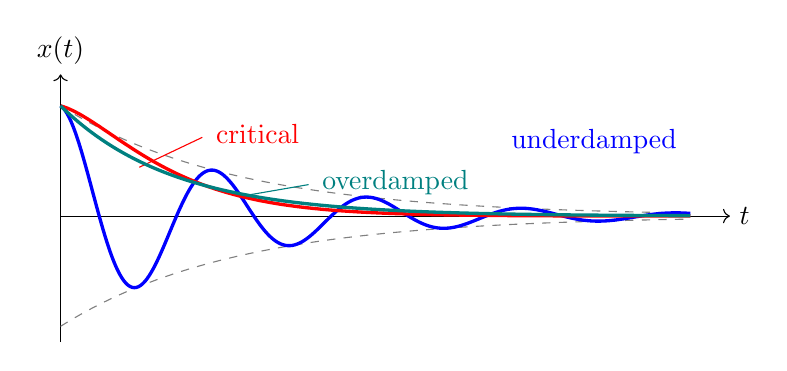
\begin{tikzpicture}[scale=1.0]
    % axes
    \draw[->] (0,0) -- (8.5,0) node[right] {$t$};
    \draw[->] (0,-1.6) -- (0,1.8) node[above] {$x(t)$};

    % underdamped: oscillation inside decaying envelope
    \draw[gray, dashed, domain=0:8, samples=100]
        plot (\x, {1.4*exp(-0.45*\x)});
    \draw[gray, dashed, domain=0:8, samples=100]
        plot (\x, {-1.4*exp(-0.45*\x)});
    \draw[blue, very thick, domain=0:8, samples=300]
        plot (\x, {1.4*exp(-0.45*\x)*cos(deg(3.2*\x))});
    \node[blue, right] at (5.6, 0.95) {underdamped};

    % critically damped
    \draw[red, very thick, domain=0:8, samples=200]
        plot (\x, {1.4*(1+1.1*\x)*exp(-1.3*\x)});
    \node[red, right] at (1.85, 1.05) {critical};
    \draw[red] (1.8,1.0) -- (1.0,0.62);

    % overdamped
    \draw[teal, very thick, domain=0:8, samples=200]
        plot (\x, {1.4*exp(-0.7*\x)});
    \node[teal, right] at (3.2, 0.42) {overdamped};
    \draw[teal] (3.15,0.40) -- (2.4,0.27);
\end{tikzpicture}
\caption{The three damping regimes. Underdamped motion oscillates within a
decaying exponential envelope (dashed); critically damped motion returns to
equilibrium fastest without oscillating; overdamped motion returns slowly.}
\label{fig:damping_regimes}
\end{figure}

\paragraph{Critical damping solution.}
At critical damping the characteristic equation $\alpha^2+\gamma\alpha+\omega_0^2=0$
has a repeated root $\alpha=-\gamma/2$ (since the discriminant
$\gamma^2/4-\omega_0^2=0$). A repeated root yields only one independent
exponential solution $e^{-\gamma t/2}$; the second independent solution of a
linear ODE with a repeated root is obtained by multiplying by $t$, giving
$te^{-\gamma t/2}$. One verifies directly: with $x=te^{-\gamma t/2}$,
$\dot x=(1-\tfrac{\gamma}{2}t)e^{-\gamma t/2}$ and
$\ddot x=(-\gamma+\tfrac{\gamma^2}{4}t)e^{-\gamma t/2}$, so
$\ddot x+\gamma\dot x+\tfrac{\gamma^2}{4}x
=(-\gamma+\gamma)e^{-\gamma t/2}+(\tfrac{\gamma^2}{4}-\tfrac{\gamma^2}{2}+\tfrac{\gamma^2}{4})te^{-\gamma t/2}=0$,
as required. Hence (1.13).
\subsection{Driven Oscillations}
This is given by the equation
\begin{equation}
	\ddot{x} + \gamma \dot{x} +\frac{k}{m}x = \frac{F_0}{m}\cos(\omega t)
\end{equation}
Note we're assuming a sinusoidal external force. Note the difference between $\omega$ and $\omega_0$, where the former is the frequency of the driving force and the latter is the natural frequency of the system without the driving force. We can write the driving force into a complex exponential form
\begin{equation}
		\ddot{z} + \gamma \dot{z} +\frac{k}{m}z = \frac{F_0}{m}e^{i\omega t}
\end{equation}
We've changed to $z$ since now our differential equation has a complex part.
\begin{equation}
	z(t) = z_0e^{i\omega t}
\end{equation}
Where $z_0$ is also complex. The magnitude of the amplitude $z_0$ depends on $\omega$ in the following way, with the peak approximately at $\omega_0$ (when gamma is very small). This is known as resonance.

\begin{figure}[H]
\centering
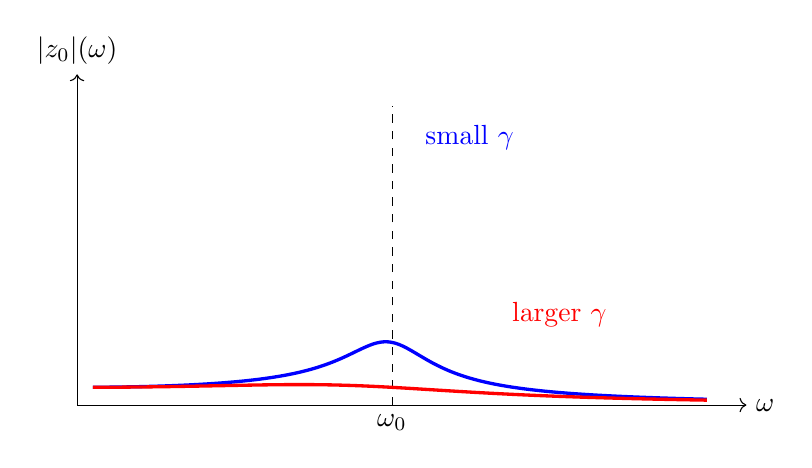
\begin{tikzpicture}[scale=1.0]
    % axes
    \draw[->] (0,0) -- (8.5,0) node[right] {$\omega$};
    \draw[->] (0,0) -- (0,4.2) node[above] {$|z_0|(\omega)$};
    \node[below] at (4.0,0) {$\omega_0$};
    \draw[dashed] (4.0,0) -- (4.0,3.8);

    % small gamma: sharp tall peak
    \draw[blue, very thick, domain=0.2:8, samples=300]
        plot (\x, {0.45/sqrt( (16-\x*\x)*(16-\x*\x)/64 + 0.02*\x*\x )});
    \node[blue, right] at (4.3,3.4) {small $\gamma$};

    % larger gamma: broad short peak
    \draw[red, very thick, domain=0.2:8, samples=300]
        plot (\x, {0.45/sqrt( (16-\x*\x)*(16-\x*\x)/64 + 0.25*\x*\x )});
    \node[red, right] at (5.4,1.15) {larger $\gamma$};
\end{tikzpicture}
\caption{Resonance: the steady-state amplitude $|z_0|$ as a function of the
driving frequency $\omega$. The response peaks near the natural frequency
$\omega_0$; smaller damping $\gamma$ gives a sharper, taller peak.}
\label{fig:resonance}
\end{figure}
\subsection{Waves}
We deal with transverse and longitudinal waves, which are classified based on how the particle is moving and the wave is moving. In a transverse wave, the particle moves perpendicular to the direction the wave moves. In a longitudinal wave, the particle moves parallel to the direction of the wave.

\begin{figure}[H]
\centering
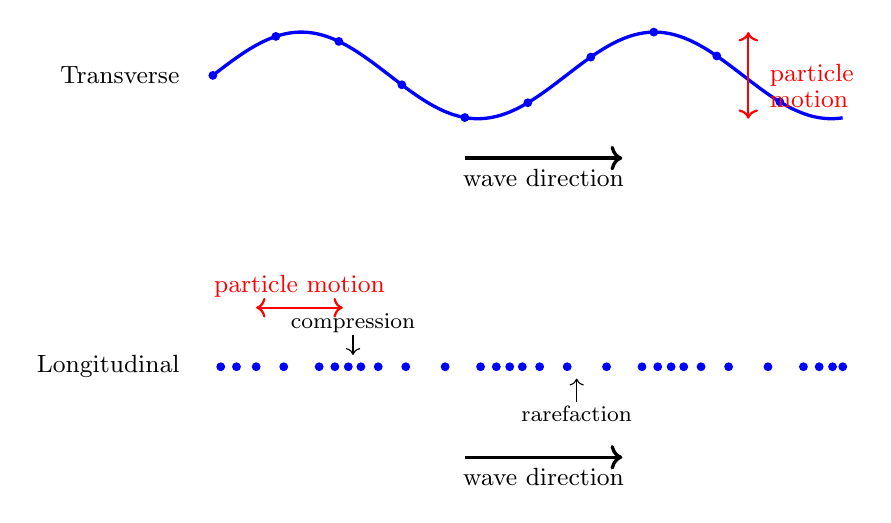
\begin{tikzpicture}[scale=1.0]

    % ;- Transverse wave (top) ;-
    \node[left, font=\small] at (-0.3, 1.6) {Transverse};
    % the wave shape
    \draw[blue, very thick, domain=0:8, samples=200]
        plot (\x, {1.6 + 0.55*sin(deg(1.4*\x))});
    % particle markers along the wave
    \foreach \x in {0,0.8,...,8}{
        \fill[blue] (\x, {1.6 + 0.55*sin(deg(1.4*\x))}) circle (1.6pt);
    }
    % propagation direction
    \draw[->, very thick] (3.2,0.55) -- (5.2,0.55)
        node[midway, below, font=\small] {wave direction};
    % particle motion arrow (perpendicular) - placed at a trough region
    \draw[<->, thick, red] (6.8,1.05) -- (6.8,2.15);
    \node[red, font=\small, right] at (6.95,1.60) {particle};
    \node[red, font=\small, right] at (6.95,1.30) {motion};

    % ;- Longitudinal wave (bottom) ;-
    \node[left, font=\small] at (-0.3, -2.1) {Longitudinal};
    % rows of dots with varying density (compressions and rarefactions)
    \foreach \x in {0.10,0.30,0.55,0.90,1.35,1.55,1.72,1.88,2.10,2.45,
                    2.95,3.40,3.60,3.77,3.93,4.15,4.50,5.00,5.45,5.65,
                    5.82,5.98,6.20,6.55,7.05,7.50,7.70,7.87,8.00}{
        \fill[blue] (\x,-2.1) circle (1.6pt);
    }
    % compression / rarefaction labels
    \node[font=\footnotesize] at (1.78,-1.55) {compression};
    \draw[->] (1.78,-1.7) -- (1.78,-1.95);
    \node[font=\footnotesize] at (4.62,-2.7) {rarefaction};
    \draw[->] (4.62,-2.55) -- (4.62,-2.25);
    % propagation direction
    \draw[->, very thick] (3.2,-3.25) -- (5.2,-3.25)
        node[midway, below, font=\small] {wave direction};
    % particle motion arrow (parallel)
    \draw[<->, thick, red] (0.55,-1.35) -- (1.65,-1.35)
        node[above, font=\small, midway] {particle motion};

\end{tikzpicture}
\caption{Transverse versus longitudinal waves. In a transverse wave the
particles oscillate perpendicular to the propagation direction; in a
longitudinal wave they oscillate along it, producing alternating
compressions and rarefactions.}
\label{fig:transverse_longitudinal}
\end{figure}
\section{Lecture 2}
\subsection{The equation for a travelling wave}
\begin{equation}
	\psi(x,t) = A\cos(kx-\omega t)
\end{equation}
Where $k$ is the \textbf{wave number} (units 1/m) and $\omega$ is the \textbf{angular frequency}. $k$ is related to the wavelength by the following
\begin{equation}
	k = \frac{2\pi}{\lambda}
\end{equation}
Similarly,
\begin{equation}
	\omega = \frac{2\pi}{T} = 2\pi f
\end{equation}
The velocity of the travelling wave is given by
\begin{equation}
	v = \frac{\lambda}{T} = \frac{\omega}{k}
\end{equation}
This follows from rewriting the wave equation as follows
\begin{align*}
	\psi(x,t) &= A\cos\!\left(k\left(x-\frac{\omega t}{k}\right)\right)\\
	\Rightarrow x &= \frac{\omega}{k}t + \phi
\end{align*}
Where $\phi$ is just some constant phase. This wave moves to the right. If we wanted one that would move to the left, we write
\begin{equation}
	\psi = A\cos(kx + \omega t)
\end{equation}
\subsection{The wave equation for a string}
Let's say the string is tied/held on both ends and there is a wave propagating through its length. We choose an arbitrary position on the wave at $x$ and draw a tangent to it. Then the angle of the tangent w.r.t the horizontal is $\theta(x)$. This is at $\psi(x,t)$. We move on to another point close to the first, given at $x+dx$ and $\theta(x+dx)$. This string has a tension $T$ with mass per unit length $\mu$. Apply Newton's second law to the piece of string between $x$ and $x+dx$. From the image you can see that the vertical components of the tension at the two points point in different directions. N2L gives
\begin{equation*}
	T\sin\theta(x + dx) - T\sin\theta(x) = \mu \,dx\,\frac{\partial^2\psi}{\partial t^2}
\end{equation*}
Assuming small angles, $\sin\theta \approx \tan\theta \approx \theta$. But $\tan\theta$ is the slope, $\frac{\partial \psi(x,t)}{\partial x}$. Now,
\begin{align*}
	T\left(\frac{\partial \psi}{\partial x}\bigg|_{x+dx} - \frac{\partial \psi}{\partial x}\bigg|_{x}\right) &= T\frac{\partial^2\psi}{\partial x^2}dx = \mu\, dx\,\frac{\partial ^2 \psi}{\partial t^2}\\
	\Rightarrow \frac{\partial^2\psi}{\partial x^2} &= \frac{\mu}{T}\frac{\partial ^2\psi}{\partial t^2}
\end{align*}
Our final wave equation is
\begin{equation}
	\frac{\partial^2\psi}{\partial x^2} = \frac{1}{v^2}\frac{\partial^2\psi}{\partial t^2}
\end{equation}
Where $v= \sqrt{\frac{T}{\mu}}$. To see this, take the second derivatives of $\psi(x,t)$ w.r.t $x$ and $t$
\begin{align*}
	\frac{\partial^2\psi}{\partial x^2} &= -k^2A\cos(kx-\omega t)\\
	\frac{\partial^2\psi}{\partial t^2} &= -\omega^2 A\cos(kx - \omega t)\\
	\Rightarrow k^2 &= \frac{1}{v^2}\omega^2 \\
	\Rightarrow v^2 &= \frac{\omega^2}{k^2}
\end{align*}
Note that we have a second derivative of position and time. We usually say that if we have one derivative of time and two derivatives of space this equation does not describe a wave, but this is the case in the Schr\"odinger Equation. Note, we can write our wave equation in complex-exponential form
\begin{equation}
	\psi(x,t) = Ae^{i(kx-\omega t)}
\end{equation}
Again, since everything is linear, we can just take the real part of the above equation. The wave has a fixed velocity, but we can vary $k$ and $\omega$.
\section{Lecture 3}
\subsection{Waves Continued}
From the analysis above we see that the wave speed is constant, but this is not generally the case. A dispersive medium is one that changes the wave speed. We can define the \textbf{phase speed}
\begin{equation}
	v_p(k) = \frac{\omega(k)}{k}
\end{equation}
In a non-dispersive medium, $v_p$ is constant. Consider the following solution to the wave equation
\begin{equation}
	\psi(x,t) = f(kx-\omega t)
\end{equation}
where $f$ is some arbitrary function. This does solve the wave equation, because
\begin{align*}
	\frac{\partial^2\psi}{\partial x^2}& = k^2f''\\
	\frac{\partial^2\psi}{\partial t^2} &= \omega^2 f''
\end{align*}
Plugging it into the wave equation
\begin{align*}
	k^2f'' &= \frac{\omega^2}{v^2}f''\\
	\Rightarrow v&=\frac{\omega}{k}
\end{align*}
we see that this satisfies the equation.
\subsection{Fourier Analysis}
When a bunch of waves are superposed, we have to do this analysis to decompose the function into sines and cosines. Working on a finite interval, we expand in a discrete set of modes $k_n$:
\begin{equation}
	\psi(x) =\sum_{n} \left[A_n\cos(k_n x)+B_n\sin(k_n x)\right]
\end{equation}
Our coefficients $A_n$ and $B_n$ are given by the usual projection integrals
\begin{align}
\begin{split}
	A_n = \frac{2}{L}\int_0^L dx\,\psi\cos(k_n x)\\
	B_n = \frac{2}{L}\int_0^L dx\,\psi\sin(k_n x)
\end{split}
\end{align}
For a function defined on the whole line, the sum is replaced by an integral over a continuum of $k$, the \textbf{Fourier transform}:
\begin{equation}
	\psi(x) =\int^{\infty}_{-\infty} dk\left[A(k)\cos(kx)+B(k)\sin(kx)\right],
\end{equation}
and the prefactor in the inversion formula becomes $1/\pi$ rather than $2/L$.
\subsection{Standing Waves}
What happens if we superpose a wave moving (say to the right) with a wave moving in the opposite direction. We have two equations
\begin{align*}
	\psi_1(x,t) &= A\cos(kx-\omega t)\\
	\psi_2(x,t) &= A\cos(kx+\omega t)
\end{align*}
By superposition we add waves; here it is convenient to add $\psi_1$ and $(-\psi_2)$, which is itself a perfectly valid leftward-travelling wave:
\begin{align*}
	\psi_1-\psi_2 &= A\left(\cos(kx-\omega t) - \cos(kx+\omega t)\right)\\
	 &= 2A\sin(kx)\sin(\omega t)
\end{align*}
Where the last line follows from the cosine addition formulae. We assume the boundary conditions to be that the strings are fixed at the two ends. The condition a standing wave must satisfy is that
\begin{align}
	k_nL = n\pi &= \frac{2\pi}{\lambda_n}L\\
	\Rightarrow \lambda_n &= \frac{2L}{n}
\end{align}
\begin{figure}[H]
\centering
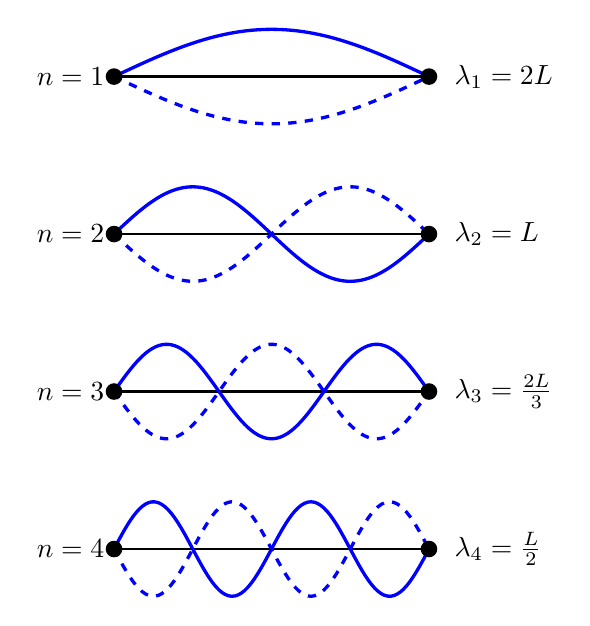
\begin{tikzpicture}[scale=1.0]

    % n=1 (fundamental)
    \node[left] at (0, 0) {$n=1$};
    \draw[thick] (0,0) -- (4,0); % axis
    \draw[blue, very thick, domain=0:4, samples=100]
        plot (\x, {0.6*sin(deg(\x*pi/4))});
    \draw[dashed, blue, very thick, domain=0:4, samples=100]
        plot (\x, {-0.6*sin(deg(\x*pi/4))});
    \fill (0,0) circle (3pt);
    \fill (4,0) circle (3pt);

    % n=2
    \node[left] at (0, -2) {$n=2$};
    \draw[thick] (0,-2) -- (4,-2);
    \draw[blue, very thick, domain=0:4, samples=100]
        plot (\x, {-2 + 0.6*sin(deg(\x*2*pi/4))});
    \draw[dashed, blue, very thick, domain=0:4, samples=100]
        plot (\x, {-2 - 0.6*sin(deg(\x*2*pi/4))});
    \fill (0,-2) circle (3pt);
    \fill (4,-2) circle (3pt);

    % n=3
    \node[left] at (0, -4) {$n=3$};
    \draw[thick] (0,-4) -- (4,-4);
    \draw[blue, very thick, domain=0:4, samples=100]
        plot (\x, {-4 + 0.6*sin(deg(\x*3*pi/4))});
    \draw[dashed, blue, very thick, domain=0:4, samples=100]
        plot (\x, {-4 - 0.6*sin(deg(\x*3*pi/4))});
    \fill (0,-4) circle (3pt);
    \fill (4,-4) circle (3pt);

    % n=4
    \node[left] at (0, -6) {$n=4$};
    \draw[thick] (0,-6) -- (4,-6);
    \draw[blue, very thick, domain=0:4, samples=100]
        plot (\x, {-6 + 0.6*sin(deg(\x*4*pi/4))});
    \draw[dashed, blue, very thick, domain=0:4, samples=100]
        plot (\x, {-6 - 0.6*sin(deg(\x*4*pi/4))});
    \fill (0,-6) circle (3pt);
    \fill (4,-6) circle (3pt);

    % Labels
    \node[right] at (4.2, 0)  {$\lambda_1 = 2L$};
    \node[right] at (4.2, -2) {$\lambda_2 = L$};
    \node[right] at (4.2, -4) {$\lambda_3 = \frac{2L}{3}$};
    \node[right] at (4.2, -6) {$\lambda_4 = \frac{L}{2}$};

\end{tikzpicture}
\caption{Standing waves at the first four harmonics}
\label{fig:standing_waves}
\end{figure}
Where $L$ is the length of the string, and $n$ is the normal mode index. From the above, we derive the following relations (assume the medium is non-dispersive)
\begin{align}
	\omega_n = k_n v &= \frac{n\pi v}{L}\\
	\Rightarrow f_n &= \frac{nv}{2L} = nf_1
\end{align}
Where the last line comes from the fact that $f_n = \frac{\omega_n}{2\pi}$, and $f_1$ is the first normal mode frequency. Now consider a wave fixed only at one end (say at $x=0$, with $x=L$ free). A fixed end is a node of $\psi$ and a free end is an antinode, so with these boundary conditions we again use
\begin{equation*}
	\psi = 2A\sin(kx)\sin(\omega t),
\end{equation*}
which already has a node at $x=0$. Requiring an antinode at $x=L$ (so that $\cos(k_nL)=\pm1$, i.e. $\sin(k_nL)=\pm1$) gives
\begin{equation}
	k_n = \left(n+\frac{1}{2}\right)\frac{\pi}{L}\hspace{0.3cm} n=0,1,\dots
\end{equation}
from $k=\frac{2\pi}{\lambda}$,
\begin{equation}
	\lambda_n = \frac{4L}{2n+1}
\end{equation}
and also,
\begin{equation}
	f_n = \frac{2n+1}{4L}v
\end{equation}
\subsection{Energy considerations}
Going back to propagating waves. Recall the velocity of the string is given by $\dot{\psi}(x,t)$. Say we shake a wave up and down, and it begins to oscillate up and down. To start, only a portion of the wave will be oscillating, but as the wave "reaches" the ends, the whole wave will oscillate. We are transferring energy into the wave without transferring mass. Let $dK$ be the differential kinetic energy
\begin{equation}
	dK = \frac{1}{2}\mu \,dx\left(\frac{\partial \psi}{\partial t}\right)^2
\end{equation}
Substituting our equation for a propagating wave
\begin{equation}
	u_K = \frac{dK}{dx} = \frac{1}{2}\mu A^2\omega^2\sin^2(kx-\omega t)
\end{equation}
Where the above is the kinetic energy per unit length. Moving on to potential energy. In our propagating wave, $dU = dK$, so we can write the total energy per unit length as
\begin{equation}
	u(x,t) = \mu A^2\omega^2\sin^2(kx-\omega t)
\end{equation}
The average of $\sin^2(\theta)$ over a period is $\frac{1}{2}$. This means the average energy per cycle per unit length is
\begin{equation}
	\bar{u} = \frac{1}{2}\mu A^2\omega^2
\end{equation}
Looking at potential energy, we have to consider something we neglected before, and this is what yields the $dU=dK$ equality. In vibrating the string, we stretch it a little, and so there is some potential energy stored in there. The reason the above equality holds is because the maximum stretch occurs also at the maximum speed. Quantitatively
\begin{align}
	dl &= \sqrt{dx^2 + d\psi^2} = dx\sqrt{1+\left(\frac{\partial\psi}{\partial x}\right)^2}\\
	&\approx dx\left(1+\frac{1}{2}\left(\frac{\partial \psi}{\partial x}\right)^2\right)
\end{align}
Where $dl$ is the elongation of the string. Then
\begin{align}
	\delta l = dl - dx &= \frac{1}{2}\left(\frac{\partial \psi}{\partial x}\right)^2 dx\\
	\Rightarrow \frac{dU}{dx} &= T\frac{\delta l}{dx} = \frac{1}{2}T\left(\frac{\partial \psi}{\partial x}\right)^2 = \frac{1}{2}Tk^2A^2\sin^2(kx-\omega t)
\end{align}
But $Tk^2 = \mu \omega^2$, so we get
\begin{equation}
dU = dK = \frac{1}{2}\mu A^2\omega^2\sin^2(kx-\omega t)
\end{equation}
as desired.
\section{Lecture 4}
\subsection{Energy of a wave continued}
Recall that we said the average energy per unit length $\bar{u}$ was given by
\begin{equation}
	\bar{u} = \frac{1}{2}\mu A^2\omega^2
\end{equation}
Where $\mu$ is the mass per unit length. In a time $dt$, the wave advances $dx$. So the change in energy
\begin{equation}
	dE = \bar{u}\,dx = \bar{u}\,v\,dt
\end{equation}
Then the energy per unit time (power), is given by
\begin{equation}
	P = \bar{u}\,v
\end{equation}
\subsection{3 Dimensions}
Take a sound wave, where the wave is propagating like a sphere. The area is spreading out. So in 3D, what is relevant is the power per unit area at that point.
\begin{equation}
	I = \frac{P}{4\pi r^2}
\end{equation}
Where $I$ is the intensity. The wave equation in three dimensions is given by
\begin{equation}
	\nabla^2\psi = \frac{1}{v^2}\frac{\partial^2\psi}{\partial t^2}
\end{equation}
Here $\psi = \psi(\textbf{r},t)$. We could use cartesian coordinates $\textbf{r} = (x,y,z)$ or spherical coordinates, where the position vector is simply $\textbf{r} = r\,\vu{r}$. For a spherically symmetric wave the only thing that matters is the radial component. Recall the Laplacian of $\psi$ in spherical coordinates (radial part) is given by
\begin{equation*}
	\nabla^2\psi = \frac{1}{r}\frac{\partial^2}{\partial r^2}(r\psi)
\end{equation*}
Then our 3D spherically symmetric wave equation is
\begin{equation}
	\frac{1}{r}\frac{\partial^2}{\partial r^2}(r\psi) =\frac{1}{v^2}\frac{\partial^2\psi}{\partial t^2}
\end{equation}
The 1-dimensional travelling wave does not satisfy the above equation. The right solution is
\begin{equation}
	\psi(r,t) = \frac{A}{r}\cos(kr-\omega t)
\end{equation}
as you can verify. Note that the intensity is proportional to $\psi^2$, which falls off as $1/r^2$, consistent with (4.4). This actually generalizes. In 3D, any function of the form
\begin{equation}
		\psi(r,t) = \frac{f(kr - \omega t)}{r}
\end{equation}
will satisfy the wave equation, just like in one dimension.
\subsection{2 Dimensions}
We want a solution $\psi(r,t)$. Recall the Laplacian of $\psi$ in 2 dimensional cylindrical (polar) coordinates is
\begin{equation*}
	\nabla^2\psi = \frac{1}{r}\frac{\partial}{\partial r}\left(r\pd{\psi}{r}\right)
\end{equation*}
You can verify that $\psi = A\cos(kr-\omega t)$ does not satisfy the above; things are a little more complicated in 2 dimensions, even more than in 3 dimensions. The spatial part of the correct solution is a Bessel function: a standing-wave solution has the form $\psi = J_0(kr)\cos(\omega t)$, and for large $r$ the Bessel function has the asymptotic behaviour
\begin{equation}
	J_0(kr) \;\xrightarrow{\;kr\gg1\;}\; \sqrt{\frac{2}{\pi kr}}\,\cos\!\left(kr-\tfrac{\pi}{4}\right).
\end{equation}
For an outgoing travelling wave, then, an approximate solution valid for large $r$ is
\begin{equation}
	\psi(r,t) \approx \frac{A\cos(kr-\omega t)}{\sqrt{r}}
\end{equation}
so that
\begin{equation}
	\abs{\psi}^2 \propto \frac{A^2}{r},
\end{equation}
which is the correct $1/r$ intensity falloff for a cylindrical wave.
\subsection{Intensity of Sound}
The sound intensity \emph{level} $\beta$ is measured in decibels (dB) and defined by
\begin{equation}
	\beta = 10\log_{10}\left(\frac{I}{I_0}\right)
\end{equation}
where $I_0 = 10^{-12}\,\frac{W}{m^2}$. The difference in level between two intensities is $\Delta\beta = 10\log_{10}\left(\frac{I_1}{I_2}\right)$.
\paragraph{Example} If we double the distance between the sound source and us, how much does the sound level drop?
\paragraph{Solution} Intensity falls as $1/r^2$, so doubling $r$ reduces $I$ by a factor of $4$:
\begin{equation*}
	\Delta\beta = 10\log_{10}4 \approx 6\;\text{dB}
\end{equation*}
\section{Lecture 5}
\subsection{Interference}
This is just adding waves. Importantly, when adding two waves, we add the amplitude but not the intensity. Clearly if we have two out of phase waves and add them they cancel each other out. This is reflected through adding amplitudes not intensities.
\subsection{Double Slit Experiment}
The double slit experiment shows the wave-particle duality of quantum particles. We have a coherent source of waves with wavelength $\lambda$ and amplitude $A$ that diffract at the slits $S_1$ and $S_2$ and interfere with each other.
\begin{figure}[H]
\centering
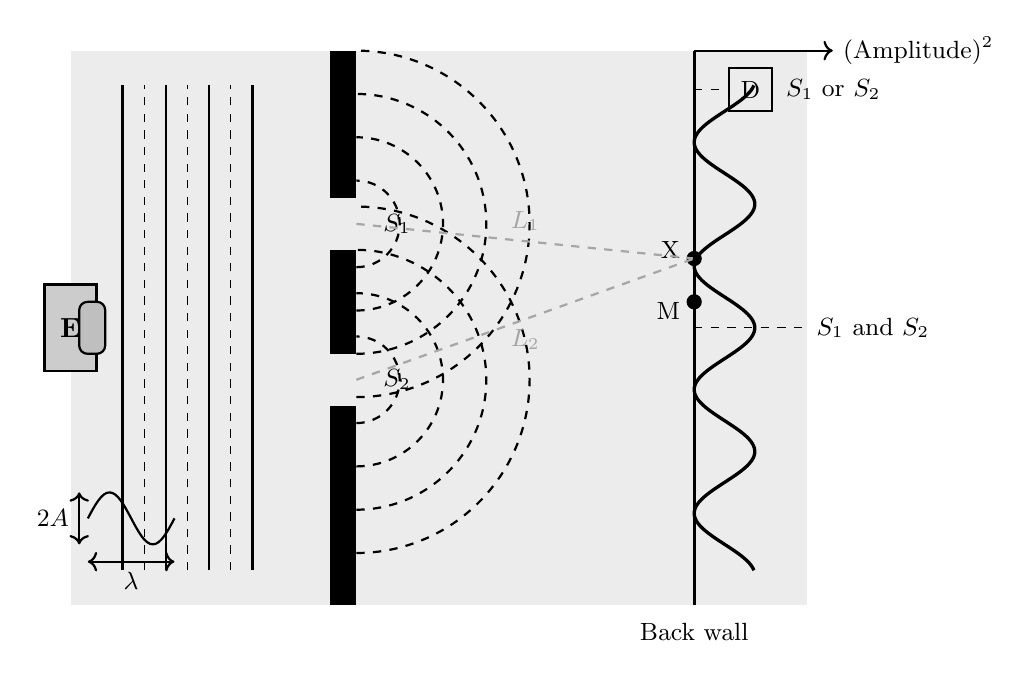
\begin{tikzpicture}[scale=1.1]

    % Background box
    \fill[gray!15] (-4,-3.2) rectangle (4.5,3.2);

    % Incoming plane waves
    \foreach \x in {-3.4, -2.9, -2.4, -1.9}{
        \draw[thick] (\x, -2.8) -- (\x, 2.8);
    }
    \foreach \x in {-3.15, -2.65, -2.15}{
        \draw[dashed] (\x, -2.8) -- (\x, 2.8);
    }

    % Source box
    \draw[fill=gray!40, thick] (-4.3, -0.5) rectangle (-3.7, 0.5);
    \node at (-4.0, 0) {\textbf{E}};
    \draw[fill=gray!50, thick, rounded corners=3pt]
        (-3.9,-0.3) rectangle (-3.6,0.3);

    % Barrier
    \fill[black] (-1.0, -3.2) rectangle (-0.7, -0.9);
    \fill[black] (-1.0, -0.3) rectangle (-0.7, 0.9);
    \fill[black] (-1.0,  1.5) rectangle (-0.7, 3.2);

    % Slit labels
    \node[right, font=\small] at (-0.5, 1.2) {$S_1$};
    \node[right, font=\small] at (-0.5, -0.6) {$S_2$};

    % Semicircles opening to the RIGHT from S1 at (-0.7, 1.2)
    \foreach \r in {0.5, 1.0, 1.5, 2.0}{
        \draw[thick, dashed]
            (-0.7, 1.2-\r) arc[start angle=-90, end angle=90, radius=\r];
    }

    % Semicircles opening to the RIGHT from S2 at (-0.7, -0.6)
    \foreach \r in {0.5, 1.0, 1.5, 2.0}{
        \draw[thick, dashed]
            (-0.7, -0.6-\r) arc[start angle=-90, end angle=90, radius=\r];
    }

    % Points X and M
    \fill (3.2, 0.8) circle (2.5pt);
    \node[left, font=\small] at (3.15, 0.9) {X};
    \fill (3.2, 0.3) circle (2.5pt);
    \node[left, font=\small] at (3.15, 0.2) {M};

    % Path lines L1 and L2
    \draw[gray!70, dashed, thick] (-0.7, 1.2) -- (3.2, 0.8)
        node[midway, above, font=\small] {$L_1$};
    \draw[gray!70, dashed, thick] (-0.7, -0.6) -- (3.2, 0.8)
        node[midway, below, font=\small] {$L_2$};

    % Back wall
    \draw[very thick] (3.2, -3.2) -- (3.2, 3.2);
    \node[below, font=\small] at (3.2, -3.3) {Back wall};

    % Interference pattern
    \draw[very thick] plot[domain=-2.8:2.8, samples=200, variable=\y]
        ({3.2 + 0.7*(cos(deg(2.2*\y)))^2}, \y);

    % Amplitude^2 axis
    \draw[->, thick] (3.2, 3.2) -- (4.8, 3.2)
        node[right, font=\small] {(Amplitude)$^2$};

    % Detector box D
    \draw[thick] (3.6, 2.5) rectangle (4.1, 3.0);
    \node[font=\small] at (3.85, 2.75) {D};

    % Reference lines
    \draw[dashed] (3.2, 2.75) -- (3.55, 2.75);
    \node[right, font=\small] at (4.15, 2.75) {$S_1$ or $S_2$};
    \draw[dashed] (3.2, 0.0) -- (4.5, 0.0)
        node[right, font=\small] {$S_1$ and $S_2$};

    % Wave annotation
    \draw[thick] (-3.8,-2.2) sin (-3.55,-1.9) cos (-3.3,-2.2)
                              sin (-3.05,-2.5) cos (-2.8,-2.2);
    \draw[<->, thick] (-3.9,-1.9) -- (-3.9,-2.5)
        node[midway, left, font=\small] {$2A$};
    \draw[<->, thick] (-3.8,-2.7) -- (-2.8,-2.7)
        node[midway, below, font=\small] {$\lambda$};

\end{tikzpicture}
\caption{The double slit experiment}
\label{fig:double_slit}
\end{figure}
\begin{figure}[H]
\centering
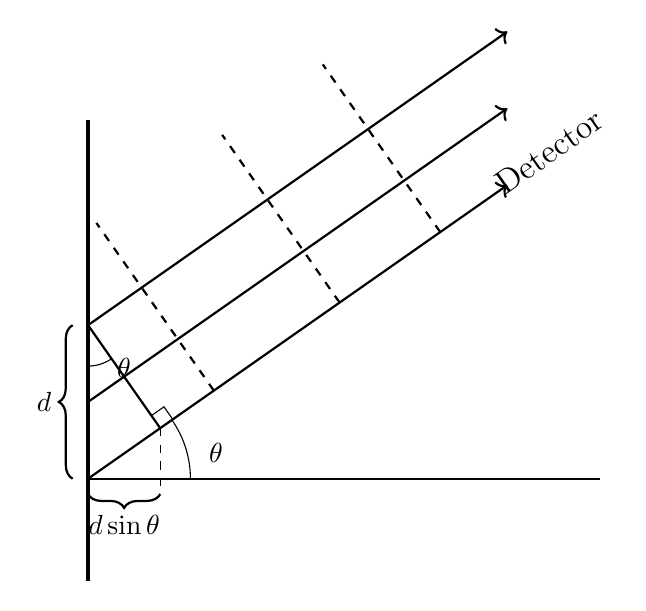
\begin{tikzpicture}[scale=1.3]

    % Barrier
    \draw[very thick] (0, -1) -- (0, 3.5);

    % d brace on the left
    \draw[thick, decorate, decoration={brace, amplitude=5pt}]
        (-0.15, 0) -- (-0.15, 1.5)
        node[midway, left, xshift=-4pt] {$d$};

    % Horizontal reference line from lower slit
    \draw[thick] (0, 0) -- (5, 0);

    % Angle theta at lower slit from horizontal
    \draw (1.0, 0) arc[start angle=0, end angle=35, radius=1.0];
    \node at (1.25, 0.25) {$\theta$};

    % Three parallel rays at 35 degrees
    \draw[->, thick] (0, 0) -- ++(35:5.0);
    \draw[->, thick] (0, 1.5) -- ++(35:5.0);
    \draw[->, thick] (0, 0.75) -- ++(35:5.0);

    % Wavefront dashes perpendicular to rays (angle 125)
    \draw[dashed, thick] ($(0,0)+(35:1.5)$) -- ++(125:2.0);
    \draw[dashed, thick] ($(0,0)+(35:3.0)$) -- ++(125:2.0);
    \draw[dashed, thick] ($(0,0)+(35:4.2)$) -- ++(125:2.0);

    % Perpendicular from upper slit to lower ray
    \coordinate (foot) at ($(0,0)!(0,1.5)!(35:6)$);

    % Line from upper slit to foot
    \draw[thick] (0, 1.5) -- (foot);

    % Right angle mark at foot
    \draw ($(foot)+(125:0.15)$) -- ++(35:0.15) -- ++(305:0.15);

    % Angle theta at upper slit
    \draw (0, 1.5) ++(270:0.4) arc[start angle=270, end angle=305, radius=0.4];
    \node at (0.35, 1.08) {$\theta$};

    % d sin theta brace at bottom
    \draw[thick, decorate, decoration={brace, amplitude=5pt, mirror}]
        (0, -0.15) -- (foot |- 0,-0.15)
        node[midway, below, yshift=-4pt] {$d\sin\theta$};

    % Vertical line from foot down for the brace reference
    \draw[dashed] (foot) -- (foot |- 0,-0.15);

    % Detector label
    \node[rotate=35, font=\large] at (4.5, 3.2) {Detector};

\end{tikzpicture}
\caption{Path difference in the double slit experiment}
\label{fig:path_diff}
\end{figure}
Clearly each ray travels different distances before it hits the screen, and the difference between these two distances will tell us if we have constructive or destructive interference.
\begin{align}
		L_2 - L_1 &= n\lambda \hspace{0.4cm}\text{(constructive interference)}\\
		L_2 - L_1 &= \left(n+\frac{1}{2}\right)\lambda\hspace{0.4cm}\text{(destructive interference)}
\end{align}
If our distance from the screen is $D\gg d$, we get
\begin{align}
	d\sin\theta &= n\lambda \hspace{0.4cm}\text{(constructive)}\\
	d\sin\theta &= \left(n + \frac{1}{2}\right)\lambda \hspace{0.4cm}\text{(destructive)}.
\end{align}
We are interested in $d\sin\theta$ because that's the extra distance the bottom wave travels, which gives us the path difference. If you want to measure things along the $y$ direction we can say
\begin{equation}
		\sin\theta \approx \frac{y}{D}
\end{equation}
From our diagram, we'd measure $y$ from the bottom slit. This implies
\begin{align}
	y &= \frac{n\lambda D}{d}\hspace{0.4cm}\text{(constructive)}\\
	y &= \frac{\left(n + \frac{1}{2}\right)\lambda D}{d}\hspace{0.4cm}\text{(destructive)}
\end{align}
Let's look at the functional form of the intensity. Let's say
\begin{align*}
	\psi_1 = Ae^{i(kr_1 - \omega t)}\\
	\psi_2 = Ae^{i(kr_2 - \omega t)}
\end{align*}
Where $r_1$, $r_2$ are what $L_1$ and $L_2$ represented previously. We want to show
\begin{equation}
		I \propto \abs{\psi}^2.
\end{equation}
To do this,
\begin{align*}
	\abs{\psi}^2 &= A^2\abs{e^{ikr_1}+e^{ikr_2}}^2\\
	&= A^2\left(e^{ikr_1}+e^{ikr_2}\right)\left(e^{-ikr_1}+e^{-ikr_2}\right)\\
	&= A^2\left(2 + e^{ik(r_1-r_2)} + e^{ik(r_2-r_1)}\right)\\
	&= 2A^2\left(1+ \cos k(r_1 - r_2)\right)
\end{align*}
Then from the power-reduction identity $1+\cos\theta = 2\cos^2\!\frac{\theta}{2}$,
\begin{equation}
		I = 4A^2\cos^2 \left[\frac{k(r_1-r_2)}{2}\right]
\end{equation}
Then clearly the cosine is maximized when $\frac{k(r_1-r_2)}{2} = n\pi$ where $n = 0,1,2\dots$. But $k = 2\pi / \lambda$ implies
\begin{align*}
	\frac{2\pi}{\lambda} \frac{r_1 - r_2}{2} &= n\pi\\
	\Rightarrow r_1-r_2 &= n\lambda
\end{align*}

\section{Lecture 6 (Post Quiz)}
\subsection{Doppler Shift} There are two cases
\begin{itemize}
	\item The source is moving
	\item The observer is moving
\end{itemize}
\subsubsection{Moving Sources}
Let's say we have a sound source emitting waves that propagate outwards like spheres. The distance between the maxima is the wavelength $\lambda$, then we know
\begin{equation}
	v=\lambda f
\end{equation}
As the source moves, it keeps emitting waves, but there are still "residual" waves from the previous position. This changes the wavelength,
\begin{equation}
	\lambda' = \lambda - u T = \lambda -\frac{u}{f}
\end{equation}
Then we can write
\begin{equation}
	f' = \frac{v}{\lambda'} = \frac{v}{\lambda -u/f} = f\frac{1}{1-u/v}
\end{equation}
Note that $v$ is the speed of the sound wave w.r.t the air.
\subsubsection{Moving Observer}
Now an observer moves towards the wave with speed $u$. The wave front is moving with speed $v$ towards the observer, so the relative speed is $v+u$. So the frequency is
\begin{equation}
	f' = \frac{u+v}{\lambda} = \frac{u+v}{v/f} = f(1+u/v)
\end{equation}
Doing a Taylor expansion of (6.3)
\begin{equation}
	f' = f\left(1+\frac{u}{v} + \left(\frac{u}{v}\right)^2 + \cdots\right)
\end{equation}
You can see that the moving observer and moving source Doppler shift agree to first order in $u/v$; they differ only at second order, so they are close when $u$ is small.
\begin{figure}[H]
\centering
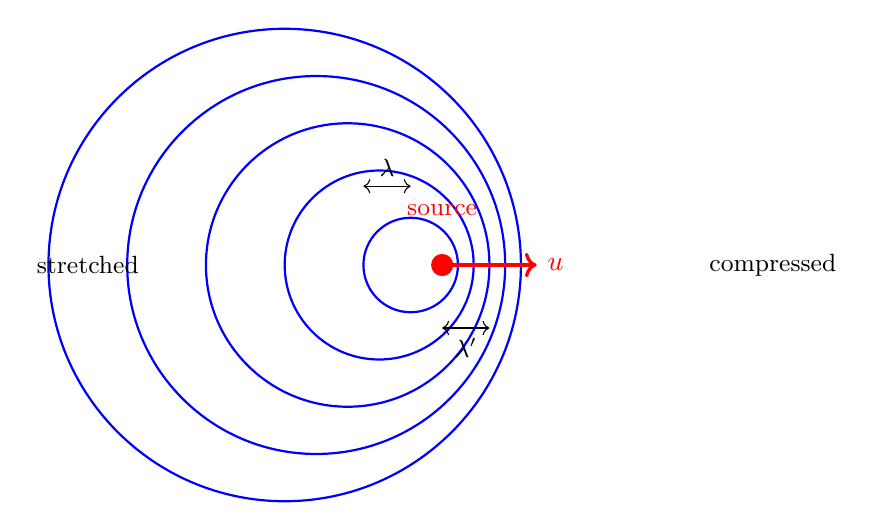
\begin{tikzpicture}[scale=1.0]

    % Circles centered at past source positions
    \foreach \i in {1, 2, 3, 4, 5}{
        \draw[blue, thick] ({-\i*0.4}, 0) circle ({\i*0.6});
    }

    % Current source position
    \fill[red] (0, 0) circle (4pt);

    % Velocity arrow
    \draw[->, very thick, red] (0, 0) -- (1.2, 0)
        node[right] {$u$};
    \node[above, red, font=\small] at (0, 0.5) {source};

    % Lambda prime
    \draw[<->] (0, -0.8) -- (0.6, -0.8)
        node[midway, below, font=\small] {$\lambda'$};

    % Lambda
    \draw[<->] (-0.4, 1.0) -- (-1.0, 1.0)
        node[midway, above, font=\small] {$\lambda$};

    % Direction labels far out
    \node[font=\small] at (4.2, 0) {compressed};
    \node[font=\small] at (-4.5, 0) {stretched};

\end{tikzpicture}
\caption{Moving source Doppler shift. Wavefronts are compressed ahead
($\lambda' < \lambda$) and stretched behind.}
\label{fig:doppler_source}
\end{figure}

\begin{figure}[H]
\centering
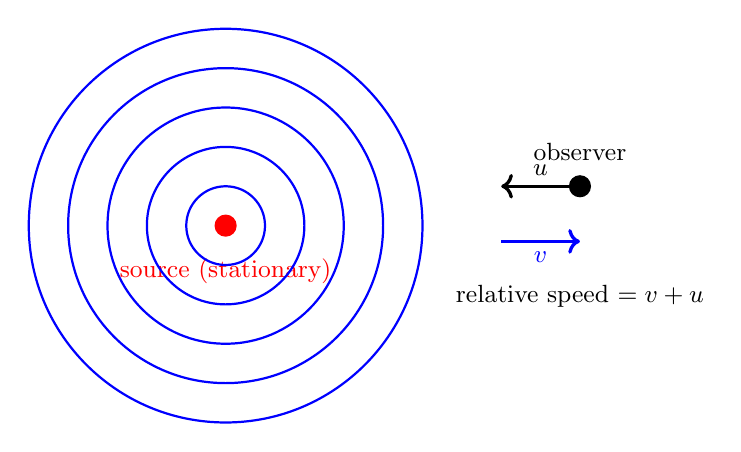
\begin{tikzpicture}[scale=1.0]

    % Stationary source
    \fill[red] (0, 0) circle (4pt);
    \node[below, red, font=\small] at (0, -0.3) {source (stationary)};

    % Concentric wavefronts
    \foreach \r in {0.5, 1.0, 1.5, 2.0, 2.5}{
        \draw[blue, thick] (0, 0) circle (\r);
    }

    % Observer to the right
    \fill[black] (4.5, 0.5) circle (4pt);
    \node[above, font=\small] at (4.5, 0.7) {observer};

    % u arrow
    \draw[->, very thick, black] (4.5, 0.5) -- (3.5, 0.5)
        node[midway, above, font=\small] {$u$};

    % v arrow
    \draw[->, very thick, blue] (3.5, -0.2) -- (4.5, -0.2)
        node[midway, below, font=\small] {$v$};

    % Relative speed label
    \node[font=\small] at (4.5, -0.9)
        {relative speed $= v + u$};

\end{tikzpicture}
\caption{Moving observer Doppler shift. The observer moves toward the
stationary source with speed $u$, increasing relative wavefront speed to $v+u$.}
\label{fig:doppler_observer}
\end{figure}
\section{Lecture 7}
\subsection{Doppler Shift (Continued)}
With wind moving at speed $w$, we can consider more interesting cases. The general result, with all speeds measured along the line from source to observer, is
\begin{equation}
	f' = f\,\frac{v + v_{\text{obs}}}{v - v_{\text{src}}}
\end{equation}
where $v_{\text{obs}}$ is the speed of the observer relative to the air (positive when moving \emph{toward} the source) and $v_{\text{src}}$ is the speed of the source relative to the air (positive when moving \emph{toward} the observer). Both numerator and denominator can be shifted by the wind speed $w$ since the wave speed $v$ is fixed relative to the air.
\subsection{Interference}
Recall that in two-slit interference with slits a distance $d$ apart, the maxima are given by
\begin{equation}
	d\sin\theta = n\lambda
\end{equation}
and the minima by
\begin{equation}
	d\sin\theta = \left(n+\frac{1}{2}\right)\lambda
\end{equation}
With one slit, of width $a$, the wave \textbf{diffracts}, and we get on the screen a single-slit diffraction pattern. It looks like a broad maximum at the middle with subsequent smaller maxima. The first minimum is found at $a\sin\theta = \lambda$.

\begin{figure}[H]
\centering
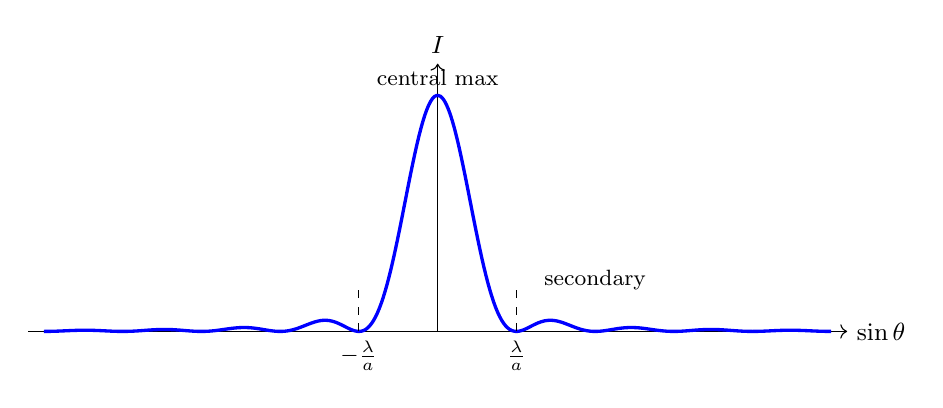
\begin{tikzpicture}[scale=1.0]
    % axes
    \draw[->] (-5.2,0) -- (5.2,0) node[right, font=\small] {$\sin\theta$};
    \draw[->] (0,0) -- (0,3.4) node[above, font=\small] {$I$};

    % single-slit intensity: I ~ (sin(x)/x)^2, with x = pi a sin(theta)/lambda.
    % Plot variable u runs over the screen; here u in [-5,5] spans several minima.
    \draw[blue, very thick, domain=-5:5, samples=400]
        plot (\x, {abs(\x)<0.001 ? 3.0 :
                   3.0*(sin(deg(\x*pi/1.0))/(\x*pi/1.0))^2});

    % mark the first minima at u = +/- 1  (a sin theta = lambda)
    \draw[dashed] (1,0) -- (1,0.55);
    \draw[dashed] (-1,0) -- (-1,0.55);
    \node[below, font=\footnotesize] at (1,0)  {$\frac{\lambda}{a}$};
    \node[below, font=\footnotesize] at (-1,0) {$-\frac{\lambda}{a}$};

    % central / secondary maxima labels
    \node[font=\footnotesize, above] at (0,3.0) {central max};
    \node[font=\footnotesize] at (2.0,0.65) {secondary};
\end{tikzpicture}
\caption{Single-slit diffraction intensity on the screen, $I \propto
\big(\sin\beta / \beta\big)^2$ with $\beta = \pi a\sin\theta/\lambda$. A broad
central maximum is flanked by much weaker secondary maxima; the first minima
occur at $a\sin\theta = \pm\lambda$.}
\label{fig:single_slit}
\end{figure}
\subsection{Beats}
Say we have two frequencies $\omega_1, \omega_2$ with $\omega_1 - \omega_2 \ll \omega_1 + \omega_2$. We will add them
\begin{equation}
	\psi = \psi_1 + \psi_2 = A\cos(\omega_1 t) + A\cos(\omega_2 t)
\end{equation}
With the cosine angle addition formulae, we get
\begin{equation}
	\psi(t) = 2A\cos\left(\frac{(\omega_1 + \omega_2)t}{2}\right)\cos\left(\frac{(\omega_1 - \omega_2)t}{2}\right)
\end{equation}
Define $\Delta\omega = \omega_1 - \omega_2$ and $\bar{\omega} = (\omega_1 + \omega_2)/2$; then $\Delta \omega \ll \bar{\omega}$. The result is a fast oscillation at $\bar\omega$ modulated by a slow envelope at $\Delta\omega/2$.
\subsection{Wave Packets}
If we now have two waves added
\begin{equation}
    \psi(x,t) = A\cos(k_1 x-\omega_1 t) + A\cos(k_2 x - \omega_2 t) = 2A\cos\left(\frac{k_1 + k_2}{2}x - \frac{\omega_1 + \omega_2}{2}t\right)\cos\left(\frac{k_1-k_2}{2}x-\frac{\omega_1 - \omega_2}{2}t\right)
\end{equation}
We want to deal with the spatial properties of this wave, so fix $t=0$.

\begin{figure}[H]
\centering
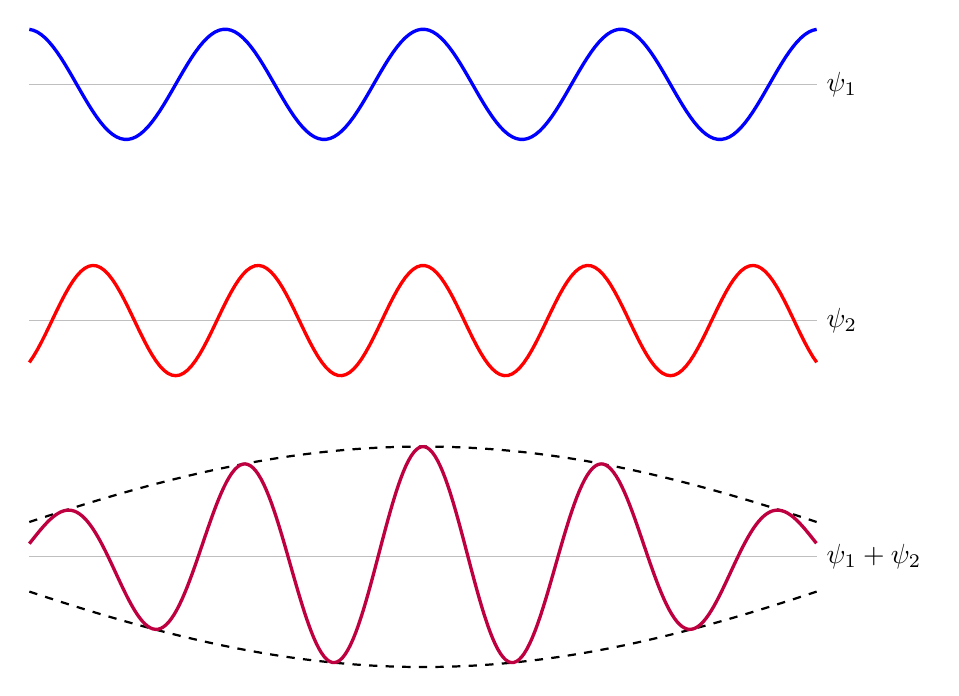
\begin{tikzpicture}[scale=1.0]

    % psi_1 (top)
    \draw[gray!50, thin] (-5, 3) -- (5, 3);
    \draw[blue, very thick, domain=-5:5, samples=200]
        plot (\x, {3 + 0.7*cos(deg(2.5*\x))});
    \node[right] at (5, 3) {$\psi_1$};

    % psi_2 (middle)
    \draw[gray!50, thin] (-5, 0) -- (5, 0);
    \draw[red, very thick, domain=-5:5, samples=200]
        plot (\x, {0 + 0.7*cos(deg(3.0*\x))});
    \node[right] at (5, 0) {$\psi_2$};

    % psi_1 + psi_2 (bottom) with envelope
    \draw[gray!50, thin] (-5, -3) -- (5, -3);
    \draw[black, dashed, thick, domain=-5:5, samples=200]
        plot (\x, {-3 + 1.4*cos(deg(0.25*\x))});
    \draw[black, dashed, thick, domain=-5:5, samples=200]
        plot (\x, {-3 - 1.4*cos(deg(0.25*\x))});
    \draw[purple, very thick, domain=-5:5, samples=300]
        plot (\x, {-3 + 0.7*cos(deg(2.5*\x)) + 0.7*cos(deg(3.0*\x))});
    \node[right] at (5, -3) {$\psi_1 + \psi_2$};

\end{tikzpicture}
\caption{Two waves $\psi_1$ (blue) and $\psi_2$ (red) and their superposition (purple) with beat envelope (dashed).}
\label{fig:two_wave_packet}
\end{figure}
As we add infinitely many waves with wave numbers between $k_1$ and $k_2$, we get the following.

\begin{figure}[H]
\centering
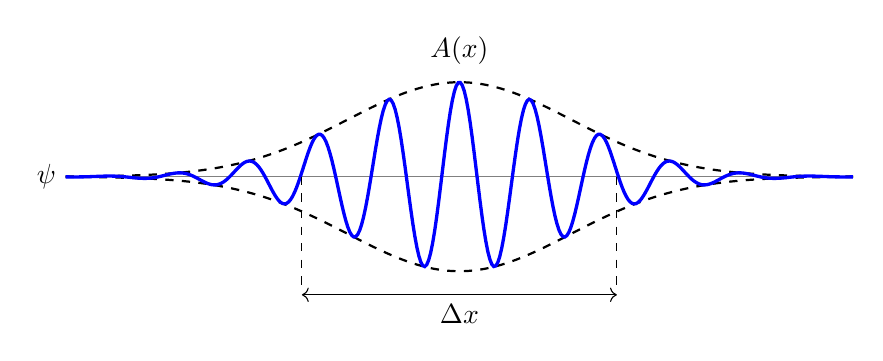
\begin{tikzpicture}[scale=1.0]
    \draw[gray, thin] (-5,0) -- (5,0);
    \node[left] at (-5, 0) {$\psi$};

    % Gaussian envelope
    \draw[dashed, thick, domain=-5:5, samples=200]
        plot (\x, {1.2*exp(-\x*\x/4)});
    \draw[dashed, thick, domain=-5:5, samples=200]
        plot (\x, {-1.2*exp(-\x*\x/4)});

    % Wave packet
    \draw[blue, very thick, domain=-5:5, samples=400]
        plot (\x, {1.2*exp(-\x*\x/4)*cos(deg(7*\x))});

    % Annotations
    \draw[<->] (-2, -1.5) -- (2, -1.5)
        node[midway, below] {$\Delta x$};
    \draw[dashed] (-2, 0) -- (-2, -1.4);
    \draw[dashed] (2, 0) -- (2, -1.4);
    \node[above] at (0, 1.3) {$A(x)$};
\end{tikzpicture}
\caption{Wave packet formed by superposition of infinitely many waves with wave numbers between $k_1$ and $k_2$, localized over a region $\Delta x$.}
\label{fig:continuous_wave_packet}
\end{figure}
\subsection{More on sound, pressure and fluids}
Let's say we have sound propagating through a pipe. We have regions of lower and higher density. These lower and higher density regions form a longitudinal wave. These alternating density regions form alternating pressures $P$. The sound speed is given by
\begin{equation}
	v_s = \sqrt{\frac{B}{\rho}}
\end{equation}
where $B$ is the bulk modulus (the measure of how "stiff" something is). The pressure is defined by
\begin{equation}
	P = \frac{F}{A}
\end{equation}
with units $\frac{N}{m^2} = $ Pa. Atmospheric pressure is
\begin{equation}
	P_{atm} = 1.013\times 10^5 \hspace{0.2cm}\text{Pa}
\end{equation}
The bulk modulus is defined as
\begin{equation}
	B = -V\frac{dP}{dV}  = -\frac{\Delta P}{\Delta V/V} = \frac{1}{\text{compressibility}}
\end{equation}
\section{Lecture 8}
\subsection{The Wave Equation for Sound Waves}
Recall
\begin{align*}
	\pdd{\psi(x,t)}{x} = \frac{1}{v^2}\pdd{\psi}{t}\\
	v = \sqrt{\frac{T}{\mu}}
\end{align*}
Now, in air
\begin{align*}
	v = \sqrt{\frac{B}{\rho}}\\
	B = -\frac{\Delta P}{\Delta V/V}
\end{align*}
If we have a column with cross sectional area $A$, and $w'$ representing its new width
\begin{align*}
	w' &= \Delta x + s(x+\Delta x,t) - s(x,t)\\
	&= \Delta x + \pd{s(x,t)}{x}\Delta x
\end{align*}
\begin{figure}[H]
\centering
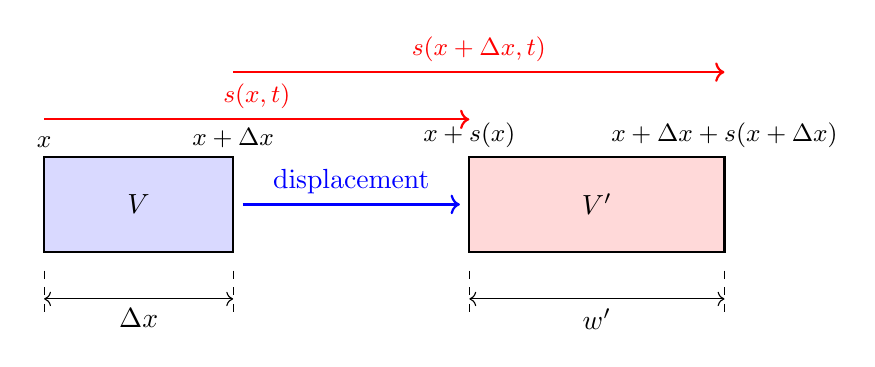
\begin{tikzpicture}[scale=1.2]

    % Original column
    \fill[blue!15] (0,-0.5) rectangle (2, 0.5);
    \draw[thick] (0,-0.5) rectangle (2, 0.5);
    \draw[dashed] (0,-0.7) -- (0,-1.2);
    \draw[dashed] (2,-0.7) -- (2,-1.2);
    \draw[<->] (0,-1.0) -- (2,-1.0) node[midway, below] {$\Delta x$};
    \node at (1, 0) {$V$};

    \node[above, font=\small] at (0, 0.5) {$x$};
    \node[above, font=\small] at (2, 0.5) {$x+\Delta x$};

    % Displaced column
    \fill[red!15] (4.5,-0.5) rectangle (7.2, 0.5);
    \draw[thick] (4.5,-0.5) rectangle (7.2, 0.5);
    \draw[dashed] (4.5,-0.7) -- (4.5,-1.2);
    \draw[dashed] (7.2,-0.7) -- (7.2,-1.2);
    \draw[<->] (4.5,-1.0) -- (7.2,-1.0) node[midway, below] {$w'$};
    \node at (5.85, 0) {$V'$};

    \node[above, font=\small] at (4.5, 0.5) {$x+s(x)$};
    \node[above, font=\small] at (7.2, 0.5) {$x+\Delta x+s(x+\Delta x)$};

    % Arrow showing displacement
    \draw[->, thick, blue] (2.1, 0) -- (4.4, 0)
        node[midway, above] {displacement};

    % s(x,t) arrow
    \draw[->, red, thick] (0, 0.9) -- (4.5, 0.9)
        node[midway, above, font=\small] {$s(x,t)$};

    % s(x+Dx,t) arrow
    \draw[->, red, thick] (2, 1.4) -- (7.2, 1.4)
        node[midway, above, font=\small] {$s(x+\Delta x, t)$};

\end{tikzpicture}
\caption{Displacement of a fluid column element of width $\Delta x$ to a new width $w'$.}
\end{figure}
Then our new volume $V'$
\begin{equation}
	V' = A\cdot\left(\Delta x + \pd{s(x,t)}{x}\Delta x\right) = V + V\pd{s(x,t)}{x}
\end{equation}
Then
\begin{equation}
	\Delta V = V' - V = V\pd{s(x,t)}{x}
\end{equation}
Now if the "total pressure" $P$ is given by
\begin{equation}
	P = P_0 + \Delta P = P_0 + p
\end{equation}
where $P_0$ is the atmospheric pressure. Then
\begin{equation}
	B = \frac{-p}{\Delta V/V} \Rightarrow p = -B\pd{s(x,t)}{x}
\end{equation}
Recall that $P = F/A$. At $x$ we have $p(x)$ pushing towards the right and then $p(x+\Delta x)$ pushing towards the left. Then the net force is
\begin{equation}
	F_{net} = A\big(p(x) - p(x+\Delta x)\big) = -A\frac{\partial p}{\partial x}\Delta x
\end{equation}
\begin{figure}[H]
\centering
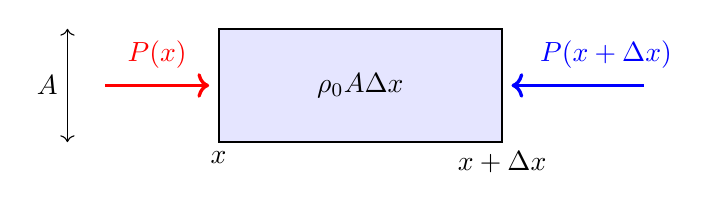
\begin{tikzpicture}[scale=1.2]

    % Column
    \fill[blue!10] (0,-0.6) rectangle (3, 0.6);
    \draw[thick] (0,-0.6) rectangle (3, 0.6);

    % Area brace on far left
    \draw[<->] (-1.6, -0.6) -- (-1.6, 0.6)
        node[midway, left] {$A$};

    % P(x) arrow
    \draw[->, very thick, red] (-1.2, 0) -- (-0.1, 0);
    \node[above, red] at (-0.65, 0.08) {$P(x)$};

    % P(x+Dx) arrow
    \draw[->, very thick, blue] (4.5, 0) -- (3.1, 0);
    \node[above, blue] at (4.1, 0.08) {$P(x+\Delta x)$};

    % Labels below
    \node[below] at (0, -0.6) {$x$};
    \node[below] at (3, -0.6) {$x + \Delta x$};

    % Mass label
    \node at (1.5, 0) {$\rho_0 A \Delta x$};

\end{tikzpicture}
\caption{Pressure forces acting on a fluid element. $P(x)$ acts rightward and
$P(x+\Delta x)$ acts leftward, giving a net force proportional to $-\pd{p}{x}$.}
\end{figure}
Where we have used a Taylor expansion. But,
\begin{align*}
	F_{net} = ma = (\rho_0 A \Delta x)\pdd{s(x,t)}{t} = -A\frac{\partial p}{\partial x}\Delta x\\
	\Rightarrow	-\pd{p}{x} = \rho_0\pdd{s}{t}
\end{align*}
From (8.4), $p = -B\pd{s}{x}$, so $\pd{p}{x} = -B\pdd{s}{x}$. Combining with $-\pd{p}{x} = \rho_0\pdd{s}{t}$ gives
\begin{equation*}
	-B\pdd{s}{x} = -\rho_0\pdd{s}{t}
\end{equation*}
Then we get the equation
\begin{equation}
	\pdd{s}{x} = \frac{1}{v^2} \pdd{s}{t},\hspace{0.4cm}v =\sqrt{\frac{B}{\rho_0}}
\end{equation}
The solution to this is of course
\begin{equation}
	s(x,t) = S_0\sin(kx-\omega t),\hspace{0.4cm} v=\frac{\omega}{k}
\end{equation}
\begin{figure}[H]
\centering
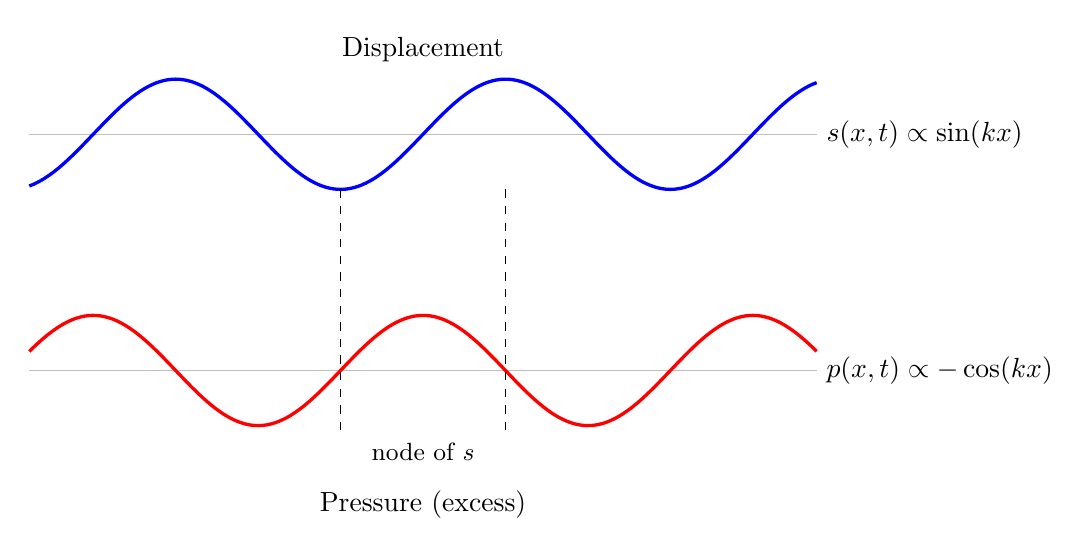
\begin{tikzpicture}[scale=1.0]

    \draw[gray!50, thin] (-5, 2) -- (5, 2);
    \draw[gray!50, thin] (-5, -1) -- (5, -1);

    % Displacement s(x,t) - sine
    \draw[blue, very thick, domain=-5:5, samples=200]
        plot (\x, {2 + 0.7*sin(deg(1.5*\x))});
    \node[right] at (5, 2) {$s(x,t) \propto \sin(kx)$};

    % Pressure p(x,t) - cosine
    \draw[red, very thick, domain=-5:5, samples=200]
        plot (\x, {-1 + 0.7*cos(deg(1.5*\x))});
    \node[right] at (5, -1) {$p(x,t) \propto -\cos(kx)$};

    % Dashed vertical lines
    \draw[dashed] (1.05, 1.3) -- (1.05, -1.8);
    \draw[dashed] (-1.05, 1.3) -- (-1.05, -1.8);

    \node[below, font=\small] at (0, -1.8) {node of $s$};

    \node[above] at (0, 2.8) {Displacement};
    \node[below] at (0, -2.4) {Pressure (excess)};

\end{tikzpicture}
\caption{Displacement $s(x,t)$ (blue) and excess pressure $p(x,t)$ (red) for a
sound wave. Pressure nodes coincide with displacement antinodes and vice versa.}
\end{figure}
We can use either a sine or cosine for the above. Then the excess pressure is
\begin{equation}
	p(x,t) = -BS_0k\cos(kx-\omega t)
\end{equation}
If we also take the derivative of $s(x,t)$, we get
\begin{equation}
	\pd{s}{t} = -\omega S_0 \cos(kx-\omega t)
\end{equation}
which implies that the particle velocity and excess pressure are in phase.
\subsection{The wave equation for pressure}
We know
\begin{align*}
	\pd{p}{x}  = -\rho_0\pdd{s}{t}\\
	\Rightarrow \pdd{p}{x} = -\rho_0\frac{\partial^3 s}{\partial x\,\partial t^2}\\
	\pdd{p}{t} = -B\frac{\partial^3 s}{\partial t^2\,\partial x}
\end{align*}
Therefore,
\begin{equation}
	\pdd{p}{x} = \frac{\rho_0}{B}\pdd{p}{t}
\end{equation}
\paragraph{The measures of stiffness}
For a steel rod, the stiffness is not measured by the bulk modulus, but rather Young's modulus.
\begin{equation}
	Y = \frac{F/A}{\Delta L/L}
\end{equation}
\section{Lecture 9}
\subsection{Density}
We need a way of finding $\rho_0$ from (8.10). The density is
\begin{equation}
	\rho_0 = \frac{m}{A\Delta x}
\end{equation}
After the displacement, the same mass $m$ now occupies the new width $w' = \Delta x\left(1 + \pd{s}{x}\right)$, so the new volume is $V' = A\Delta x\left(1+\pd{s}{x}\right)$.
So we get
\begin{equation}
	\rho = \frac{m}{A\Delta x \left(1 + \pd{s}{x}\right)}\approx \frac{m}{A\Delta x}\left(1-\pd{s}{x}\right) = \rho_0\left(1-\pd{s}{x}\right)
\end{equation}
\subsection{Young's Modulus and the Wave Equation for a Steel Rod}
Say we have a rod of steel that we want sound to propagate through.
\begin{equation}
	v = \sqrt{\frac{\text{elastic}}{\text{inertia}}}
\end{equation}
If you apply a force $F$ on both ends of the steel rod, it will compress. Say the length of the rod is $L$ and the cross-sectional area $A$. Intuitively, the pressure on the rod is proportional to how much it compresses (lengthwise):
\begin{equation}
	\frac{F}{A} = Y\frac{\Delta L}{L}
\end{equation}
Where $Y$ is the constant of proportionality, or \textbf{Young's Modulus}, which depends on the material. Also $F/A = \sigma$ is called the \textbf{stress}, and $\Delta L/L = \epsilon$ is called the \textbf{strain}.
\begin{equation}
	Y = \frac{\sigma}{\epsilon}
\end{equation}
Take an interval of the rod between $x$ and $x+\Delta x$. Let the displacements be given by $\psi(x,t),\psi(x+\Delta x,t)$. Let's assume that in this interval the rod is being expanded and not compressed. This implies that, internally, there are forces on the walls that make it want to compress.
\begin{align*}
	\frac{\Delta L}{L} &= \frac{1}{\Delta x}\left(\psi(x+\Delta x) - \psi(x)\right)= \pd{\psi}{x}\\
	\Rightarrow \frac{F}{A} &= Y\pd{\psi}{x}\\
	\Rightarrow F_{l} + F_{r} &=A Y\left(\pd{\psi}{x}\right)_{x+\Delta x} - AY \left(\pd{\psi}{x}\right)_{x}=\rho A \Delta x\,\pdd{\psi(x,t)}{t}
\end{align*}
Note the signs. There are internal forces trying to compress the material in that interval, but there is an equal and opposite force acting in the other direction acting on the mass; this gives the acceleration of that interval. Then
\begin{equation}
	\pdd{\psi}{t}=\frac{Y}{\rho}\pdd{\psi}{x}
\end{equation}
\subsection{Energy of a Sound Wave}
Recall that for a string, the energy density per unit length was given by
\begin{equation*}
	u = \mu A^2\omega^2\sin^2(kx-\omega t)
\end{equation*}
And the average energy was
\begin{equation*}
	\bar{u} = \frac{1}{2}\mu A^2\omega^2
\end{equation*}
And the power was
\begin{equation*}
	P = \frac{1}{2}\mu vA^2\omega^2.
\end{equation*}
Note that here $A$ was the amplitude, not the area. Our total energy is obviously given by the kinetic + potential energy.
\begin{equation}
	dm = \rho_0 A\, dx
\end{equation}
where $A$ here is the area and not amplitude.
\begin{align*}
	s(x,t) &= s_0\sin(kx-\omega t)\\
	\Rightarrow v_{\text{particle}}(x,t) &= \pd{s}{t} = -s_0\omega\cos(kx-\omega t)
\end{align*}
Then
\begin{equation}
	dK = \frac{1}{2}\,dm\,v_{\text{particle}}^2 = \frac{1}{2} \rho_0 A\, dx\, s_0^2\omega^2\cos^2(kx-\omega t)
\end{equation}
Since $dU = dK$ (the maximum compression coincides with maximum particle speed, exactly as in the string case),
\begin{equation}
	\frac{\overline{dE}}{dx} = \frac{\rho_0 A s_0^2\omega^2}{2}
\end{equation}
Where we've used the time average of $\cos^2$ to get the factor of a half. The intensity ($= \frac{\text{Power}}{\text{Area}}$) is
\begin{equation}
	I = \frac{1}{2}\rho_0 v\omega^2 s_0^2
\end{equation}
Recall that $p = -Bk s_0\cos(kx-\omega t)$. But $\frac{\omega}{k} = v$, so
\begin{equation}
	p = -B\frac{\omega}{v}s_0\cos(kx-\omega t) = -v^2\rho_0\frac{\omega}{v}s_0\cos(kx-\omega t)
\end{equation}
Where we used $B = v^2\rho_0$. Then
\begin{equation}
	p_{max} = \rho_0 v\omega s_0
\end{equation}
And then the intensity is given by
\begin{equation}
	I = \frac{p_{max}^2}{2\rho_0 v} = \frac{p_{rms}^2}{\rho_0 v}
\end{equation}
\section{Lecture 10}
\subsection{Intensity continued}
Obviously $p_{max} < P_{atm} \approx 10^5$ Pa. The intensity corresponding to a pressure amplitude equal to atmospheric pressure is
\begin{equation*}
	I(p_{max} = P_{atm}) \approx 1.2\times 10^{7} \;\frac{W}{m^2}
\end{equation*}
The upper limit of intensity of a sound wave (from above) gives about $194$ dB. The lower limit of human hearing is around $-24$ dB, which corresponds to a pressure amplitude on the order of a fraction of a micropascal.
\subsection{Range of Frequencies}
What is the range of frequencies sound can propagate? We hear between $20$ and $20{,}000$ Hz. The range of frequencies that can propagate in air is roughly $0.001$ Hz to $10$ MHz.
\chapter{Fluids}
\section{Lecture 11}
Recall from the previous lecture that if we have a container with liquid and a lid/tube inserted into the container, the ratio of the forces is given by the ratio of the areas
\begin{equation}
    \frac{F_1}{F_2} = \frac{a}{A}
\end{equation}
where $a$ is the area of the lid and $A$ is the area of the container.
\subsection{Archimedes' Principle}
Qualitatively,
\begin{center}
    If you have an object in a liquid, the weight of the object is going to be less than if it were outside. That is, the weight loss
    is equal to the weight of the displaced fluid.
\end{center}
The principle is quite intuitive.
\begin{equation}
    \text{net weight} = \rho_{\text{body}}gV -\rho_{\text{fluid}}gV = (\rho_b - \rho_f)Vg = (m_b - m_f)g
\end{equation}
This tells us that if $\rho_b < \rho_f$, the body will float. The volume fraction that is submerged is given by
\begin{equation}
        f = \frac{\rho_{\text{body}}}{\rho_{\text{fluid}}}
\end{equation}
\section{Lecture 12}
\subsection{Continuity}
We've so far only talked about fluid statics. We'll move on to dynamics now. Say we have a horizontal pipe that changes diameter
at some point. We ask the question of what happens to the fluid as this diameter changes. Say the fluid is moving with some velocity $v$.
Assume we have an incompressible fluid (fixed density). If we start with a wider pipe, with velocity $v_1$,
when the pipe gets narrower the fluid moves at a new speed (in that narrower tube) $v_2$ such that $v_2 > v_1$. Say the cross-sectional
area of the wider tube is $A_1$ and the narrower one $A_2$. Let's take a segment $dx_1$ of the wider section. We take
a section of equal volume in the narrower tube of length $dx_2$. Clearly, $dx_2$ is longer than $dx_1$, since it's a narrower
tube with the same volume. Since the fluid is incompressible
\begin{equation}
    A_1\,dx_1 = A_2\,dx_2
\end{equation}
But $dx_1 = v_1\,dt$ and $dx_2 = v_2\,dt$ implies
\begin{equation}
    A_1v_1 = A_2v_2 \hspace{0.4cm}\text{(continuity equation)}
\end{equation}

\begin{figure}[H]
\centering
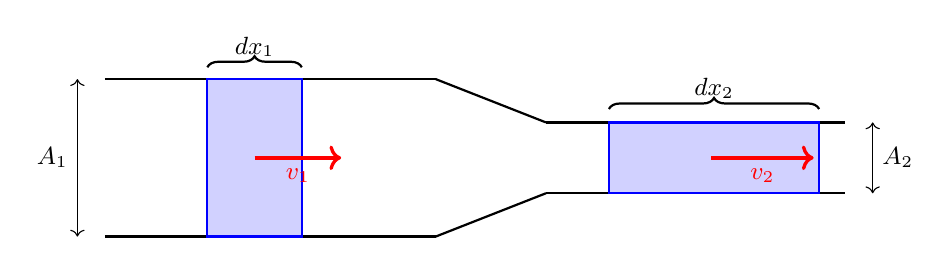
\begin{tikzpicture}[scale=1.0]

    % wide section outline
    \draw[thick] (0,1.0) -- (4.2,1.0);
    \draw[thick] (0,-1.0) -- (4.2,-1.0);
    % tapered transition
    \draw[thick] (4.2,1.0) -- (5.6,0.45);
    \draw[thick] (4.2,-1.0) -- (5.6,-0.45);
    % narrow section outline
    \draw[thick] (5.6,0.45) -- (9.4,0.45);
    \draw[thick] (5.6,-0.45) -- (9.4,-0.45);

    % shaded fluid element in wide part
    \fill[blue!18] (1.3,-1.0) rectangle (2.5,1.0);
    \draw[blue, thick] (1.3,-1.0) rectangle (2.5,1.0);
    % shaded fluid element of equal volume in narrow part
    \fill[blue!18] (6.4,-0.45) rectangle (9.07,0.45);
    \draw[blue, thick] (6.4,-0.45) rectangle (9.07,0.45);

    % cross-section area braces
    \draw[<->] (-0.35,-1.0) -- (-0.35,1.0) node[midway,left,font=\small] {$A_1$};
    \draw[<->] (9.75,-0.45) -- (9.75,0.45) node[midway,right,font=\small] {$A_2$};

    % dx braces
    \draw[decorate,decoration={brace,amplitude=4pt},thick]
        (1.3,1.15) -- (2.5,1.15) node[midway,above,font=\small] {$dx_1$};
    \draw[decorate,decoration={brace,amplitude=4pt},thick]
        (6.4,0.62) -- (9.07,0.62) node[midway,above,font=\small] {$dx_2$};

    % velocity arrows
    \draw[->,very thick,red] (1.9,0) -- (3.0,0)
        node[midway,below,font=\small] {$v_1$};
    \draw[->,very thick,red] (7.7,0) -- (9.0,0)
        node[midway,below,font=\small] {$v_2$};

\end{tikzpicture}
\caption{Flow through a constriction. The same volume of incompressible
fluid that fills the short wide element $dx_1$ must fill the longer narrow
element $dx_2$, so $A_1\,dx_1 = A_2\,dx_2$; dividing by $dt$ gives
$A_1v_1=A_2v_2$, and the fluid speeds up where the pipe narrows.}
\label{fig:continuity_pipe}
\end{figure}

We can generalize this further. If we have a compressible fluid
\begin{equation*}
    \rho_1 A_1 v_1 = \rho_2 A_2 v_2
\end{equation*}
The above is just the conservation of mass. For a more general region with volume $V$, the mass is given by
\begin{equation}
        \text{mass} = \int_V d^3r\; \rho(\mathbf{r})
\end{equation}
The change of mass is then given by
\begin{equation}
        \pd{}{t}\int_V d^3r\; \rho(\mathbf{r}) = -\oint \left(\rho(\mathbf{r})\mathbf{v}(\mathbf{r})\right)\cdot \hat{n}(\mathbf{r})\,dS .
\end{equation}
This equation is quite intuitive. The change of the mass inside comes from the component of the
velocity that is perpendicular to the surface. The negative sign comes from the fact that when the mass is flowing
out, the dot product on the RHS would be positive. We can get to the differential form quite straightforwardly using the divergence theorem
\begin{align*}
    \pd{}{t}\int_V d^3r\; \rho(\mathbf{r}) &= -\int_V d^3 r\; \nabla\cdot \left(\rho(\mathbf{r})\mathbf{v}(\mathbf{r})\right)\\
     \Rightarrow \pd{\rho(\mathbf{r})}{t} &= -\nabla \cdot \left(\rho(\mathbf{r})\mathbf{v}(\mathbf{r})\right)
\end{align*}
\begin{equation}
    \pd{\rho}{t} + \nabla\cdot(\rho \mathbf{v})=0\hspace{0.4cm}\text{(general continuity equation)}
\end{equation}
\subsection{Bernoulli's Equation}
Let's now look at a pipe that changes in height and diameter. Let's look at two segments
of the pipe as before with
\begin{align*}
    dx_1 = v_1\, dt\\
    dx_2 = v_2\, dt
\end{align*}
Let's say the energy at $(1)$ is $E_1$ and the energy at $(2)$ is $E_2$. Then,
\begin{equation}
        E_2 - E_1 = \text{net work done on the system by external forces}
\end{equation}
Since we have $E = K + U$, we get
\begin{align*}
    dK + dU = E_2 - E_1
\end{align*}
Recall that the volume of the first region is $V_1 = A_1\, dx_1 = A_1 v_1\, dt$. Then the mass
$M_1 = \rho V_1$. So we find that
\begin{align*}
    dK &= \frac{1}{2}\rho A_2 v_2\, dt\, v_2^2 - \frac{1}{2} \rho A_1 v_1\, dt\, v_1^2\\
    dU &= \rho A_2 v_2\, dt\, g h_2 - \rho A_1 v_1\, dt\, g h_1
\end{align*}
Where $h_1$ and $h_2$ are the heights of the two segments from some arbitrary reference point. The force at
(1) from the fluid on our specific segment $F_1$ is in the direction of our displacement.
\begin{align*}
    \text{work done} = F_1\, dx_1 - F_2\, dx_2 = P_1 A_1 v_1\, dt - P_2 A_2 v_2\, dt
\end{align*}
With a little algebra
\begin{align}
    \begin{split}
            P_2 + \frac{1}{2}\rho v_2^2 + \rho gh_2 = P_1 + \frac{1}{2}\rho v_1^2 +  \rho g h_1\\
            \Rightarrow P + \frac{1}{2}\rho v^2 + \rho g h = \text{const.}\hspace{0.4cm}\text{(Bernoulli Equation)}
    \end{split}
\end{align}
\paragraph{Example} Venturi meter.
\paragraph{Example} A filled container with a hole. If there is a lot of fluid, we can assume that the fluid doesn't move downwards
\textbf{in the container} very much. Let's call 1 the situation at the surface of the fluid, and 2 the situation at the hole. We also call
$h$ the height from the ground to the hole. Bernoulli's equation says
\begin{equation*}
    P_2 + \frac{1}{2}\rho v_2^2 + \rho gh_2 = P_1 + \frac{1}{2}\rho v_1^2 + \rho g h_1
\end{equation*}
Both $P_1$ and $P_2$ are atmospheric pressure, because they are open to the air. Since the hole is much smaller than the cross
section of the container, we say $v_1 \approx 0$. We are then left with the task of calculating $v_2$. If the entire height of the fluid is $H$,
\begin{align*}
    \rho g H &= \frac{1}{2}\rho v_2^2 + \rho g h \\
    \Rightarrow v_2 &= \sqrt{2g(H-h)}
\end{align*}
This is the expected result since energy conservation says $\frac{1}{2}mv_2^2 = mg(H-h)$.
\section{Lecture 13}
\subsection{Bernoulli Equation (Continued)}
Recall
\begin{equation*}
    P_1 + \frac{1}{2}\rho v_1^2 + \rho g h_1 = P_2 + \frac{1}{2}\rho v_2^2 + \rho g h_2
\end{equation*}
From the filled container with hole example from the previous lecture, we got a velocity
\begin{equation*}
    v_2 = \sqrt{2g(H-h)}
\end{equation*}
where $H$ is the height of the fluid and $h$ the height to the hole from the ground. We ask the question of how high the
hole must be from the ground such that the stream covers a horizontal distance $d$. This reduces to basic kinematics. Since $v_2$ is purely horizontal,
\begin{align*}
    h &= \frac{1}{2}gt^2\\
    d &= v_2 t\\
    \Rightarrow h &= \frac{1}{4}\frac{d^2}{H-h}
\end{align*}
\paragraph{Example} Take an airplane. Since the wing is curved, the particles that travel over the curve traverse a greater
distance than those that traverse the flat part in the same time. Thus $v_c > v_f$, and by Bernoulli's equation this implies we have a greater
pressure on the flat (bottom) side. This causes a lift force. Wings are also angled, say at an angle $\theta$ w.r.t the horizontal. Let's say this
wing is rectangular. There is still a lift force on this wing because particle collisions with the bottom side of the wing cause a change in
momentum that (by N3L) imparts an upwards force on the wing. \\

\noindent Say the wing is moving at speed $v$. The number of molecules colliding with the wing in time $dt$ is $dN$. The particles
approach the wing at an angle $\theta$ from the wing, and they are deflected at the same angle (since we have an elastic collision).
\paragraph{Example} The behavior of the air in the atmosphere. The basic idea is that the air is compressible. When we write
\begin{equation*}
    P = \rho g h
\end{equation*}
we are assuming constant $\rho$, which is not true in the atmosphere. Instead, we take a $dh$,
\begin{equation*}
    dP = -\rho(h) g\, dh
\end{equation*}
Note the negative sign because pressure decreases as height increases. In order to make progress, we need to ask the question of how $P$ depends on $\rho$. Recall the bulk modulus
\begin{equation*}
    B = -V\pd{P}{V}
\end{equation*}
Then
\begin{equation*}
    \pd{\rho}{P} = \frac{-m}{V^2}\pd{V}{P} = \frac{m}{VB} = \frac{\rho}{B}
\end{equation*}
Note that the bulk modulus depends on the density, so it would be more proper to write
\begin{equation*}
    \pd{\rho}{P} = \frac{\rho}{B(\rho)} = \frac{1}{\alpha} = \text{const.}
\end{equation*}
where the last equality holds \emph{at constant temperature}. Then
\begin{align*}
    \alpha\, d\rho &= -\rho g\, dh\\
    \Rightarrow \frac{d\rho}{\rho} &= -\frac{g}{\alpha}dh \;\Rightarrow\; \ln \rho = -\frac{g}{\alpha}h + \text{const.}
\end{align*}
Then we get
\begin{equation*}
    \rho(h) = \rho_0\, e^{-\frac{g}{\alpha}h}
\end{equation*}
Note that
\begin{equation*}
    P = \alpha \rho
\end{equation*}
is only true at constant temperature. What is $\alpha$? If we have atmospheric pressure
\begin{equation*}
    P_0 = \rho_0 g H \;\Rightarrow\; H = \frac{P_0}{\rho_0 g}
\end{equation*}
then
\begin{equation*}
    \alpha = \frac{P_0}{\rho_0} = gH
\end{equation*}
Then we are left with the isothermal-atmosphere result
\begin{equation}
    \rho(h) = \rho_0\, e^{-h/H}
\end{equation}
This is actually not as general as we can get. Note that $g = g(h)$ also depends on $h$. In fact
\begin{equation*}
    g(h) = \frac{GM}{(R+h)^2} = \frac{GM}{R^2}\frac{1}{\left(1+\frac{h}{R}\right)^2} \approx \frac{GM}{R^2}\left(1-\frac{2h}{R}\right)
\end{equation*}
\chapter{Thermodynamics}
\section{Lecture 14}
\subsection{Heat}
A few definitions to begin
\begin{itemize}
    \item \textbf{Thermal Equilibrium} -- When the body we are dealing with is of uniform temperature and is not changing after the fact.
    \item \textbf{Heat} -- Heat is a form of energy.
    \item \textbf{Walls} -- Either diathermic or adiabatic, which means it either lets heat go through or it doesn't.
    \item \textbf{Thermometers} -- Some property of the system changes with the temperature $T$. For example, if you have a rod of length
    $L$ at temperature $T_1$, then at a different temperature the length of the rod will change to some $L +\Delta L$. Experimentally
    it was found that $\Delta L = \alpha L\Delta T$, where $\Delta T = T_2 - T_1$. $\alpha$ is a property of the material called the
    \textbf{linear thermal expansion coefficient}. Sometimes $\alpha = \alpha(T)$, and this happens in practice. So we can set up another scale (such as using electrical resistance)
    and just say $T \propto \text{electrical resistance}$. We also define $\beta$, the
    \textbf{coefficient of (volume) thermal expansion}. A more formal definition would be
    \begin{equation}
        \beta = \frac{1}{V}\pd{V}{T}
    \end{equation}
\end{itemize}
\paragraph{The Zeroth Law of Thermodynamics} If $A$ is at the same temperature as $B$ and $B$ is at the same temperature as $C$,
then $A$ is at the same temperature as $C$. This implies that temperature is a well defined quantity: when we're at equilibrium there
is a well defined temperature.\\

\noindent We can now look at some results of experiment. Let's say we have a container with a gas with pressure $P$ and volume $V$. You place
a piston on top of it. You can plot $PV$ against $T$.

\begin{figure}[H]
\centering
\begin{tikzpicture}[scale=1.0]
    % axes
    \draw[->] (-0.5,0) -- (8,0) node[right] {$T$};
    \draw[->] (0,-0.4) -- (0,4.2) node[above] {$PV$};

    % the extrapolated line
    \draw[blue, very thick, domain=0:7.2, samples=2]
        plot (\x, {0.46*\x});
    \draw[blue, dashed, very thick] (0,0) -- (0,0);

    % absolute zero at origin
    \node[below left, font=\small] at (0,0) {$0$};
    \node[below, font=\small] at (0,-0.35) {(abs. zero)};

    % data points for two gases (same line)
    \fill (3.0,1.38) circle (2.2pt);
    \fill (5.6,2.576) circle (2.2pt);
    \draw[dashed] (3.0,0) -- (3.0,1.38);
    \draw[dashed] (5.6,0) -- (5.6,2.576);
    \node[below, font=\small] at (3.0,0) {$T_{\text{ice}}$};
    \node[below, font=\small] at (5.6,0) {$T_{\text{steam}}$};

    \node[blue, right, font=\small] at (6.2,3.1) {dilute gas};
\end{tikzpicture}
\caption{$PV$ versus $T$ for a dilute gas. The relation is linear, and the
line for \emph{any} dilute gas extrapolates back to the same point, which
defines absolute zero.}
\label{fig:PV_vs_T}
\end{figure}

\noindent If we define $0^{\circ}$C as the temperature where water freezes,
and $100^{\circ}$C to be the temperature at which water boils, we see that $PV$ has two different values at these temperatures. Crucially, if you replace
the gas with another, you get the same linear relationship. The only constraint on the gas is that it must be dilute.
\paragraph{Definition} The Kelvin temperature scale. Firstly, $0$ K is absolute zero. We also define
\begin{equation}
    0^{\circ}\text{C} = 273.15\;\text{K}
\end{equation}
(The triple point of water sits at $273.16$ K, very slightly above the ice point.)
We can now write the \textbf{ideal gas law} (which only works for dilute gases)
\begin{equation}
    PV = nRT \hspace{0.4cm}\text{(Ideal Gas Law)}
\end{equation}
Where $n$ is the number of \textbf{moles} in the gas.
\paragraph{Mercury Thermometer} A bulb and a thin tube are connected, with mercury filled up to a certain level (the empty space being a vacuum). The tube
is very thin.
\subsection{Specific Heat}
We denote the specific heat by $c$.
\begin{equation}
    \Delta Q = mc \,\Delta T
\end{equation}
Here, $\Delta Q$ means the amount of heat we are putting in the body. For water we have
\begin{equation*}
    c = \frac{1 \text{ cal}}{\text{gram}\cdot{}^{\circ}\text{C} }
\end{equation*}
Note that for the above it doesn't matter if we use the Celsius or Kelvin scale, since only a temperature \emph{difference} appears. Also it's useful to define
\begin{equation}
    1\text{ cal} = 4.184 \text{ J}
\end{equation}
This is not completely rigorous, since we could have $c = c(T)$.
\paragraph{Example} Say you have a body with $m_1,c_1,T_1$ and another with $m_2,c_2,T_2$ connected by a diathermic wall. You want to find
the final equilibrium temperature. This is straightforward with conservation of energy.
\subsection{Phase transformations} Let's say you have some ice and you're adding heat to it. We plot temperature as a function of heat added.

\begin{figure}[H]
\centering
\begin{tikzpicture}[scale=1.0]
    % axes
    \draw[->] (0,0) -- (10,0) node[right] {heat added $Q$};
    \draw[->] (0,-0.4) -- (0,4.2) node[above] {$T$};

    % ice warming
    \draw[blue, very thick] (0,0.6) -- (1.6,1.5);
    % melting plateau (latent heat of fusion)
    \draw[blue, very thick] (1.6,1.5) -- (4.0,1.5);
    % water warming
    \draw[blue, very thick] (4.0,1.5) -- (5.6,3.0);
    % boiling plateau (latent heat of vaporization)
    \draw[blue, very thick] (5.6,3.0) -- (9.0,3.0);
    % vapour warming
    \draw[blue, very thick] (9.0,3.0) -- (9.8,3.7);

    % temperature labels
    \draw[dashed] (0,1.5) -- (1.6,1.5);
    \node[left, font=\small] at (0,1.5) {$0^\circ$C};
    \draw[dashed] (0,3.0) -- (5.6,3.0);
    \node[left, font=\small] at (0,3.0) {$100^\circ$C};

    % phase labels
    \node[font=\footnotesize, rotate=30] at (0.8,1.4) {ice};
    \node[font=\footnotesize] at (2.8,1.2) {melting};
    \node[font=\footnotesize, rotate=43] at (4.8,2.5) {water};
    \node[font=\footnotesize] at (7.3,2.7) {boiling};
    \node[font=\footnotesize, rotate=40] at (9.4,3.5) {vapour};
\end{tikzpicture}
\caption{Temperature versus heat added for water. The flat plateaus are the
latent heats of fusion and vaporization: heat is absorbed with no change in
temperature while the phase transition takes place.}
\label{fig:phase_transitions}
\end{figure}

\noindent As you add heat it gets warmer, but then at some point you are adding heat but there is no change in temperature. That is the regime of \textbf{latent heat}.
After the ice has been converted to water, the water starts increasing its temperature (according to its specific heat), and again at some point the graph becomes flat
because of latent heat. Then when it has been converted to a gas, the temperature increases with heat again. We denote the latent heat of fusion by $L$. For water we have
\begin{align*}
    L_f &= \frac{80\text{ kcal}}{\text{kg}}\\
    L_v &= \frac{540\text{ kcal}}{\text{kg}}
\end{align*}
\section{Lecture 15}
\subsection{Viscosity}
Say you had a fluid between two plates. The top plate moves, while the bottom remains still. The
fluid "sticks" to both plates, so the fluid at the top moves at the speed of the plate, while the fluid at the bottom doesn't move. This creates
a gradient of velocity. This causes internal friction, which dissipates energy. So we'd have to correct Bernoulli's equation for these losses. Here are the assumptions that we make
to use Bernoulli's equation
\begin{itemize}
    \item Inviscid fluid (no viscosity)
    \item Incompressible
\end{itemize}
\subsection{Phase transitions}
\section{Lecture 16}
\subsection{The transfer of heat}
There are three ways heat can be transferred:
\begin{enumerate}
    \item Radiation
    \item Convection
    \item Conduction
\end{enumerate}
Radiation does not require a medium, while the other two do. The difference between convection and conduction is that in
convection the molecules actually travel. When you have a region of hot air and a region of cold air, the cold air will move down and the
hot air will move up. So in convection the medium moves. In conduction, the medium does not move. The molecules vibrate but stay in place. \\

\noindent\textbf{Thermal conductivity}, denoted by $\kappa$, is given by
\begin{equation}
    \frac{dQ}{dt} = \frac{-\kappa A}{L}(T_1- T_2)
\end{equation}
Some examples may provide some intuition
\begin{itemize}
    \item  $\kappa_{\text{water}} = 0.6$ W/mK,
    \item $\kappa_{\text{copper}} =  400$ W/mK,
    \item $\kappa_{\text{glass}} = 0.8$ W/mK.
\end{itemize}
Finding the final temperature is just a process of solving a simple differential equation. Let $Q$ be the amount of heat that has flowed from body 1 (hot) into body 2 (cold). Then body 1 loses heat and body 2 gains it:
\begin{align*}
    m_1c_1\, dT_1 &= - dQ, \qquad m_2c_2\, dT_2 = + dQ \qquad (T_1>T_2)\\
    \implies \frac{dT_1}{dt} &= -\frac{1}{m_1c_1}\frac{dQ}{dt}, \qquad \frac{dT_2}{dt} = +\frac{1}{m_2c_2}\frac{dQ}{dt}\\
    \implies \frac{d}{dt} (T_1-T_2) &= -\left(\frac{1}{m_1c_1}+ \frac{1}{m_2c_2}\right)\frac{dQ}{dt}\\
    \implies \frac{d}{dt} \Delta T &= -\left(\frac{1}{m_1c_1} + \frac{1}{m_2c_2}\right)\frac{\kappa A}{L}\Delta T\\
    \implies \frac{d}{dt}\Delta T &= -\alpha\, \Delta T,\qquad \alpha = \left(\frac{1}{m_1c_1} + \frac{1}{m_2c_2}\right)\frac{\kappa A}{L}\\
    \implies \Delta T(t) &= \big(T_1(0) - T_2(0)\big)\,e^{-t/\tau},\qquad \tau = \frac{1}{\alpha}
\end{align*}
where we used $\frac{dQ}{dt} = \frac{\kappa A}{L}\Delta T$ (heat flows from hot to cold). So $\Delta T \to 0$ as $t\to\infty$: the bodies do approach a common temperature, but only asymptotically -- equilibrium is never reached in finite time.
\subsection{Mercury Thermometer}
Recall the coefficient of thermal expansion is given by
\begin{equation*}
    \beta = \frac{1}{V}\frac{dV}{dT}
\end{equation*}
For mercury, $\beta = 0.00018\;/{}^{\circ}$C. How much does the height of the mercury change for a 1 degree change? Note that $\Delta V = \beta V \Delta T$. The mercury is incompressible, so we have to look at the
extra length/height it gains up the column. Then
\begin{align*}
    \Delta V &= \beta V \Delta T = A\,\Delta L\\
    \implies \Delta L &= \beta\frac{V\Delta T}{A}
\end{align*}
\subsection{Ideal gases}
Recall, at fixed temperature,
\begin{equation}
    PV = \text{const.}
\end{equation}
All of the graphs of $PV$ against $T$ extrapolate to the same zero, which is $0$ K. The \textbf{ideal gas law} is
\begin{equation}
    PV = Nk_BT
\end{equation}
where $N$ is the number of molecules (not atoms) and $k_B$ is the Boltzmann constant ($\approx 1.38\times 10^{-23}$ J/K).
\section{Lecture 17}
Recall
\begin{equation*}
    PV = Nk_BT
\end{equation*}
where $k_B \approx 1.38\times10^{-23}\;\frac{\text{J}}{\text{K}}$. Say we have a box with moving molecules. When one hits the wall, we assume a completely elastic collision and we get a change in momentum
\begin{equation*}
    \Delta p = 2mv
\end{equation*}
We want the total force on the box. Let's look at an area $A$ of the wall. How many molecules hit the wall
in unit time? A small volume is given by
\begin{equation*}
    dV = A v\, dt
\end{equation*}
The number of molecules that hit the wall in $dt$ is given by the density $\frac{N}{V}$ multiplied by the volume $A v\, dt$, then by $\frac{1}{2}$ (half the molecules move towards the wall, half move away) and by $\frac{1}{3}$ (on average a third of the molecules are associated with each of the three axes). So we get
\begin{equation*}
    F\, dt = \frac{N}{V}\cdot A v\, dt \cdot \frac{1}{3}\cdot\frac{1}{2}\cdot 2mv
\end{equation*}
Here $v^2$ should be understood as the mean square speed $\overline{v^2}$. Now we get the pressure trivially
\begin{equation}
    P = \frac{Nm\overline{v^2}}{3V}
\end{equation}
We assume this is a dilute gas, and that each molecule does not take up much volume relative to the box. Comparing to the ideal gas law, we see that
\begin{equation}
    \frac{1}{2}m\overline{v^2} = \bar{K} = \frac{3}{2}k_BT
\end{equation}
This tells us the important result that the average kinetic energy of a particle is a reflection of its absolute temperature. Also, the kinetic energy doesn't depend on the heaviness of the gas, if we maintain the same temperature.
\\
\noindent There are also three directions of motion, meaning there are three degrees of freedom. This means the energy per degree of freedom is
\begin{equation}
    \frac{1}{2}k_BT = \text{energy per degree of freedom}
\end{equation}
This is known as the equipartition theorem.
\section{Lecture 18}
\subsection{Kinetic Theory}
Take the box example again. Here is a different derivation.\\

\noindent If the box is of length $L$, then a particle takes time
\begin{equation}
    \Delta t = \frac{2L}{v_x}
\end{equation}
to traverse the $x$ direction of the box back and forth. With $\Delta p = 2mv_x$, the pressure for one molecule is given by
\begin{equation}
    P_1 = \frac{F_1}{A} = \frac{mv_x^2}{V}
\end{equation}
Then for all molecules,
\begin{equation}
    P = \sum_i P_i = \frac{m}{V}\sum_i v_{x,i}^2 = \frac{mN}{V}\cdot\frac{1}{N}\sum_i v_{x,i}^2 = \frac{mN}{V}\,\overline{v_x^2}
\end{equation}
By the ideal gas law, $PV = Nk_BT$, so
\begin{equation}
    \frac{1}{2}m\,\overline{v_x^2} = \frac{1}{2}k_BT
\end{equation}
Since the mean square speed splits equally among the three directions, $\overline{v^2} = 3\,\overline{v_x^2}$, and
\begin{equation}
    \frac{1}{2}m\,\overline{v^2} = \frac{3}{2}k_BT
\end{equation}
Also,
\begin{equation}
    v_{\text{rms}} = \sqrt{\overline{v^2}}
\end{equation}
\subsection{The Maxwell-Boltzmann Distribution}
This is given by
\begin{equation}
    g(v) = Cv^2e^{-\frac{1}{2}mv^2/k_BT}
\end{equation}

\begin{figure}[H]
\centering
\begin{tikzpicture}[scale=1.0]
    \draw[->] (0,0) -- (9.2,0) node[right] {$v$};
    \draw[->] (0,0) -- (0,3.8) node[above] {$g(v)$};

    % distribution: g(v) ~ v^2 exp(-m v^2 / 2kT); peak (most probable speed)
    % is at the v0 dashed line below.
    \draw[blue, very thick, domain=0:8.6, samples=300]
        plot (\x, {3.6*(\x*\x)*exp(-0.16*\x*\x)/2.3});

    % The three characteristic speeds, in their true order v0 < vbar < vrms.
    % v0 = sqrt(2kT/m), vbar = sqrt(8/pi kT/m), vrms = sqrt(3kT/m);
    % numerically the ratios are 1 : 1.128 : 1.225. Plotted at 2.5, 2.82, 3.06.
    % Curve height on g at those points (for the dashed-line tops):
    \draw[dashed] (2.50,0) -- (2.50,2.272);   % v0  - at the peak
    \draw[dashed] (2.82,0) -- (2.82,2.206);   % vbar
    \draw[dashed] (3.06,0) -- (3.06,2.098);   % vrms

    % ticks on the axis
    \foreach \xx in {2.50,2.82,3.06}{\draw (\xx,0.06) -- (\xx,-0.06);}

    % labels on a single row below, each joined to its tick by a short leader
    \node[font=\footnotesize] (lv0)  at (1.55,-0.62) {$v_0$};
    \node[font=\footnotesize] (lvb)  at (2.82,-0.95) {$\bar v$};
    \node[font=\footnotesize] (lvr)  at (4.30,-0.62) {$v_{\text{rms}}$};
    \draw[gray] (lv0) -- (2.50,-0.10);
    \draw[gray] (lvb) -- (2.82,-0.10);
    \draw[gray] (lvr) -- (3.06,-0.10);

    % annotate the peak
    \node[blue, font=\footnotesize] at (1.35,2.55) {peak of $g$};
    \draw[blue] (1.35,2.42) -- (2.42,2.30);
\end{tikzpicture}
\caption{The Maxwell-Boltzmann speed distribution $g(v)$. It rises as $v^2$
near the origin and is cut off by the Gaussian factor at large $v$, giving a
right-skewed peak. The three characteristic speeds occur in the order
$v_0 < \bar v < v_{\text{rms}}$: the most probable speed $v_0$ sits exactly at
the maximum of $g$, while the mean $\bar v$ and the root-mean-square speed
$v_{\text{rms}}$ are pulled to higher values by the long high-speed tail.}
\label{fig:maxwell_boltzmann}
\end{figure}

We normalize it so that
\begin{equation}
    \int_0^{\infty}dv\;g(v) =1
\end{equation}
\paragraph{The derivation} The molecule will have $\mathbf{v}=(v_x,v_y,v_z)$. The distribution depends on these velocities. Maxwell claimed that the distribution could be factored into functions of $v_x$, $v_y$ and $v_z$. He also claimed it would be a function of only the magnitude of the velocity. So
\begin{equation}
    F(v_x,v_y,v_z) = f(v_x)f(v_y)f(v_z) = \bar{f}\left(v_x^2 + v_y^2 + v_z^2\right)
\end{equation}
Maxwell proved mathematically that the only possible functions that satisfy the above relation are those of the form
\begin{equation}
    f(v_x) = Ce^{-\lambda v_x^2}
\end{equation}
Then you can see that, plugging it into (18.9)
\begin{equation}
    F(v_x,v_y,v_z) = C^3 e^{-\lambda (v_x^2 + v_y^2 + v_z^2)}
\end{equation}
which satisfies the fact that the distribution depends only on the magnitude of the velocity. Clearly $\lambda$ must have units of $t^2/\ell^2$. Also it must be positive (with the minus sign shown explicitly), so that the distribution doesn't diverge at infinity. Now we normalize
\begin{equation*}
    \int^{\infty}_{-\infty}dv_x\,f(v_x) = 1 = \int^{\infty}_{-\infty} dv_x\, Ce^{-\lambda v_x^2}
\end{equation*}
Here's how you do a Gaussian integral.
\begin{align*}
    &I = \int^{\infty}_{-\infty}dx\; e^{-\lambda x^2}\\
    &\implies I^2 = \int\int dx\, dy\; e^{-\lambda (x^2 + y^2)}\\
    &= 2\pi \int^{\infty}_0 dr\; r\, e^{-\lambda r^2} = \frac{\pi}{\lambda}
\end{align*}
Then it's clear that
\begin{equation}
    \int^{\infty}_{-\infty} dx\; e^{-\lambda x^2} = \sqrt{\frac{\pi}{\lambda}}
\end{equation}
So, we find that
\begin{equation}
    \int^{\infty}_{-\infty} dv_x\; Ce^{-\lambda v_x^2} = C\sqrt{\frac{\pi}{\lambda}}
\end{equation}
which fixes $C = \sqrt{\lambda/\pi}$. Also, the average of the square of $v_x$ is given, by the definition of the average, by
\begin{equation}
    \overline{v_x^2} = \int^{\infty}_{-\infty}dv_x\;v_x^2\, f(v_x) = C\int^{\infty}_{-\infty}dv_x\; v_x^2\, e^{-\lambda v_x^2}
\end{equation}
We can use Feynman's trick (differentiation under the integral sign) to compute an integral that looks like (18.14). Since $I(\lambda) = \sqrt{\pi/\lambda}$,
\begin{equation}
    \pd{I(\lambda)}{\lambda} = -\int^{\infty}_{-\infty} dx\; x^2 e^{-\lambda x^2} = -\frac{1}{2}\sqrt{\frac{\pi}{\lambda^3}}
\end{equation}
so that $\int_{-\infty}^{\infty} dx\,x^2 e^{-\lambda x^2} = \frac{1}{2}\sqrt{\pi/\lambda^3}$.
Using this result, and using $C = \sqrt{\lambda/\pi}$,
\begin{equation}
    \overline{v_x^2} = C\cdot\frac{1}{2} \sqrt{\frac{\pi}{\lambda^3}} = \frac{1}{2} \sqrt{\frac{\pi}{\lambda^3}\cdot\frac{\lambda}{\pi}}  = \frac{1}{2\lambda}
\end{equation}
Since we know $\overline{v_x^2} =\frac{k_BT}{m}$,
\begin{equation}
    \frac{1}{2\lambda} = \frac{k_BT}{m} \;\Rightarrow\; \lambda = \frac{m}{2k_BT}
\end{equation}
Therefore, we arrive at
\begin{equation}
    f(v_x) = \sqrt{\frac{m}{2\pi k_B T}}\;e^{-\frac{1}{2}mv_x^2/k_BT}
\end{equation}
Now using $F(v_x,v_y,v_z) = f(v_x)f(v_y)f(v_z)$,
\begin{equation*}
    F = \left(\frac{m}{2\pi k_B T}\right)^{3/2}e^{-\frac{1}{2}mv^2/k_BT}
\end{equation*}
Now we need to get to the probability of speed. Take a sphere, with radius $v = \sqrt{v_x^2 + v_y^2 + v_z^2}$. At any point on the boundary of the sphere, $v$ is the same, but $v_x,v_y,v_z$ vary. Take two spheres,
one with radius $v$, and the other with radius $v+dv$. You can then integrate over the shell
\begin{align*}
    \underset{\text{shell}}{\int\int\int}F(v_x,v_y,v_z)\, d^3v = 4\pi v^2\, dv\left(\frac{m}{2\pi k_BT}\right)^{3/2}e^{-\frac{1}{2}mv^2/k_BT} = g(v)\,dv
\end{align*}
We are left with the relation
\begin{equation}
    g(v) = 4\pi \left(\frac{m}{2\pi k_BT}\right)^{3/2}v^2\, e^{-\frac{1}{2}mv^2/k_BT}
\end{equation}
One checks normalization,
\begin{equation}
    \int^{\infty}_{0} dv\; g(v) = 1,
\end{equation}
and that $\overline{v^2} = \frac{3k_BT}{m}$:
\begin{equation*}
    \overline{v^2} = 4\pi\left(\frac{m}{2\pi k_BT}\right)^{3/2}\int^{\infty}_{0}dv\; v^4\, e^{-\frac{1}{2}mv^2/k_BT}
\end{equation*}
To compute this, note
\begin{equation*}
    I_4 = \int^{\infty}_{-\infty}dx\; x^4 e^{-\lambda x^2} = \frac{3}{8}\sqrt{\frac{\pi}{\lambda^5}}
\end{equation*}
Plugging this in gives the correct result. Now what about the average of $v$?
\begin{equation}
    \bar{v} = \int^{\infty}_{0}dv \cdot v \cdot g(v) = 4\pi\left(\frac{m}{2\pi k_BT}\right)^{3/2}\int^{\infty}_{0}dv\cdot v^3\, e^{-\frac{1}{2}mv^2/k_BT}
\end{equation}
Note that the integral
\begin{equation}
    I_3 = \int^{\infty}_{0} dx\cdot x^3\, e^{-\lambda x^2} = \frac{1}{2\lambda^2}
\end{equation}
Then we can plug this result in, with $\lambda = m/2k_BT$,
\begin{align*}
    \bar{v} = 4\pi\left(\frac{m}{2\pi k_BT}\right)^{3/2}\cdot\frac{1}{2}\left(\frac{2k_BT}{m}\right)^{2} = \sqrt{\frac{8}{\pi}\frac{k_BT}{m}}
\end{align*}
To find the most probable speed, look at where $g$ is maximized:
\begin{equation}
    \frac{dg}{dv} = 0 \;\Longrightarrow\; 2v_0\,e^{-\frac{m}{2}\frac{v_0^2}{k_BT}}-v_0^2\cdot\frac{m}{k_BT}\,v_0\,e^{-\frac{m}{2}\frac{v_0^2}{k_BT}} = 0
\end{equation}
Now we get the last of the three results we have been working on
\begin{align}
    v_0 &= \sqrt{\frac{2k_BT}{m}}\quad \text{(most probable)}\\
    \bar{v} &= \sqrt{\frac{8}{\pi}\frac{k_BT}{m}}\quad \text{(average)}\\
    v_{\text{rms}} &= \sqrt{\frac{3k_BT}{m}}\quad \text{(root-mean-square)}
\end{align}
\section{Lecture 19}
There were a few mistakes from the previous lecture (corrected in my notes, but the discussion of the integral is useful so I'll include it here). Here is a corrected derivation. Recall 
\begin{equation*}
    g(v) = 4\pi v^2\left(\frac{m}{2\pi kT}\right)^{3/2}e^{-\frac{1}{2}mv^2/kT}
\end{equation*}
Now when we want to compute the average speed, we have a factor of $v^3$ in the integrand. We need to solve this integral
\begin{equation*}
    \int_0^{\infty}x^3 e^{-\lambda x}
\end{equation*}
We already know 
\begin{equation*}
    I_1(\lambda) = \int^{\infty}_0 dx xe^{-\lambda x^2} = \frac{1}{2\lambda}
\end{equation*}
So, taking the deriative of $I_1$ w.r.t $\lambda$, 
\begin{equation*}
    \pd{I_1}{\lambda} = -\int^{\infty}_0 dx x^3 e^{-\lambda x} = -\frac{1}{2\lambda^2}
\end{equation*}
This means
\begin{equation}
    \bar{v} = 4\pi\left(\frac{m}{2\pi kT}\right)^{3/2}\int^{\infty}_0 dv v^3 e^{-\frac{1}{2}mv^2/kT} = 4\pi\left(\frac{m}{2\pi kT}\right)^{3/2}\cdot\frac{1}{2}\cdot \frac{(kT)^2}{\frac{1}{4}m^2} = \sqrt{\frac{8kT}{\pi m}}
\end{equation}
\subsection{The First Law of Thermodynamics}
The first law talks about the conservation of energy. The new concept we need to internalize (pun intended) is internal energy $U$. That is energy in the system 
at a given state. For a monatomic ideal gas, $U$ is the kinetic energy of the molecules. So here, that means $U = \frac{3}{2}nRT$. This is because in a monatomic ideal gas we have only three degrees of freedom, which is the motion in each 
direction. If we have more degrees of freedom, like a diatomic gas, the internal energy is going to be something different, since we have rotations too. This adds two extra degrees of freedom, so $U = \frac{5}{2}nRT$. For an ideal gas,
\begin{equation}
    U = U(T) \qquad \text{(ideal gas)}
\end{equation}
For a nonideal gas, 
\begin{equation}
    U = U(T,V) \qquad \text{(nonideal gas)}
\end{equation}
We usually draw $P$-$V$ diagrams to represnet theromdynamic situations. If $dU$ represents the change in internal energy, the first law of thermodynamics says  
\begin{equation}
    dU = \delta Q - \delta W
\end{equation}
Where $\delta Q$ is the heat \textbf{absorbed} by the system and $\delta W$ is the work done \textbf{by} the system. This means if heat is released, $\delta Q <0$ and if work is done on the system $\delta W<0$. Now, let's look more closely at work.
\begin{equation}
    \delta W = F\cdot dx = PAdx = PdV
\end{equation}
So, for ideal gasses we can write 
\begin{equation}
    dU = \delta Q - PdV \qquad \text{(first law for an ideal gas)}
\end{equation}
\section{Lecture 20}
Recall
\begin{equation*}
    v_{\text{rms}} = \sqrt{\frac{3k_BT}{m}}
\end{equation*}
Note that also,
\begin{equation}
    m = \frac{M}{N_A}
\end{equation}
where $M$ is the molar mass, and $N_A$ is Avogadro's constant. So we can write
\begin{equation}
    v_{\text{rms}} = \sqrt{\frac{3RT}{M}}
\end{equation}
where
\begin{equation}
    R = N_A\cdot k_B = 8.31\;\frac{\text{J}}{\text{K}\cdot\text{mol}}
\end{equation}
\subsection{Mean free path}
The mean free path is how far a molecule goes before it collides with another molecule. This intuitively depends on the density of the molecules and their diameter (because when the particles collide their centers are a distance $d$ apart, where $d$ is the molecular diameter).
\begin{equation}
    l = \frac{\text{path length}}{\text{no. of collisions}} = \frac{vt}{\frac{N}{V}\cdot vt\cdot\pi d^2}
\end{equation}
The denominator is the density multiplied by the volume of the collision cylinder (with radius $d$, the molecular diameter, since the line connecting two colliding centers has length $d$). However, we need one more correction. We are assuming every other molecule is staying still; accounting for their motion adds a factor of $\sqrt{2}$ in the denominator.
We call $\sigma = \pi d^2$ and $\frac{N}{V} = n_0$. Plugging these definitions into (20.4) and simplifying
\begin{equation}
    l = \frac{1}{\sqrt{2}\,n_0\sigma}
\end{equation}
Using the ideal gas law, $\frac{N}{V} = n_0 = \frac{P}{k_BT}$. So we can write
\begin{equation}
    l = \frac{k_BT}{\sqrt{2}\,P\pi d^2}
\end{equation}
Now we turn to the intermolecular distance $d_i$. This is roughly given by
\begin{equation}
    d_i =\left(\frac{V}{N}\right)^{1/3} = \left(\frac{k_BT}{P}\right)^{1/3} \approx 3.3\text{ nm}
\end{equation}
We can then ask what the time between collisions is
\begin{equation}
    \tau = \frac{l}{\bar v}
\end{equation}
For sound, recall, at constant temperature,
\begin{align*}
    v_{\text{sound}} &= \sqrt{\frac{B}{\rho}}\quad \text{ where } B = -V\pd{P}{V} = -V\cdot\left(-\frac{Nk_BT}{V^2}\right) = \frac{Nk_BT}{V} = P\\
    \implies v_{\text{sound}} &= \sqrt{\frac{P}{\rho}} = \sqrt{\frac{Nk_BT}{V}\cdot\frac{V}{mN}} = \sqrt{\frac{k_BT}{m}} = \sqrt{\frac{N_Ak_BT}{N_Am}} = \sqrt{\frac{RT}{M}}
\end{align*}
For air, this gives something like $290$ m/s. This is not great because we assumed the temperature was constant -- this is the \emph{isothermal} (Newton) speed of sound, and it comes out about $18\%$ too low. If the temperature were not held constant the term $\pd{P}{V}$ would change: the correct \emph{adiabatic} treatment gives $v = \sqrt{\gamma P/\rho}$. Now what happens when we have mixtures of gases? Everything just adds up. We have what are called partial pressures, where the total pressure is given by
\begin{equation}
    P = (N_1 + N_2)\frac{k_BT}{V} = P_1 + P_2 \qquad \text{(Dalton's Law)}
\end{equation}
\subsection{The first law revisited}
Recall
\begin{equation*}
    \Delta U = Q - W
\end{equation*}
In differential form
\begin{equation*}
    dU = \delta Q - \delta W
\end{equation*}
Note that $Q$ and $W$ are not functions of the state, whereas $U$ is a function of state. Even though $Q$ and $W$ are both energies, it is easy to convert work into heat, but the reverse is difficult. Heat is in some sense kinetic energy, but not quite, because potential energy could be present in the gas.
\subsection{Processes in ideal gases}
Note
\begin{equation*}
    PV = Nk_BT \implies P = \frac{Nk_BT}{V}
\end{equation*}
We begin with constant $T$, an isotherm.

\begin{figure}[H]
\centering
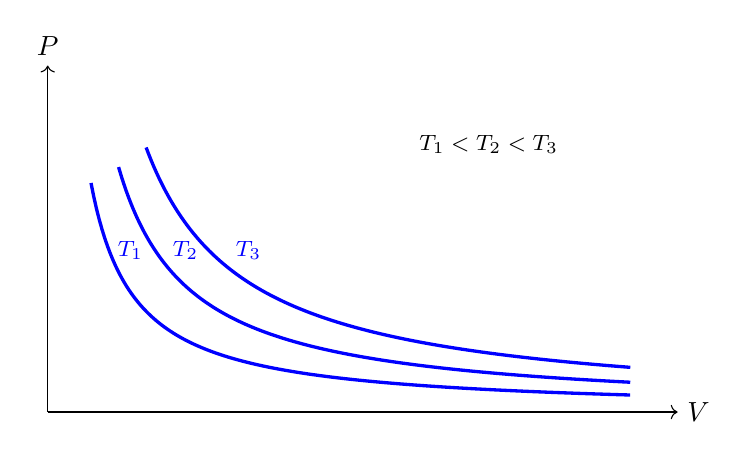
\begin{tikzpicture}[scale=1.0]
    \draw[->] (0,0) -- (8,0) node[right] {$V$};
    \draw[->] (0,0) -- (0,4.4) node[above] {$P$};

    % three isotherms P = c/V
    \draw[blue, very thick, domain=0.55:7.4, samples=200]
        plot (\x, {1.6/\x});
    \draw[blue, very thick, domain=0.9:7.4, samples=200]
        plot (\x, {2.8/\x});
    \draw[blue, very thick, domain=1.25:7.4, samples=200]
        plot (\x, {4.2/\x});

    \node[blue, font=\footnotesize] at (1.05,2.05) {$T_1$};
    \node[blue, font=\footnotesize] at (1.75,2.05) {$T_2$};
    \node[blue, font=\footnotesize] at (2.55,2.05) {$T_3$};
    \node[font=\footnotesize] at (5.6,3.4) {$T_1<T_2<T_3$};
\end{tikzpicture}
\caption{Isotherms of an ideal gas in the $P$--$V$ plane. Each curve is a
hyperbola $P = Nk_BT/V$ at fixed temperature; higher temperatures lie further
from the origin.}
\label{fig:isotherms}
\end{figure}

Let's look at a partitioned, thermally insulated box. The top partition is empty, while the bottom has a gas with temperature $T$ and pressure $P$ enclosed in a volume $V$. When we remove the partition, the gas moves up and occupies the rest of the box. In this case we have $Q=0$ and $W=0$, which means the internal energy $\Delta U$ remains the same. This means the temperature doesn't change either (since $U = \frac{3}{2}Nk_BT = \frac{3}{2}nRT$). Processes that proceed through equilibrium states are called quasi-static processes. They are not static, but are sufficiently slow that you can assume, at any point, the system is in equilibrium. (The free expansion just described is \emph{not} quasi-static, which is why you cannot draw a proper $P$--$V$ curve for it.) There is a subtle difference between a quasi-static process and a reversible process. Let's say that instead of an empty top partition we have a bunch of sand, and we take off one grain at a time. This is a quasi-static process, but is it reversible? If the piston had friction this would clearly not be reversible, because no matter how slow you moved the piston it would dissipate some heat. We can say
\begin{align*}
    \text{reversible} &\implies \text{quasi-static}\\
    \text{quasi-static} &\not\implies \text{reversible}
\end{align*}
For an isothermal process, we obtain from simple integration
\begin{align}
\begin{split}
    W &= Nk_BT\ln(V_2/V_1)\\
    Q &= W
\end{split}
\end{align}
\section{Lecture 21}
\subsection{Adiabatic process: no heat exchanged}
The situation here is a little different since $\Delta U$ is not necessarily 0 anymore. Firstly, recall, for a monatomic ideal gas 
\begin{equation*}
    U = \frac{3}{2}nRT
\end{equation*}
At constant volume $\Delta U = \delta Q$ since no work is done. This means, for one mole of a monatomic ideal gas,
\begin{equation*}
    \frac{dU}{dT} = \left(\frac{\delta Q}{\partial T}\right)_V = \frac{3}{2}R
\end{equation*}
We define the specific heat at constant volume $C_V$ to be the above quantity 
\begin{equation}
    C_V = \left(\frac{\delta Q}{\partial T}\right)_V
\end{equation}
This also means 
\begin{equation}
    dU = C_VdT
\end{equation}
If instead we took a constant pressure path, we would have to use the first law, since the work is no longer equal to zero here. 
\begin{equation*}
    \left(\pd{Q}{T}\right)_P = \frac{dU}{dT} + \frac{\delta W}{dT} = \frac{dU}{dT}+P\frac{dV}{dT} = \frac{dU}{dT}+ R = C_V+ R
\end{equation*}
So we get the important relation 
\begin{equation*}
    C_P = C_V + R
\end{equation*}
Recall, 
\begin{align*}
    \text{monatomic:}\qquad C_V = \frac{3}{2}R \implies C_P = \frac{5}{2}R\\
    \text{diatomic:}\qquad C_V = \frac{5}{2}R\implies C_P = \frac{7}{2}R\\
    \text{polyatomic:}\qquad C_V = 3R \implies C_P = 4R
\end{align*}
Now going back to the adiabatic process. We want to find the work
\begin{equation*}
    W = \int^{V_1}_{V_2}\frac{nRT}{V}dV 
\end{equation*}
but this is tough, since $T$ is changing. Instead, we use $dU = nC_V dT$. 
\begin{equation*}
    nC_V dT = -PdV = -\frac{nRT}{V}dV
\end{equation*}
Note what an adiabatic curve looks like compared to an isothermal curve.
\begin{figure}[H]
\centering
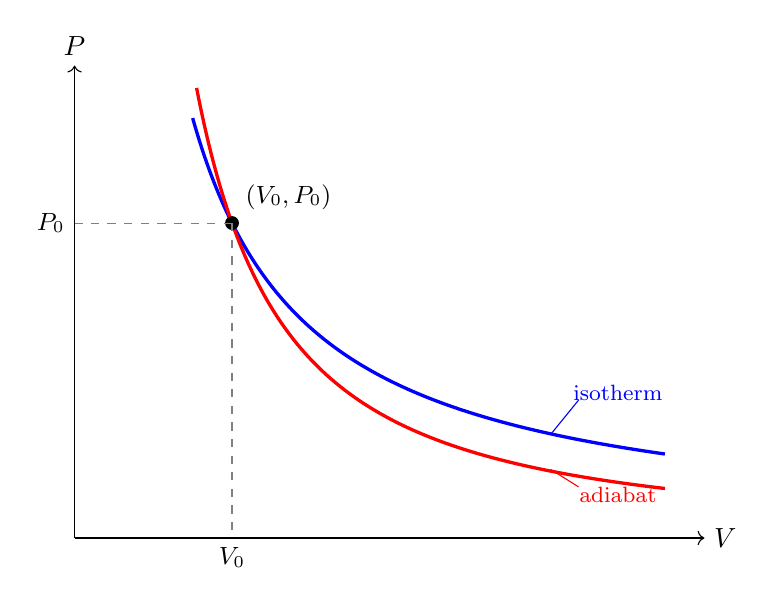
\begin{tikzpicture}[scale=1.0]
    \draw[->] (0,0) -- (8,0) node[right] {$V$};
    \draw[->] (0,0) -- (0,6) node[above] {$P$};

    % Common state (V0, P0) = (2, 4).
    % Isotherm: P = 8/V          (PV = 8)
    % Adiabat:  P = 10.556/V^1.4 (gamma = 1.4)

    % isotherm (gentler)
    \draw[blue, very thick, domain=1.5:7.5, samples=200]
        plot (\x, {8/\x});

    % adiabat (steeper)
    \draw[red, very thick, domain=1.55:7.5, samples=200]
        plot (\x, {10.556/pow(\x,1.4)});

    % shared state point with dashed projections
    \fill (2,4) circle (2.5pt);
    \node[above right, font=\small] at (2.05,4.05) {$(V_0,P_0)$};
    \draw[dashed, gray] (2,4) -- (2,0);
    \node[below, font=\small] at (2,0) {$V_0$};
    \draw[dashed, gray] (2,4) -- (0,4);
    \node[left, font=\small] at (0,4) {$P_0$};

    % curve labels with leader lines
    \node[blue, font=\footnotesize] at (6.9, 1.85) {isotherm};
    \draw[blue, thin] (6.4, 1.75) -- (6.05, 1.32);

    \node[red, font=\footnotesize] at (6.9, 0.55) {adiabat};
    \draw[red, thin] (6.4, 0.65) -- (6.05, 0.87);
\end{tikzpicture}
\caption{An isotherm (blue, $PV=\text{const.}$) and an adiabat (red, $PV^\gamma=\text{const.}$) through the same state $(V_0,P_0)$. Because $\gamma>1$, the adiabat is steeper everywhere: it lies above the isotherm for $V<V_0$ and below it for $V>V_0$.}
\label{fig:isotherm_vs_adiabat}
\end{figure}
Rearranging the above,
\begin{equation*}
    \frac{C_VdT}{T} + R\frac{dV}{V} =0 \implies C_V\ln T + R\ln V = \text{const.}
\end{equation*}
Then dividing by $C_V$, and taking the exponential
\begin{equation*}
    \ln T + \frac{R}{C_V}\ln V = \text{const.} \implies TV^{\frac{R}{C_V}} = \text{another const.}
\end{equation*}
Now we introduce $\gamma = \frac{C_P}{C_V} = 1 + \frac{R}{C_V}$. So we can write the above as 
\begin{equation}
    TV^{\gamma - 1} = \text{const.}
\end{equation}
Since $PV = nRT$, 
\begin{equation}
    PV^{\gamma} = \text{const.}
\end{equation}
We see that all the adiabatic process curves are steeper than the isothermal process curves. Now we can ask what the work is given by in an adiabatic process. 
\begin{align*}
    \delta W = PdV \qquad P = \frac{\text{C}}{V^{\gamma}}\\
    W = \int^{V_2}_{V_1}\frac{C}{V^{\gamma}}dV = C\frac{V^{1-\gamma}}{1-\gamma}\bigg|^{V_2}_{V_1} = \frac{C}{1-\gamma}\left(V_2^{1-\gamma}-V_1^{1-\gamma}\right)
\end{align*}
Since $C+ P_1V_1^{\gamma} = P_2V_2^{\gamma}$, some algebra gives us 
\begin{equation}
    W = \frac{P_2V_2 - P_1V_1}{1-\gamma}
\end{equation}
We can do this another way. In an adiabatic process 
\begin{equation*}
    \delta W = -dU = -C_VdT \implies W = -C_V(T_2 -T_1) = C_V(T_1-T_2)
\end{equation*}
To see this is equivalent to the previous expression of work, let's look at one mole and work towards our newer answer, 
\begin{equation*}
    W = \frac{P_2V_2 -P_1V_1}{1-\gamma} = \frac{RT_2 - RT_1}{1-\gamma} = \frac{R}{1-\gamma}(T_2-T_1)
\end{equation*}
Now we can check that $-C_V = \frac{R}{1-\gamma}$. 
\begin{align*}
    -C_V = \frac{R}{1-\gamma} \implies -C(1-\gamma) = R\\
    \gamma = \frac{C_P}{C_V} = 1+\frac{R}{C_V} \implies -C_V(1-1-\frac{R}{C_V}) = R 
\end{align*}
So the equivalnce is there. The rest of this lecture is on cycles. I have not included them here because they are best learnt by doing problems.
\section{Lecture 22}
Let's talk about a cycle that will lead us to the second law of thermodynamics. We have an isothermal process from $A$ to $B$, an adiabatic process from $B$ to $C$, an isothermal process from $C$ to $D$, and finally an adiabatic process bringing us back from $D$ to $A$. This is the \textbf{Carnot cycle}.

\begin{figure}[H]
\centering
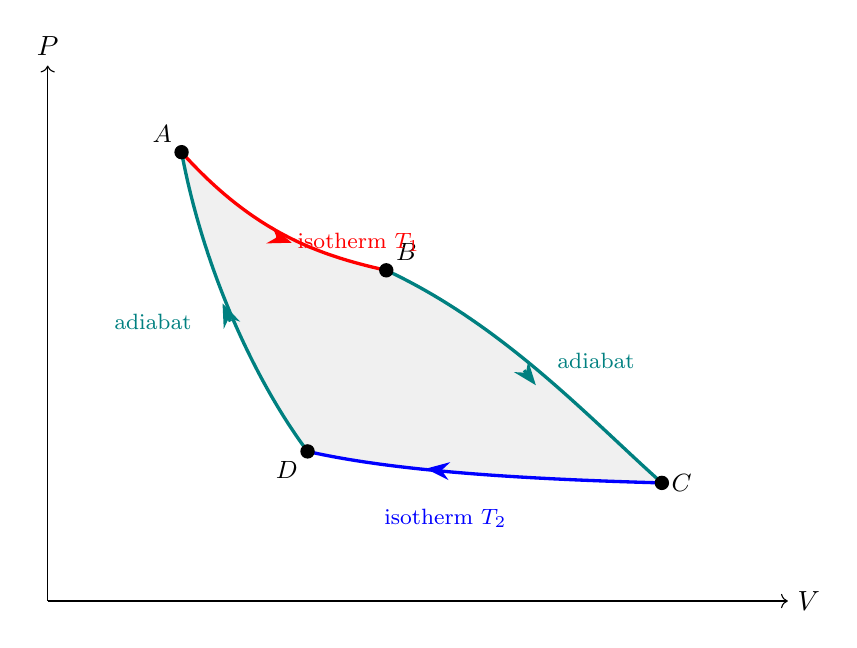
\begin{tikzpicture}[scale=1.0]
    \draw[->] (0,0) -- (9.4,0) node[right] {$V$};
    \draw[->] (0,0) -- (0,6.8) node[above] {$P$};

    \coordinate (A) at (1.7,5.7);
    \coordinate (B) at (4.3,4.2);
    \coordinate (C) at (7.8,1.5);
    \coordinate (D) at (3.3,1.9);

    \fill[gray!12]
        (A) .. controls (2.6,4.7) and (3.4,4.4) .. (B)
        .. controls (5.8,3.5) and (6.9,2.3) .. (C)
        .. controls (6.0,1.55) and (4.4,1.65) .. (D)
        .. controls (2.7,2.7) and (2.0,4.1) .. (A) -- cycle;

    \draw[red, very thick]
        (A) .. controls (2.6,4.7) and (3.4,4.4) .. (B);
    \draw[teal, very thick]
        (B) .. controls (5.8,3.5) and (6.9,2.3) .. (C);
    \draw[blue, very thick]
        (C) .. controls (6.0,1.55) and (4.4,1.65) .. (D);
    \draw[teal, very thick]
        (D) .. controls (2.7,2.7) and (2.0,4.1) .. (A);

    \draw[red,  very thick, -{Stealth[length=3mm]}] (2.9,4.62) -- (3.1,4.55);
    \draw[teal, very thick, -{Stealth[length=3mm]}] (6.05,2.93) -- (6.2,2.74);
    \draw[blue, very thick, -{Stealth[length=3mm]}] (5.0,1.66) -- (4.8,1.68);
    \draw[teal, very thick, -{Stealth[length=3mm]}] (2.32,3.55) -- (2.22,3.78);

    \fill (A) circle (2.6pt); \node[above left,  font=\small] at (A) {$A$};
    \fill (B) circle (2.6pt); \node[above right, font=\small] at (B) {$B$};
    \fill (C) circle (2.6pt); \node[right,       font=\small] at (C) {$C$};
    \fill (D) circle (2.6pt); \node[below left,  font=\small] at (D) {$D$};

    \node[red,  font=\footnotesize] at (3.95,4.55) {isotherm $T_1$};
    \node[blue, font=\footnotesize] at (5.05,1.05) {isotherm $T_2$};
    \node[teal, font=\footnotesize, right] at (6.35,3.05) {adiabat};
    \node[teal, font=\footnotesize, left]  at (1.95,3.55) {adiabat};
\end{tikzpicture}
\caption{The Carnot cycle. Two isotherms (at temperatures $T_1$ and $T_2$, with $T_1>T_2$) joined by two adiabats, traversed clockwise so that net work is done by the gas.}
\label{fig:carnot_intro}
Let $Q_1$ be the heat absorbed in the process from $A$ to $B$ and $Q_2$ the heat \textbf{released} in the process from $C$ to $D$ (we change the convention here such that $Q_2>0$). We know, 
\begin{align*}
    Q_1 = Q_{AB} = W_{AB} = nRT_1\ln\frac{V_B}{V_A}\\
    -Q_2 = Q_{CD} = W_{CD} = nRT_2\ln\frac{V_D}{V_C}
\end{align*}
\end{figure}
Since the volume at $D$ is smaller than the volume at $C$, the logarithm is negative and so the heat is positive. Since the other two processes are adiabatic, there is no heat exchange. So the total heat is given by 
\begin{equation}
    Q_{tot} = nRT_1\ln\frac{V_B}{V_A} + nRT_2\ln\frac{V_C}{V_D}
\end{equation}
By the first law, since we are in a cycle $\Delta U = 0$. 
\begin{equation*}
    W_{BC} + W_{DA} = C_V(T_1-T_2) + C_V(T_2-T_1) = 0
\end{equation*}
The total work on the cycle is given also by $W = Q_1-Q_2$ (absorbed - released). What we have done here is converted heat into work, but not all of the heat was converted into work. This here is a heat engine. 
The efficieny is naturally defined as 
\begin{equation}
    \eta = \frac{W}{Q_1} = \frac{Q_1 - Q_2}{Q_1} = 1 -\frac{Q_2}{Q_1}
\end{equation}
The second law of thermodynamcis says that $\eta <1$. Note that 
\begin{align*}
    \frac{Q_2}{Q_1} = \frac{T_2}{T_1}\frac{\ln\frac{V_C}{V_D}}{\ln \frac{V_B}{V_A}}
\end{align*}
and also 
\begin{align*}
    T_1V_B^{\gamma -1} = T_2V_C^{\gamma -1}\\
    T_1V_A^{\gamma -1} = T_2V_D^{\gamma - 1}\\
    \implies \left(\frac{V_B}{B_A}\right) = \left(\frac{V_C}{V_D}\right)\\
    \implies \frac{Q_2}{Q_1} = \frac{T_2}{T_1}
\end{align*}
We can consider any other cycle and do the same analysis. For a generic Heat engine. We have a heat reservoir. We then have our ideal gas which we call our ideal gas. There is heat going into the heat engine, and then heat going out of it going into a reservoir $T_2$. There is some work done by the difference in work. 
The efficiency $\eta = 1 - \frac{T_2}{T_1}$ is general. Note that $T_2<T_1$. The heat engine undergoes a cycle, so we can assume $\Delta U = 0$. That is what makes $W = Q_1 - Q_2$ valid. The reverse of this is known as the \textbf{refrigerator}. Here we have the same reservoirs, with $Q_2$ coming out of the lower temperature and going into the $Q_1$ into the higher temperature. We put work into the system here
\subsection{The Second Law of Thermodynamics}
The first law says energy is conserved. If we have some body that drops to the ground. When it hits the ground it gets hotter, because of the motion in the molecules in the body. We will not see the ball go back up to the same height, but this is not forbidden by the first law, so we need a second law. 
This is an example of an \textbf{irreversible process}. The Carnot cycle we have been speaking about is a reversible process.  There are two statements of the second law. The first statement, called the \textbf{Kelvin-Planck} statement says 
\begin{center}
    You cannot build an engine whose sole effect is to turn heat into work. 
\end{center}
This just says you must have a $Q_2$. The second statement, the \textbf{Clausius} statement, says
\begin{center}
    You can't transfer heat from a cold body to a hotter body without work
\end{center}
These two statements are equivalent. A consequence is that 
\begin{equation}
    \frac{Q_1}{T_1} - \frac{Q_2}{T_2} < 0
\end{equation}
We can define the change in entropy as 
\begin{equation}
    \Delta S = \frac{Q}{T}
\end{equation}
or in the differential form 
\begin{equation}
    dS = \frac{\delta Q}{T}
\end{equation}
The total change in entropy in the carnot cycle is 
\begin{equation}
    \Delta S_{\text{carnot}} = \Delta S_{AB} + \Delta S_{CD} = \frac{Q_1}{T} + \frac{(-Q)}{T_2} = 0
\end{equation}
Entropy is a function of state. 
\section{Lecture 23}
\subsection{Entropy and the 2nd Law continued}
\begin{equation}
    \Delta S \geq 0
\end{equation}

The entropy $S$ is mathematically defined as
\begin{equation}
    \Delta S = S_b - S_a = \int^b_a \frac{\delta Q}{T}
\end{equation}
Where $a,b$ are states and the integral is taken along a \emph{reversible} process. Also note that
\begin{equation*}
    \delta Q = \text{heat absorbed by the system}
\end{equation*}
where the process is reversible. Say you have a box with a partition, where one side is empty and the other is filled with particles. You remove the partition and the particles fill up the whole container. If the
box is insulated and the gas is ideal, no heat crosses the boundary, so $\delta Q = 0$ along the actual path. It is tempting to conclude $\Delta S = 0$ -- but this is wrong, because $\Delta S = \int\delta Q/T$ only along a \emph{reversible} path, and free expansion is irreversible. \textbf{Entropy is a function of state}, so we may still compute $\Delta S$ by constructing a reversible process connecting the same two endpoints.\\

\noindent Recall that for an isothermal process where the volume gets larger, we can compute the change in heat from the first law
\begin{align*}
    \delta W &= P\, dV = \delta Q\\
    \implies \int^b_a \frac{P\, dV}{T} &= \int^{V_2}_{V_1}\frac{nR\,\cancel T}{V\,\cancel T}dV = nR\ln \frac{V_2}{V_1} = S(T,V_2) - S(T,V_1)
\end{align*}
Now we can ask the more general question. What is $S(T,V)$ for an ideal gas? Say we have an isotherm that goes through $a$, and another isotherm that goes through $b$. How do you compute the entropy difference between $a$ and $b$?
\section{Lecture 24}
\subsection{Entropy, ideal gas (continued)}
Recall that, in a reversible process,
\begin{equation*}
    dS = \frac{\delta Q}{T}.
\end{equation*}
Then the change in entropy is given by
\begin{equation*}
    \Delta S = S_b - S_a = \int^b_a \frac{\delta Q}{T}
\end{equation*}
where $a$ to $b$ is a reversible path and $\delta Q$ is the heat absorbed by the system. Applying this general definition to an ideal gas, as we did last lecture, we find for an initial state $(P_1,V_1)$ and final state $(P_2,V_2)$ that
\begin{equation*}
    \Delta S_{12} = S_2 - S_1.
\end{equation*}
If we have an isothermal process from 1 to 3, and then a constant volume process from 3 to 2 (so that 3 lies at the final volume, $V_3 = V_2$),
\begin{equation*}
    \Delta S_{13} = \int^3_1 \frac{\delta Q}{T} = \int^{V_3}_{V_1} \frac{nRT}{VT}dV = nR \ln\frac{V_3}{V_1}
\end{equation*}
The heat here is going into the system, since we are performing positive work in an isothermal expansion. Then, the entropy from 3 to 2 (where $\delta W = 0$ since volume is constant, which means $\delta Q = dU = nc_v\, dT$) is given by
\begin{equation*}
    \Delta S_{32} = S_2 - S_3 = \int^{T_2}_{T_1}\frac{nc_v\, dT}{T} = nc_v\ln \frac{T_2}{T_1}
\end{equation*}
Keeping it general,
\begin{equation*}
    \Delta S_{12} = nR\ln\frac{V_2}{V_1}+nc_v\ln\frac{T_2}{T_1}
\end{equation*}
This should be true for any arbitrary path from 1 to 2. Take another path $B$. $B$ starts with an expansion at constant pressure, then a decrease in pressure at constant volume. From the first law of thermodynamics, the first part of this
path is given by $\delta Q = dU + \delta W = nc_p\, dT$, where $c_p = c_v + R$. This is a result we derived earlier. Let the first leg run from 1 to $3'$. Then,
\begin{equation*}
    \Delta S_{13'} = \int^{T_{3'}}_{T_1}\frac{nc_p\, dT}{T}= nc_p\ln\frac{T_{3'}}{T_1}
\end{equation*}
Now from $3'$ to $2$, we have a constant volume process, which implies $dU = \delta Q$. So,
\begin{equation*}
    \Delta S_{3'2} = \int^{T_2}_{T_{3'}}nc_v\frac{dT}{T} = nc_v\ln\frac{T_2}{T_{3'}}
\end{equation*}
Then,
\begin{equation*}
    \Delta S^B_{12} = nc_p\ln\frac{T_{3'}}{T_1} + nc_v\ln\frac{T_2}{T_{3'}}
\end{equation*}

\begin{figure}[H]
\centering
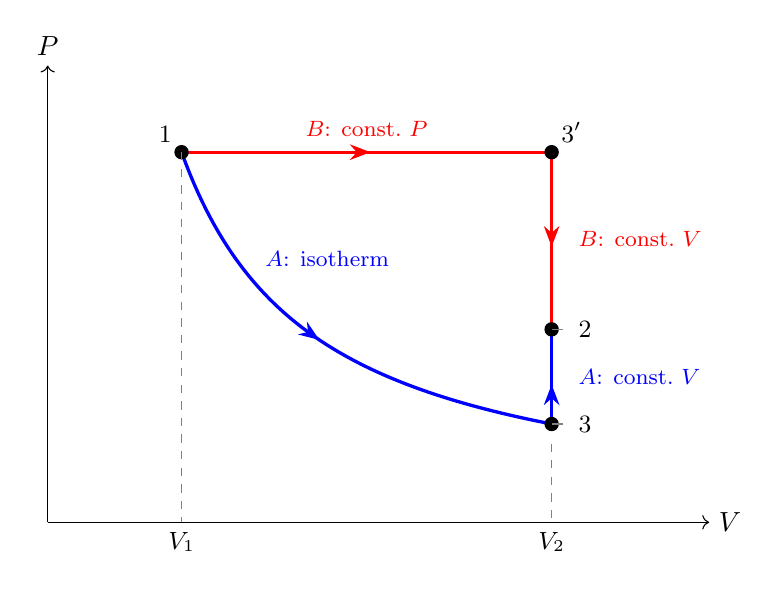
\begin{tikzpicture}[scale=1.0]
    % axes
    \draw[->] (0,0) -- (8.4,0) node[right] {$V$};
    \draw[->] (0,0) -- (0,5.8) node[above] {$P$};

    % volume gridlines
    \node[below, font=\small] at (1.7,0) {$V_1$};
    \node[below, font=\small] at (6.4,0) {$V_2$};

    % state points. 1 high-left, 3' at same P as 1 and V=V2,
    % 2 below 3', 3 on the isotherm through 1 at V=V2 (lowest).
    \coordinate (S1)  at (1.7,4.7);
    \coordinate (S3p) at (6.4,4.7);   % const-P leg of B ends here (P = P1)
    \coordinate (S2)  at (6.4,2.45);  % final state
    \coordinate (S3)  at (6.4,1.248); % isotherm thru 1 at V2: P1 V1 / V2 = 4.7*1.7/6.4

    % ;- path A (blue): isotherm 1 -> 3, then constant volume 3 -> 2 ;-
    \draw[blue, very thick, domain=1.7:6.4, samples=90]
        plot (\x, {4.7*1.7/\x});            % isotherm 1 -> 3
    \draw[blue, very thick] (S3) -- (S2);    % const V: 3 -> 2
    % arrows for A
    \draw[blue, very thick, -{Stealth[length=2.6mm]}]
        (3.3,{7.99/3.3}) -- (3.45,{7.99/3.45});
    \draw[blue, very thick, -{Stealth[length=2.6mm]}]
        (6.4,1.55) -- (6.4,1.75);

    % ;- path B (red): constant pressure 1 -> 3', then constant volume 3' -> 2 ;-
    \draw[red, very thick] (S1) -- (S3p);    % const P: 1 -> 3'
    \draw[red, very thick] (S3p) -- (S2);    % const V: 3' -> 2
    % arrows for B
    \draw[red, very thick, -{Stealth[length=2.6mm]}] (3.9,4.7) -- (4.1,4.7);
    \draw[red, very thick, -{Stealth[length=2.6mm]}] (6.4,3.7) -- (6.4,3.5);

    % state markers
    \fill (S1)  circle (2.6pt); \node[above left,  font=\small] at (S1)  {$1$};
    \fill (S3p) circle (2.6pt); \node[above right, font=\small] at (S3p) {$3'$};
    \fill (S2)  circle (2.6pt);
    \fill (S3)  circle (2.6pt);

    % leg labels (placed clear, with leader lines where needed)
    \node[red,  font=\footnotesize, above] at (4.05,4.78) {$B$: const.\ $P$};
    \node[blue, font=\footnotesize] at (3.55,3.35) {$A$: isotherm};

    % "const. V" labels and the 2 / 3 point labels off to the right
    \node[red,  font=\footnotesize, right] at (6.62,3.6) {$B$: const.\ $V$};
    \node[blue, font=\footnotesize, right] at (6.62,1.85) {$A$: const.\ $V$};
    \node[font=\small, right] at (6.62,2.45) {$2$};
    \node[font=\small, right] at (6.62,1.248) {$3$};
    \draw[gray] (6.55,2.45) -- (6.4,2.45);
    \draw[gray] (6.55,1.248) -- (6.4,1.248);

    % dashed volume projections
    \draw[dashed, gray] (S1) -- (1.7,0);
    \draw[dashed, gray] (6.4,1.0) -- (6.4,0);
\end{tikzpicture}
\caption{Two reversible paths between the same states $1$ and $2$ in the
$P$--$V$ plane. Path $A$ (blue) is an isotherm $1\to3$ followed by a
constant-volume leg $3\to2$; path $B$ (red) is a constant-pressure leg
$1\to3'$ followed by a constant-volume leg $3'\to2$. Both constant-volume
legs lie on $V=V_2$. The entropy change $\Delta S_{12}$ is the same along
either path, because $S$ is a function of state.}
\label{fig:entropy_paths}
\end{figure}

Now how do we show this is equivalent to path $A$? Note that
\begin{equation}
    nc_p\ln\frac{T_{3'}}{T_1}= nc_v\ln\frac{T_{3'}}{T_1}+nR\ln\frac{T_{3'}}{T_1}
\end{equation}
So we get
\begin{equation*}
    \Delta S^B_{12} = nc_v\ln\frac{T_{3'}}{T_1}+nR\ln\frac{T_{3'}}{T_1} + nc_v\ln\frac{T_2}{T_{3'}}=nc_v\ln\frac{T_2}{T_1}+nR\ln\frac{T_{3'}}{T_1}
\end{equation*}
Since $3'$ is at $(P_1,V_2)$, we get that $T_{3'} = \frac{P_1V_2}{nR}$, and $T_1 = \frac{P_1V_1}{nR}$, which means $\frac{T_{3'}}{T_1} = \frac{V_2}{V_1}$. This gives us the desired result. Now we can get this result without annoying calculations, and we can show that it is independent of the path taken. From the first law
\begin{equation}
    dU = \delta Q - \delta W = T\,dS - P\,dV.
\end{equation}
Note that $\delta Q$ is not a function of state -- it is an inexact differential. But $dS = \delta Q/T$ \emph{is} an exact differential. From this equation, we can write
\begin{equation*}
    dS = \frac{1}{T} dU + \frac{P}{T}dV.
\end{equation*}
Now this is an exact differential, and we can integrate it along any path. Recall,
\begin{equation*}
    \Delta S = S_2 - S_1 = \underset{\text{any path}}{\int}dS = \int\left(\frac{1}{T}dU+\frac{P}{T}dV\right)= \int^2_1\left(\frac{nc_v}{T}dT + \frac{nR}{V}dV\right)=nc_v\ln\frac{T_2}{T_1}+nR\ln\frac{V_2}{V_1}
\end{equation*}
So we get the same result without specifying anything about the path. We should be specific and say that this is true not for any path but for any reversible path. Now we ask the more interesting question: how do you find the change in entropy
between two states if the process between them is irreversible? The solution is to construct a reversible process (or processes) that connect the two states.
\subsection{Heat engines} We have a cycle where heat $Q_1$ goes into the engine and $Q_2$ comes out of the engine, with reservoir temperatures $T_1$ and $T_2$. We defined the efficiency to be
\begin{equation*}
    \eta = \frac{W}{Q_1} = \frac{Q_1 - Q_2}{Q_1}
\end{equation*}
where $W = Q_1 - Q_2$ because the internal energy doesn't change over a cycle. For a Carnot cycle, we found that
\begin{equation*}
    \eta = 1 - \frac{T_2}{T_1} \implies \frac{Q_2}{Q_1} = \frac{T_2}{T_1}
\end{equation*}

\begin{figure}[H]
\centering
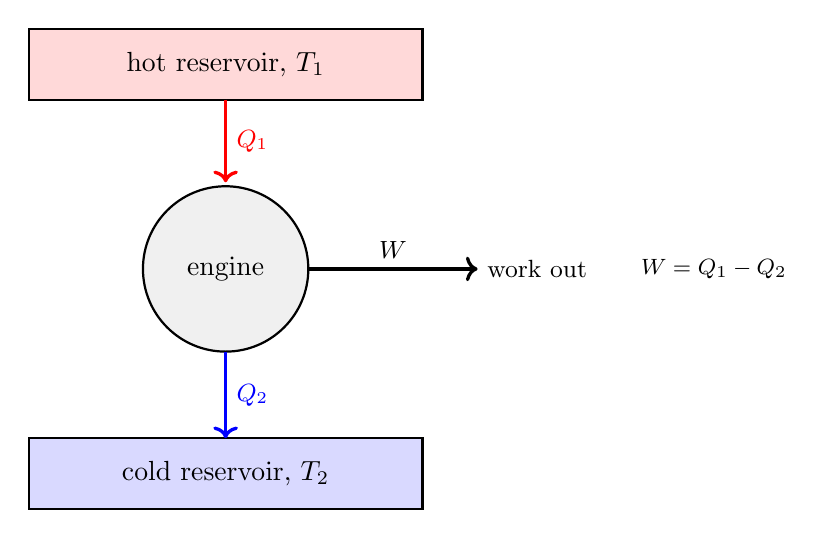
\begin{tikzpicture}[scale=1.0]

    % hot reservoir
    \draw[thick, fill=red!15] (0,3.6) rectangle (5,4.5);
    \node at (2.5,4.05) {hot reservoir, $T_1$};

    % cold reservoir
    \draw[thick, fill=blue!15] (0,-1.6) rectangle (5,-0.7);
    \node at (2.5,-1.15) {cold reservoir, $T_2$};

    % engine
    \draw[thick, fill=gray!12] (2.5,1.45) circle (1.05);
    \node at (2.5,1.45) {engine};

    % Q1 in (hot reservoir -> engine)
    \draw[->, very thick, red] (2.5,3.6) -- (2.5,2.55)
        node[midway, right, font=\small] {$Q_1$};
    % Q2 out (engine -> cold reservoir)
    \draw[->, very thick, blue] (2.5,0.4) -- (2.5,-0.7)
        node[midway, right, font=\small] {$Q_2$};

    % W out
    \draw[->, very thick] (3.55,1.45) -- (5.7,1.45)
        node[midway, above, font=\small] {$W$};
    \node[right, font=\small] at (5.7,1.45) {work out};

    % energy balance note
    \node[font=\footnotesize] at (8.7,1.45) {$W = Q_1 - Q_2$};

\end{tikzpicture}
\caption{Block diagram of a heat engine. Over one cycle the engine absorbs
heat $Q_1$ from the hot reservoir, rejects $Q_2$ to the cold reservoir, and
delivers work $W = Q_1 - Q_2$. The efficiency is $\eta = W/Q_1$, and for a
Carnot engine $\eta = 1 - T_2/T_1$.}
\label{fig:heat_engine}
\end{figure}

The Carnot cycle is the prototype reversible cycle: two isotherms (at $T_1$ and
$T_2$) joined by two adiabats. In the $P$--$V$ plane it is a closed loop, and the
area enclosed is the net work $W$ done per cycle.

\begin{figure}[H]
\centering
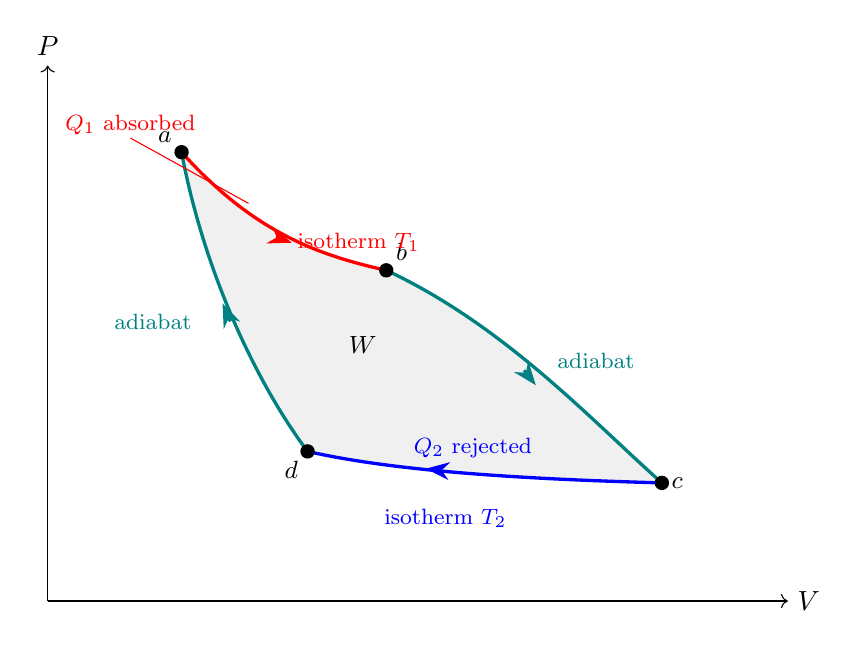
\begin{tikzpicture}[scale=1.0]
    % axes
    \draw[->] (0,0) -- (9.4,0) node[right] {$V$};
    \draw[->] (0,0) -- (0,6.8) node[above] {$P$};

    % ; Carnot loop drawn schematically as four distinct arcs ;
    % Corners chosen well-separated so the enclosed area is clearly visible.
    \coordinate (a) at (1.7,5.7);   % top-left
    \coordinate (b) at (4.3,4.2);   % upper-right-ish
    \coordinate (c) at (7.8,1.5);   % bottom-right
    \coordinate (d) at (3.3,1.9);   % lower-left-ish

    % shaded interior
    \fill[gray!12]
        (a) .. controls (2.6,4.7) and (3.4,4.4) .. (b)
        .. controls (5.8,3.5) and (6.9,2.3) .. (c)
        .. controls (6.0,1.55) and (4.4,1.65) .. (d)
        .. controls (2.7,2.7) and (2.0,4.1) .. (a) -- cycle;

    % isotherm T1 : a -> b  (gentle arc, bows down only slightly)
    \draw[red, very thick]
        (a) .. controls (2.6,4.7) and (3.4,4.4) .. (b);
    % adiabat : b -> c  (steeper arc)
    \draw[teal, very thick]
        (b) .. controls (5.8,3.5) and (6.9,2.3) .. (c);
    % isotherm T2 : c -> d  (gentle arc)
    \draw[blue, very thick]
        (c) .. controls (6.0,1.55) and (4.4,1.65) .. (d);
    % adiabat : d -> a  (steep arc)
    \draw[teal, very thick]
        (d) .. controls (2.7,2.7) and (2.0,4.1) .. (a);

    % direction arrows (clockwise a->b->c->d->a)
    \draw[red,  very thick, -{Stealth[length=3mm]}] (2.9,4.62) -- (3.1,4.55);
    \draw[teal, very thick, -{Stealth[length=3mm]}] (6.05,2.93) -- (6.2,2.74);
    \draw[blue, very thick, -{Stealth[length=3mm]}] (5.0,1.66) -- (4.8,1.68);
    \draw[teal, very thick, -{Stealth[length=3mm]}] (2.32,3.55) -- (2.22,3.78);

    % state markers
    \fill (a) circle (2.6pt); \node[above left,  font=\small] at (a) {$a$};
    \fill (b) circle (2.6pt); \node[above right, font=\small] at (b) {$b$};
    \fill (c) circle (2.6pt); \node[right,       font=\small] at (c) {$c$};
    \fill (d) circle (2.6pt); \node[below left,  font=\small] at (d) {$d$};

    % leg labels
    \node[red,  font=\footnotesize] at (3.95,4.55) {isotherm $T_1$};
    \node[blue, font=\footnotesize] at (5.05,1.05) {isotherm $T_2$};
    \node[teal, font=\footnotesize, right] at (6.35,3.05) {adiabat};
    \node[teal, font=\footnotesize, left]  at (1.95,3.55) {adiabat};

    % heat-flow annotations
    \node[red,  font=\footnotesize] at (1.05,6.05) {$Q_1$ absorbed};
    \draw[red] (1.05,5.88) -- (2.55,5.05);
    \node[blue, font=\footnotesize] at (5.4,1.95) {$Q_2$ rejected};
    \node[font=\small] at (4.0,3.25) {$W$};
\end{tikzpicture}
\caption{The Carnot cycle in the $P$--$V$ plane, drawn schematically with the
adiabats steeper than the isotherms. Isothermal expansion $a\!\to\!b$ at $T_1$
absorbs heat $Q_1$; adiabatic expansion $b\!\to\!c$; isothermal compression
$c\!\to\!d$ at $T_2$ rejects heat $Q_2$; adiabatic compression $d\!\to\!a$
closes the loop. The shaded enclosed area is the net work $W = Q_1 - Q_2$
done per cycle.}
\label{fig:carnot_cycle}
\end{figure}

We didn't quite prove that any reversible engine operating between the given temperatures $T_1$ and $T_2$ has the same efficiency (same $\frac{Q_2}{Q_1}$). This is a nontrivial statement. We can show that if it were not true, it would violate either the Clausius or Kelvin statements of the second law.
We have been assuming $Q_1>0, Q_2>0$. But recall how we defined heat absorption; if we redefine $Q_2\rightarrow -Q_2$ so that all heats are counted as absorbed by the system, then we get
\begin{equation}
    \frac{Q_1}{T_1} + \frac{Q_2}{T_2} = 0 \implies \oint_C \frac{\delta Q}{T} =0
\end{equation}
where $C$ is a reversible cycle. There are two ways to prove this. First, we look at any cycle as the superposition of Carnot cycles. You can keep constructing Carnot cycles that tile our arbitrary cycle, and we sum them up. All the internal pieces cancel out since the heats are of opposite signs along shared edges, so we are left with just the boundary. So we obtain
\begin{equation}
    \sum_{\text{Carnot cycles}}\frac{Q_i}{T_i} =\oint_C\frac{\delta Q}{T}
\end{equation}

\begin{figure}[H]
\centering
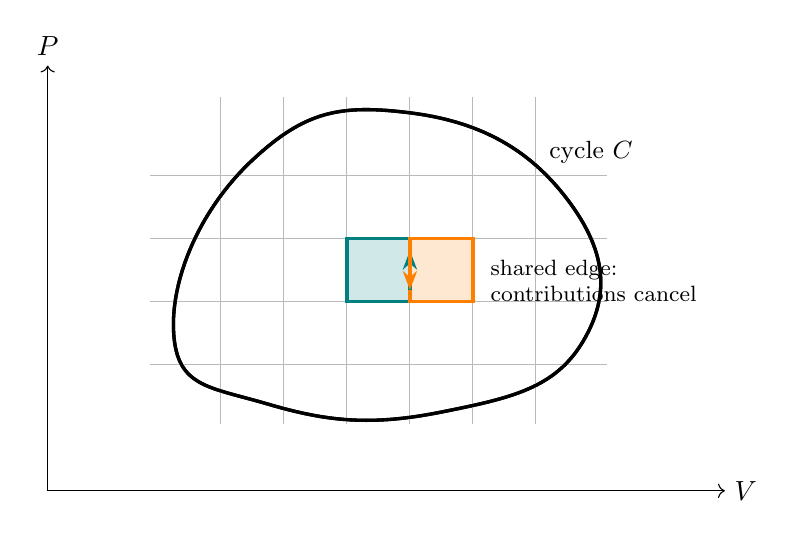
\begin{tikzpicture}[scale=1.0]
    % axes
    \draw[->] (0,0) -- (8.6,0) node[right] {$V$};
    \draw[->] (0,0) -- (0,5.4) node[above] {$P$};

    % an arbitrary smooth reversible cycle C (a closed blob)
    \draw[very thick, black]
        plot[smooth cycle, tension=0.8]
        coordinates {(1.6,2.0) (2.6,4.2) (4.6,4.8) (6.6,3.7)
                     (6.8,1.9) (5.0,1.0) (2.8,1.1)};
    \node[font=\small] at (6.9,4.3) {cycle $C$};

    % grid of thin Carnot tiles (isotherms horizontal-ish, adiabats vertical-ish)
    % vertical-ish lines (adiabats)
    \foreach \x in {2.2,3.0,3.8,4.6,5.4,6.2}{
        \draw[gray!55, thin] (\x,0.85) -- (\x,5.0);
    }
    % horizontal-ish lines (isotherms)
    \foreach \y in {1.6,2.4,3.2,4.0}{
        \draw[gray!55, thin] (1.3,\y) -- (7.1,\y);
    }

    % highlight one interior tile and its neighbour to show edge cancellation
    \fill[teal!18] (3.8,2.4) rectangle (4.6,3.2);
    \fill[orange!18] (4.6,2.4) rectangle (5.4,3.2);
    \draw[teal,   very thick] (3.8,2.4) rectangle (4.6,3.2);
    \draw[orange, very thick] (4.6,2.4) rectangle (5.4,3.2);

    % opposing arrows on the shared edge
    \draw[teal,   very thick, -{Stealth[length=2.4mm]}] (4.6,2.55) -- (4.6,3.05);
    \draw[orange, very thick, -{Stealth[length=2.4mm]}] (4.6,3.05) -- (4.6,2.55);
    \node[font=\footnotesize, right] at (5.5,2.8) {shared edge:};
    \node[font=\footnotesize, right] at (5.5,2.5) {contributions cancel};

    % redraw the cycle boundary on top so it stays visible
    \draw[very thick, black]
        plot[smooth cycle, tension=0.8]
        coordinates {(1.6,2.0) (2.6,4.2) (4.6,4.8) (6.6,3.7)
                     (6.8,1.9) (5.0,1.0) (2.8,1.1)};
\end{tikzpicture}
\caption{Tiling an arbitrary reversible cycle $C$ by small Carnot cycles, each
bounded by a pair of adiabats and a pair of isotherms. Every interior edge is
traversed twice in opposite directions (teal vs.\ orange), so those
contributions to $\sum Q_i/T_i$ cancel; only the boundary survives, giving
$\sum_i Q_i/T_i = \oint_C \delta Q/T$.}
\label{fig:carnot_tiling}
\end{figure}

The second way to prove it is to construct a cycle together with a reservoir at $T_0$. If we look at a small part of the cycle, we get a change in heat (which may be absorption or release) of $\delta Q_i$. Recall that a refrigerator is the reverse of a heat engine: we put work into the cycle to move heat. Let's say we have a Carnot refrigerator that delivers heat from $T_0$ of amount $\delta Q_{0i}$ to the segment, which exchanges $\delta Q_i$ at temperature $T_i$. For a Carnot refrigerator,
\begin{equation*}
    \frac{\delta Q_{0i}}{T_0} = \frac{\delta Q_i}{T_i}
\end{equation*}
We sum it up and get
\begin{equation*}
    \sum_i \frac{\delta Q_{0i}}{T_0} = \sum_i \frac{\delta Q_i}{T_i} \implies \frac{Q_0}{T_0} = \oint \frac{\delta Q}{T}
\end{equation*}
We are trying to show that the integral must be zero. If $Q_0>0$, we put net heat into the system; by conservation of energy, since we returned to our original state, all of that heat was converted into work. This violates the Kelvin statement (you cannot have a cyclic process whose sole effect is to take in heat and convert it entirely into work). If $Q_0<0$, running everything in reverse gives the same contradiction. Hence $\oint_C\delta Q/T = 0$.
\section{Lecture 25}
\subsection{Irreversible processes}
Recall that 
\begin{equation*}
    \eta = \frac{W}{Q_1} = 1 - \frac{T_2}{T_1}
\end{equation*}
This is the upper limit of the efficiency for a reversible process. By the first law $W = Q_1 - W_2$, so $\eta = 1 - \frac{Q_2}{Q_1}$. Let the work in an irreversible process be $W'$. It follows that $W'<W$. Since $W' = Q_1 - Q_2'$, it follows that $Q_2'<Q_2$. 
In a reversible process
\begin{equation*}
    \frac{Q_1}{T_1} - \frac{Q_2}{T_2} = 0
\end{equation*}
We changed the convention to get 
\begin{equation*}
    \frac{Q_1}{T_1} + \frac{Q_2}{T_2} = 0
\end{equation*}
For an irreversible process, 
\begin{equation}
    \frac{Q_1}{T_1} + \frac{Q_2'}{T_2} < 0
\end{equation}
Remember that $Q_2$ and $Q_2'$ are both less than zero since heat is released. We can generalize further. Similar to the reversible cycle, we can obtain 
\begin{equation*}
    \oint \frac{\delta Q}{T} \leq 0 \qquad \text{(Clausius' Inequality)}
\end{equation*}
where we have equality in a reversible process and less than $0$ in an irreversible process. Let's say we have some irreversible cycle where we choose a path $a$ to b that is irreversible and a path $b$ to $a$ that is reversible. then 
\begin{equation*}
    \oint \frac{\delta Q}{T}=\underset{irreversible}{\int^b_a \frac{\delta Q}{T}} + \underset{reversible}{\int^a_b\frac{\delta Q}{T}} \leq 0
\end{equation*}
Recall that, by definition, 
\begin{equation*}
    \underset{reversible}{\int^b_a\frac{\delta Q}{T}} = S_b - S_a
\end{equation*}
Then we can rearrange the above to get
\begin{equation}
    S_b - S_a > \underset{irrev}{\int^b_a\frac{\delta Q}{T}}
\end{equation}
The right hand side is equal to $0$ for a closed system (like the universe). So we have just shown that for any process that can occure in nature, the change in entropy must be greater than $0$. The entropy can only increase. Clausius said that we cannot transfer heat from somthing cold to something hot. We can show that by computing the change in entropy 
\begin{equation*}
    \frac{-Q}{T_c} + \frac{Q}{T_h}
\end{equation*}
this is obvious less than $0$ since $T_c<T_h$. The Kelvin-Planck statement says that you cannot have a process where you turn heat into only work. Here the change in entropy is
\begin{equation*}
    S_b - S_a = -\frac{Q}{T_1} < 0 
\end{equation*}
because the cycle does not contribute to the entropy, so the only contributing factor is the heat being released by the reservoir. Let's look at a more general case of heat transfer, where two boxes at $T_1$ and $T_2$ respectively are connected and end up at some temperature $T_f$. The first law tells us that 
\begin{equation*}
    C_1(T_1-T_f) + C_2(T_2-T_f) = 0
\end{equation*}
where $C_1$ and $C_2$ are the heat capacities of the boxes. Then 
\begin{equation*}
    T_f = \frac{C_1T_1 + C_2T_2}{C_1+C_2}
\end{equation*}
Now we compute the change in entropy (using $\delta Q = C dT$), 
\begin{equation*}
    \Delta S = \int^{T_f}_{T_2}\frac{\delta Q}{T} = \int^{T_f}_{T_2}\frac{C_2 dT}{T} = C_2\ln\frac{T_f}{T_2}
\end{equation*}
We can get $\Delta S_1$ similarly, and then 
\begin{equation}
    \Delta S_{\text{tot}} =C_1\ln\frac{T_f}{T_1} + C_2\ln\frac{T_f}{T_2}
\end{equation}
We want to show that $\Delta S_{\text{tot}} >0$. This can be quite annoying, so let's do the case where $C_1 = C_2$, then 
\begin{equation*}
    \Delta S = C \ln\frac{T_f^2}{T_1T_2}\overset{\text{?}}{>}0
\end{equation*}
Since $T_f = \frac{T_1 + T_2}{2}$, we just need to show that 
\begin{equation*}
    (T_1 + T_2)^2 > 4T_1T_2
\end{equation*}
But $(T_1 + T_2)^2 = T_1^2 + 2T_1T_2 + T_2^2$, so subtracting $4T_1T_2$ we obtain $(T_1-T_2)^2$, which is greater than zero. If we have an ideal gas in a box that is partioned such that $V_1$ of the box is filled with a gas and $V_2$ is the final occupied volume (or just the volume of the box), the change in entropy we have calculated to be 
\begin{equation*}
    S_b - S_a = R\ln \frac{V_2}{V_1}>0
\end{equation*}
Obviously the reverse would not be true because $V_2 > V_1$. There is an interesting conversation to be had about the entropy of the universe here. The process of the gas occupying the rest of the box is an 
irreversible process, but we can get the same change in entropy from a reverseible process where we have a weight (some sand) placed on a piston that covers the gas and then slowly apply heat, resulting in work being done against the external pressure as the gas expands. If we expand to a final volume of $V_2$ from an intial volume of $V_1$ the change in entropy will be same as that of the irreversible process we have discussed. But the entropy 
of the universe will differ. In the irrevesible case $\Delta S_{\text{universe}} = R\ln\frac{V_2}{V_1}$, since no one added heat to anything. In the reversible case $\Delta S_{\text{universe}} = 0$. In general 
\begin{equation}
    \Delta S_{\text{universe}} = \Delta S_{\text{system}} + \Delta S_{\text{environment}}
\end{equation}
\section{Lecture 26}
\clearpage
\appendix
\chapter{Mathematical Methods for Physics 4B}
\noindent This appendix collects the mathematical machinery behind the
physics in the main notes. The first half (ODEs, Fourier analysis, the
Laplacian, the wave equation) supports the waves material; the second half
(combinatorics, probability, and the phase-space integrals) supports the
kinetic-theory material. Throughout I try to motivate rather than just state,
in the spirit of ``thinking in linear algebra.''

\section{Ordinary Differential Equations for Physics 4B}
We mostly deal with second order homogeneous/inhomogeneous linear differential equations, so I will just talk about those. We know most systems we deal with reduce to equations of the form
\begin{equation}
	m\ddot{x} + b\dot{x} + kx = F(t)
\end{equation}
\subsection{Homogeneous Equations}
These are equations of the form
\begin{equation}
	m\ddot{x} + b\dot{x} + kx =0
\end{equation}
(to check if something is a linear homogeneous ODE, just plug in $x=0$ and see if the equation goes to 0).
This represents our damped harmonic oscillator. I'll rewrite it in a way familiar to 4B
\begin{equation}
	\ddot{x} + \gamma\dot{x} + \omega_0^2x=0
\end{equation}
The best way to understand differential equations is to guess solutions. This is more rigorous than it sounds, we deliberately choose functions that are eigenfunctions of differentiation (more on eigenfunctions later in this handout). One example is
\begin{equation}
	x(t) = Ae^{\alpha t}
\end{equation}
Taking derivatives and plugging this into (A.3) we see that
\begin{align*}
	\alpha^2Ae^{\alpha t} + \gamma\alpha Ae^{\alpha t} + \omega_0^2Ae^{\alpha t} &= 0\\
	\Rightarrow \alpha^2 + \gamma \alpha + \omega_0^2 &= 0
\end{align*}
The last line is known as the \textbf{characteristic equation}. It's just a quadratic equation in $\alpha$, so we can solve it to get
\begin{equation}
	\alpha = -\frac{\gamma}{2} \pm \sqrt{\frac{\gamma^2}{4} - \omega_0^2}
\end{equation}
The solution we have to choose now depends on the \textbf{discriminant} ($\gamma^2 - 4\omega_0^2$) of the characteristic equation. This is also where we get some physical intuition for what's going on.
\subsubsection{Underdamping}
Here $\gamma^2 - 4\omega_0^2 < 0$, which means our solution to the quadratic equation will be complex. This step is usually not clear so I'll explicitly show it
\begin{align}
\begin{split}
	\alpha &= -\frac{\gamma}{2} \pm \sqrt{\frac{\gamma^2}{4} - \omega_0^2}\\
	&= -\frac{\gamma}{2} \pm \sqrt{-1\left(\omega_0^2 - \frac{\gamma^2}{4}\right)}\\
	&= -\frac{\gamma}{2} \pm i\sqrt{\omega_0^2 - \frac{\gamma^2}{4}} = -\frac{\gamma}{2} \pm i\omega_d
\end{split}
\end{align}
where $\omega_d$ is just the damped angular frequency of the system, but it doesn't really matter what name we give it. With this we get \textbf{two} solutions, since we have a $\pm$. The following is an important concept in differential equations; the principle of superposition
\begin{center}
	The sum of two solutions to a linear homogeneous differential equation is also a solution
\end{center}
Say we have an operator $\textbf{D}$ representing our differential equation, then for two solutions $x_1$ and $x_2$
\begin{align*}
	\textbf{D}x_1 &= 0\\
	\textbf{D}x_2 &= 0\\
	\Rightarrow\textbf{D}x_1 + \textbf{D}x_2 &= \textbf{D}(x_1 + x_2) = 0
\end{align*}
You may have seen this in linear algebra too. Thus our general solution for this linear homogeneous differential equation is the real part of $z(t) = Ae^{\alpha_+t} + Be^{\alpha_-t}$. As an exercise, verify that this yields the following result
\begin{equation}
	x(t) = e^{-\frac{\gamma}{2}t}\left(A\cos\omega_dt +  B\sin\omega_d t\right)
\end{equation}
\subsubsection{Overdamping}
Here $\gamma^2 - 4\omega_0^2 > 0$, we need not do any funky complex stuff. Our solution is just
\begin{equation}
	x(t) = Ae^{\alpha_+ t}+Be^{\alpha_- t}
\end{equation}
\subsubsection{Critical Damping}
Here we have $\gamma^2 -4\omega_0^2 = 0$. Things are a little tricky here, we have one solution
\begin{equation}
	x_1(t) = Ae^{\frac{-\gamma}{2}t}
\end{equation}
But this is not sufficient, a second order ODE needs two solutions. Another solution you can just "guess" is
\begin{equation}
	x_2(t) = Bte^{\frac{-\gamma}{2}t}
\end{equation}
Verify that this satisfies our ODE. Now our general solution for a critically damped harmonic oscillator is
\begin{equation}
	x(t) =  Ae^{\frac{-\gamma}{2}t} + Bte^{\frac{-\gamma}{2}t}
\end{equation}
\subsection{Inhomogeneous Equations (Driven Oscillators)}
We now look at the more general case of a driven damped oscillator.
\begin{equation}
	\ddot{x} + \gamma\dot{x} + \omega_0^2 x = F_0\cos(\omega t)
\end{equation}
Note that we're dealing with a sinusoidal driving force. This is cleaner with complex numbers, we write
\begin{equation}
	\ddot{z} + \gamma\dot{z} +\omega_0^2 z = F_0e^{i\omega t}
\end{equation}
Now, the solution to a linear inhomogeneous ordinary differential equation (mouthful, I know) is the sum of the solution to the equation if it were homogeneous and a particular solution (a specific solution that just works). For the homogeneous part, look at the following equation
\begin{equation}
	\ddot{z} + \gamma\dot{z} +\omega_0^2 z = 0
\end{equation}
The general solution to this is what we found just a subsection earlier!
\begin{equation}
	z_h(t) = Ae^{\alpha_- t} + Be^{\alpha_+ t}
\end{equation}
Now to find the particular solution, we guess a solution of the form $z_p = z_0e^{i\omega t}$ (if all these guesses are annoying you, don't worry, you will get better at guessing as you do more DE's; it is a real and very useful skill). Differentiating $z_p$ and plugging it into (A.14)
\begin{align*}
	-\omega^2z_0e^{i\omega t} + i\gamma\omega z_0e^{i\omega t} +\omega_0^2z_0e^{i\omega t} = F_0e^{i\omega t}
	\;\Rightarrow\; z_0\left(-\omega^2 + i\gamma\omega + \omega_0^2\right) = F_0
\end{align*}
Note carefully the factor of $i$ in the damping term: $\dot z_p = i\omega z_0 e^{i\omega t}$, so the $\gamma\dot z$ term carries an $i$. From the above we get the relation we are used to
\begin{equation}
	z_0 = \frac{F_0}{-\omega^2 + i\gamma\omega + \omega_0^2}
\end{equation}
Then we get the solution
\begin{equation}
	x(t) = \mathrm{Re}\,(z(t)) = \mathrm{Re}\,(z_0e^{i\omega t})
\end{equation}
Because $z_0$ is complex, it carries both a magnitude and an argument; writing $z_0 = |z_0|e^{-i\delta}$, the argument $\delta$ is exactly the phase lag of the response behind the driving force. This is why the $i$ above matters: a real denominator would give no phase lag, which is physically wrong. We can rewrite the above in a form that incorporates this \textit{phase} explicitly, but I won't go through it here. If you have any questions about it feel free to ask on the discord or DM me.
\section{Fourier Analysis (Fourier Series)}
The basic idea of Fourier Analysis is simple, since we are only dealing with simple applications. If some arbitrary function $f(x)$ is periodic on $[0,L]$, then
\begin{center}
	$f(x) = \sum($sines + cosines$)$
\end{center}
Kind of like unit vectors in linear algebra, the sine and cosine functions are orthogonal basis functions, so you can decompose any well-behaved periodic function into them. Let's guess the following
\begin{equation}
	f(x) = \frac{a_0}{2}+\sum^{\infty}_{n=1}\left[a_n\cos\left(\frac{2\pi nx}{L}\right) + b_n\sin\left(\frac{2\pi nx}{L}\right)\right]
\end{equation}
What does the above even mean? I'll talk through why this is a reasonable guess
\begin{itemize}
	\item Periodicity. We want functions that repeat every $L$. You can see that
	\begin{align*}
		\cos\left(\frac{2\pi n(x+L)}{L}\right) = \cos\left(\frac{2\pi nx}{L}+2\pi n\right)\\
		\sin\left(\frac{2\pi n(x+L)}{L}\right) = \sin\left(\frac{2\pi nx}{L}+2\pi n\right)
	\end{align*}
		Since we are adding a multiple of $2\pi$ here, the function does repeat as desired.
	\item Variation of frequencies. Each $n$ gives a different frequency, so we can describe a variety of oscillations. We can add slow or fast oscillations.
	\item Completeness. I'm not going to go into the actual proof, since we need some real/functional analysis. But the basic intuition is that combining enough sine and cosine waves can approximate any reasonable periodic function.
	\item But why sine and cosine? It's all about what we "capture". Sine captures odd functions, cosine captures even functions. Together they can represent anything.
	\item Why $\frac{a_0}{2}$? This is the average value of the function. To see this:
	\begin{align*}
		\int_0^Lf(x)dx = \int_0^L\frac{a_0}{2}dx + \sum^{\infty}_{n=1}a_n\int^L_0\cos\left(\frac{2\pi nx}{L}\right)dx + \sum^{\infty}_{n=1}b_n\int^L_0\sin\left(\frac{2\pi nx}{L}\right)dx
	\end{align*}
	Obviously all sine and cosine integrals will go to 0, since we are integrating over a period. So only the constant survives
	\begin{align*}
		\int^L_0f(x)dx &= \int^L_0\frac{a_0}{2}dx\\
		\Rightarrow \frac{1}{L}\int^L_0f(x)dx &=\frac{a_0}{2}
	\end{align*}
	And we are done!
\end{itemize}

We saw the coefficients in class were given by
\begin{align}
	a_n &= \frac{2}{L}\int_0^L f(x)\cos\left(\frac{2\pi nx}{L}\right)dx\\
	b_n &= \frac{2}{L}\int_0^L f(x)\sin\left(\frac{2\pi nx}{L}\right)dx
\end{align}
I'll provide a quick derivation. I can't stress how useful it is to think of $\cos\left(\frac{2\pi nx}{L}\right), \sin\left(\frac{2\pi nx}{L}\right)$ as basis vectors. "Thinking in linear algebra" will help a lot. Let's define the inner product
\begin{equation}
	\langle f,g\rangle = \int^L_0 f(x)g(x)dx
\end{equation}
Note that this behaves like a dot product, it's just the continuous version of summing products. If $f(x)=\sin(nx)$ and $g(x) =\cos(mx)$ then our $\langle f,g\rangle$ will be 0, just like perpendicular vectors. Now, if our "basis vectors" are our sines and cosines, their coefficients will be our projections onto them. Let's multiply both sides of (A.19) by $\cos\left(\frac{2\pi mx}{L}\right)$
\begin{equation}
	f(x)\cos\left(\frac{2\pi mx}{L}\right) = \frac{a_0}{2}\cos\left(\frac{2\pi mx}{L}\right)+\sum^{\infty}_{n=1}a_n\cos\left(\frac{2\pi nx}{L}\right)\cos\left(\frac{2\pi mx}{L}\right) +\sum^{\infty}_{n=1} b_n\sin\left(\frac{2\pi nx}{L}\right)\cos\left(\frac{2\pi mx}{L}\right)
\end{equation}
Understand why we are doing this. Using the inner product we defined, you can see that
\begin{equation}
	\left\langle \cos\left(\frac{2\pi nx}{L}\right),\cos\left(\frac{2\pi mx}{L}\right)\right\rangle = 0\hspace{0.3cm}\forall\, n\neq m
\end{equation}
(You can prove this as an exercise). Now, let's integrate (A.23) from 0 to $L$.
\begin{align*}
	&\int^L_0f(x)\cos\left(\frac{2\pi mx}{L}\right)dx = \frac{a_0}{2}\int^L_0\cos\left(\frac{2\pi mx}{L}\right)dx\\+&\sum^{\infty}_{n=1}a_n\int^L_0\cos\left(\frac{2\pi nx}{L}\right)\cos\left(\frac{2\pi mx}{L}\right)dx +\sum^{\infty}_{n=1} b_n\int^L_0\sin\left(\frac{2\pi nx}{L}\right)\cos\left(\frac{2\pi mx}{L}\right)dx
\end{align*}
The first term on the RHS is 0 (you're just integrating over a period). The last term is also zero as discussed above. The second term is $0\;\forall\, n\neq m$, so every term is zero except $n=m$. That means
\begin{equation}
	\int^L_0f(x)\cos\left(\frac{2\pi mx}{L}\right)dx = a_m\int^L_0\cos^2\left(\frac{2\pi mx}{L}\right)dx = a_m\frac{L}{2}
\end{equation}
The integral is pretty standard, but you can work through it as an exercise if you wish. Now we rearrange, and we get
\begin{equation*}
	a_m = \frac{2}{L}\int_0^L f(x)\cos\left(\frac{2\pi mx}{L}\right)dx
\end{equation*}
which is the desired result for one of them. For the other, do the same thing with a sine function, and you get
\begin{equation*}
	b_m = \frac{2}{L}\int_0^L f(x)\sin\left(\frac{2\pi mx}{L}\right)dx
\end{equation*}
So we're done here! In Physics 4B, Hirsch used a Fourier transform, not a series, but we don't really need that to describe standing waves. The only difference is that (A.19) is a "discretized" (less general) version of
\begin{equation}
	f(x) =\int^{\infty}_{-\infty}\hat{f}(k)e^{ikx}dk
\end{equation}
We're not doing quantum mechanics right now, so you need not worry about (A.26)! Let's apply some of this stuff to Physics 4B. Take the wave equation on a string
\begin{equation}
	\frac{\partial^2\psi}{\partial x^2} = \frac{1}{v^2}\frac{\partial^2\psi}{\partial t^2} \hspace{0.4cm} 0\leq x\leq L
\end{equation}
with fixed ends $\psi(0,t) = \psi(L,t) =0$. Physically, when you pluck the string you don't get a pure sine wave. At $t=0$ you get some arbitrary function. Recall the algebra we did in class to get the equation of a superposed standing wave
\begin{equation}
	\psi(x,t) = C_n\sin\left(\frac{n\pi x}{L}\right)\sin(\omega_n t)
\end{equation}
(I just replaced $2A$ with $C_n$). Suppose at $t=0$ our string has the shape $\psi(x,0) = X(x)$. In our standing wave, the only allowed shapes are
\begin{equation}
	\sin\left(\frac{n\pi x}{L}\right)
\end{equation}
This is our spatial equation, since the only solutions to our wave equation's boundary conditions are $X(x)\cdot ($something in $t)$. I'll prove this since it's very important. For a string fixed at both ends we know $\psi(0,t) = \psi(L,t) =0$, so $X(0) = X(L) = 0$. We see that $\cos(kx)$ cannot work (since it yields $1$ when $x=0$), so we are left with $\sin(kx)$.
\begin{equation}
	X(x) = \sin(kx)
\end{equation}
Then $\sin(kL) = 0 \Rightarrow kL = n\pi$. This means
\begin{equation}
	k = \frac{n\pi}{L}
\end{equation}
So the only spatial functions that work are
\begin{equation}
	X_n(x) = \sin\left(\frac{n\pi x}{L}\right)
\end{equation}
Since the only allowed shapes are $X_n$, any actual shape must be built from them. Let $\psi(x,0) = f(x)$ (just for ease of notation). Then
\begin{equation}
	f(x) = \sum^{\infty}_{n=1} A_n\sin\left(\frac{n\pi x}{L}\right)
\end{equation}
Now we just need to find $A_n$. We already know how to do this from above, and we get
\begin{equation}
	A_n = \frac{2}{L}\int_0^L f(x)\sin\left(\frac{n\pi x}{L}\right)dx
\end{equation}
Note that this is when $t=0$; we need some time dependence for a full solution.
\begin{equation}
	\psi(x,t) = \sum^{\infty}_{n=1} A_n\sin\left(\frac{n\pi x}{L}\right)\cos(\omega_n t)
\end{equation}
Here the time factor is $\cos(\omega_n t)$ rather than $\sin(\omega_n t)$: the string is released from rest, so $\partial_t\psi(x,0)=0$, and only cosine satisfies that initial condition. (If instead the string were given an initial velocity profile with zero displacement, the time factor would be $\sin(\omega_n t)$ ; see Problem 3.)
\subsection{Some problems}
\paragraph{Problem 1} Given $f(x) = x$ on $[0,L]$, find the Fourier sine coefficients.
\paragraph{Problem 2 (Triangular Pluck)} A string of length $L$ is fixed at both ends. Its initial displacement is
\[
f(x)=
\begin{cases}
\frac{2h}{L}x, & 0 \le x \le \frac{L}{2},\\
\frac{2h}{L}(L-x), & \frac{L}{2} \le x \le L,
\end{cases}
\]
and it is released from rest.

\begin{enumerate}
    \item Find the Fourier sine coefficients $A_n$ in
    \[
    f(x)=\sum_{n=1}^{\infty} A_n \sin\left(\frac{n\pi x}{L}\right).
    \]
    \item Write the displacement $\psi(x,t)$ for all time.
\end{enumerate}
\paragraph{Problem 3 (Initial velocity excitation)} A string of length $L$ is fixed at both ends. Its initial displacement is zero,
\[
\psi(x,0)=0,
\]
but its initial velocity is
\[
\frac{\partial \psi}{\partial t}(x,0)=v_0\sin\left(\frac{2\pi x}{L}\right).
\]

\begin{enumerate}
    \item Determine which normal mode(s) are present.
    \item Write the full displacement $\psi(x,t)$.
\end{enumerate}

\section{The Laplacian in Important Coordinate Systems}

The Laplacian appears naturally in the wave equation, heat equation, diffusion equation, electrostatics, and quantum mechanics. Its form depends on the coordinate system, which reflects the geometry of the problem.

A useful general fact is that in orthogonal coordinates \( (q_1,q_2,q_3) \) with scale factors \(h_1,h_2,h_3\), the line element is
\[
ds^2 = h_1^2\,dq_1^2 + h_2^2\,dq_2^2 + h_3^2\,dq_3^2.
\]
Then the Laplacian of a scalar field \(f\) is
\[
\nabla^2 f
=
\frac{1}{h_1 h_2 h_3}
\left[
\frac{\partial}{\partial q_1}\!\left(\frac{h_2 h_3}{h_1}\frac{\partial f}{\partial q_1}\right)
+
\frac{\partial}{\partial q_2}\!\left(\frac{h_1 h_3}{h_2}\frac{\partial f}{\partial q_2}\right)
+
\frac{\partial}{\partial q_3}\!\left(\frac{h_1 h_2}{h_3}\frac{\partial f}{\partial q_3}\right)
\right].
\]
We now apply this formula in the coordinate systems most relevant to physics.

\subsection{Cartesian Coordinates}

In Cartesian coordinates,
\[
(q_1,q_2,q_3)=(x,y,z), \qquad h_1=h_2=h_3=1.
\]
Thus,
\[
\nabla^2 f
=
\frac{\partial^2 f}{\partial x^2}
+
\frac{\partial^2 f}{\partial y^2}
+
\frac{\partial^2 f}{\partial z^2}.
\]

\subsection{Polar Coordinates (2D)}

In polar coordinates,
\[
x=r\cos\theta, \qquad y=r\sin\theta.
\]
The line element is
\[
ds^2 = dr^2 + r^2 d\theta^2,
\]
so the scale factors are
\[
h_r=1, \qquad h_\theta=r.
\]
Using the 2D version of the Laplacian formula,
\[
\nabla^2 f
=
\frac{1}{h_r h_\theta}
\left[
\frac{\partial}{\partial r}\left(\frac{h_\theta}{h_r}\frac{\partial f}{\partial r}\right)
+
\frac{\partial}{\partial \theta}\left(\frac{h_r}{h_\theta}\frac{\partial f}{\partial \theta}\right)
\right],
\]
we obtain
\[
\nabla^2 f
=
\frac{1}{r}
\left[
\frac{\partial}{\partial r}\left(r\frac{\partial f}{\partial r}\right)
+
\frac{\partial}{\partial \theta}\left(\frac{1}{r}\frac{\partial f}{\partial \theta}\right)
\right].
\]
Since \(r\) is independent of \(\theta\),
\[
\frac{\partial}{\partial \theta}\left(\frac{1}{r}\frac{\partial f}{\partial \theta}\right)
=
\frac{1}{r}\frac{\partial^2 f}{\partial \theta^2}.
\]
So
\[
\nabla^2 f
=
\frac{1}{r}\frac{\partial}{\partial r}\left(r\frac{\partial f}{\partial r}\right)
+
\frac{1}{r^2}\frac{\partial^2 f}{\partial \theta^2}.
\]
Expanding the radial term gives the equivalent form
\[
\nabla^2 f
=
\frac{\partial^2 f}{\partial r^2}
+
\frac{1}{r}\frac{\partial f}{\partial r}
+
\frac{1}{r^2}\frac{\partial^2 f}{\partial \theta^2}.
\]

\subsection{Cylindrical Coordinates}

In cylindrical coordinates,
\[
x=r\cos\theta,\qquad y=r\sin\theta,\qquad z=z.
\]
The line element is
\[
ds^2 = dr^2 + r^2 d\theta^2 + dz^2,
\]
so
\[
h_r=1,\qquad h_\theta=r,\qquad h_z=1.
\]
Applying the orthogonal-coordinate formula,
\[
\nabla^2 f
=
\frac{1}{r}
\left[
\frac{\partial}{\partial r}\left(r\frac{\partial f}{\partial r}\right)
+
\frac{\partial}{\partial \theta}\left(\frac{1}{r}\frac{\partial f}{\partial \theta}\right)
+
\frac{\partial}{\partial z}\left(r\frac{\partial f}{\partial z}\right)
\right].
\]
Simplifying,
\[
\nabla^2 f
=
\frac{1}{r}\frac{\partial}{\partial r}\left(r\frac{\partial f}{\partial r}\right)
+
\frac{1}{r^2}\frac{\partial^2 f}{\partial \theta^2}
+
\frac{\partial^2 f}{\partial z^2}.
\]
Equivalently,
\[
\nabla^2 f
=
\frac{\partial^2 f}{\partial r^2}
+
\frac{1}{r}\frac{\partial f}{\partial r}
+
\frac{1}{r^2}\frac{\partial^2 f}{\partial \theta^2}
+
\frac{\partial^2 f}{\partial z^2}.
\]

\subsection{Spherical Coordinates}

In spherical coordinates we use
\[
x=r\sin\phi\cos\theta,\qquad
y=r\sin\phi\sin\theta,\qquad
z=r\cos\phi.
\]
The line element is
\[
ds^2 = dr^2 + r^2 d\phi^2 + r^2 \sin^2\phi\, d\theta^2,
\]
so the scale factors are
\[
h_r=1,\qquad h_\phi=r,\qquad h_\theta=r\sin\phi.
\]
Substituting into the general formula gives
\[
\nabla^2 f
=
\frac{1}{r^2\sin\phi}
\left[
\frac{\partial}{\partial r}\left(r^2\sin\phi\,\frac{\partial f}{\partial r}\right)
+
\frac{\partial}{\partial \phi}\left(\sin\phi\,\frac{\partial f}{\partial \phi}\right)
+
\frac{\partial}{\partial \theta}\left(\frac{1}{\sin\phi}\frac{\partial f}{\partial \theta}\right)
\right].
\]
This simplifies to
\[
\nabla^2 f
=
\frac{1}{r^2}\frac{\partial}{\partial r}\left(r^2\frac{\partial f}{\partial r}\right)
+
\frac{1}{r^2\sin\phi}\frac{\partial}{\partial \phi}\left(\sin\phi\,\frac{\partial f}{\partial \phi}\right)
+
\frac{1}{r^2\sin^2\phi}\frac{\partial^2 f}{\partial \theta^2}.
\]

\subsection*{Summary}

\[
\begin{aligned}
\text{Cartesian:}\quad &
\nabla^2 f =
\frac{\partial^2 f}{\partial x^2}
+
\frac{\partial^2 f}{\partial y^2}
+
\frac{\partial^2 f}{\partial z^2}, \\[8pt]
\text{Polar (2D):}\quad &
\nabla^2 f =
\frac{1}{r}\frac{\partial}{\partial r}\left(r\frac{\partial f}{\partial r}\right)
+
\frac{1}{r^2}\frac{\partial^2 f}{\partial \theta^2}, \\[10pt]
\text{Cylindrical:}\quad &
\nabla^2 f =
\frac{1}{r}\frac{\partial}{\partial r}\left(r\frac{\partial f}{\partial r}\right)
+
\frac{1}{r^2}\frac{\partial^2 f}{\partial \theta^2}
+
\frac{\partial^2 f}{\partial z^2}, \\[10pt]
\text{Spherical:}\quad &
\nabla^2 f =
\frac{1}{r^2}\frac{\partial}{\partial r}\left(r^2\frac{\partial f}{\partial r}\right)
+
\frac{1}{r^2\sin\phi}\frac{\partial}{\partial \phi}\left(\sin\phi\,\frac{\partial f}{\partial \phi}\right)
+
\frac{1}{r^2\sin^2\phi}\frac{\partial^2 f}{\partial \theta^2}.
\end{aligned}
\]

\section{Application to the Wave Equation in 2D and 3D}

The wave equation in \(n\) spatial dimensions is
\[
\frac{\partial^2 u}{\partial t^2} = c^2 \nabla^2 u.
\]
The form of the Laplacian determines the PDE we must solve.

\subsection{The 2D Wave Equation}

In Cartesian coordinates,
\[
\frac{\partial^2 u}{\partial t^2}
=
c^2
\left(
\frac{\partial^2 u}{\partial x^2}
+
\frac{\partial^2 u}{\partial y^2}
\right).
\]
In polar coordinates, this becomes
\[
\frac{\partial^2 u}{\partial t^2}
=
c^2
\left(
\frac{\partial^2 u}{\partial r^2}
+
\frac{1}{r}\frac{\partial u}{\partial r}
+
\frac{1}{r^2}\frac{\partial^2 u}{\partial \theta^2}
\right).
\]

\subsubsection*{Radially Symmetric 2D Waves}

If the solution is radially symmetric, then \(u=u(r,t)\) and there is no \(\theta\)-dependence. Thus
\[
\frac{\partial^2 u}{\partial \theta^2}=0,
\]
and the wave equation reduces to
\[
\frac{\partial^2 u}{\partial t^2}
=
c^2
\left(
\frac{\partial^2 u}{\partial r^2}
+
\frac{1}{r}\frac{\partial u}{\partial r}
\right).
\]
This already shows a major difference from the 1D wave equation: even after imposing symmetry, an extra term \( \frac{1}{r}\frac{\partial u}{\partial r} \) remains.

\subsection{The 3D Wave Equation}

In Cartesian coordinates,
\[
\frac{\partial^2 u}{\partial t^2}
=
c^2
\left(
\frac{\partial^2 u}{\partial x^2}
+
\frac{\partial^2 u}{\partial y^2}
+
\frac{\partial^2 u}{\partial z^2}
\right).
\]
In spherical coordinates, this becomes
\[
\frac{\partial^2 u}{\partial t^2}
=
c^2
\left[
\frac{1}{r^2}\frac{\partial}{\partial r}\left(r^2\frac{\partial u}{\partial r}\right)
+
\frac{1}{r^2\sin\phi}\frac{\partial}{\partial \phi}\left(\sin\phi\frac{\partial u}{\partial \phi}\right)
+
\frac{1}{r^2\sin^2\phi}\frac{\partial^2 u}{\partial \theta^2}
\right].
\]

\subsubsection*{Spherically Symmetric 3D Waves}

If the solution is spherically symmetric, then \(u=u(r,t)\), so there is no dependence on \(\phi\) or \(\theta\). The wave equation becomes
\[
\frac{\partial^2 u}{\partial t^2}
=
c^2
\left(
\frac{\partial^2 u}{\partial r^2}
+
\frac{2}{r}\frac{\partial u}{\partial r}
\right).
\]

Now introduce the substitution
\[
v(r,t)=r\,u(r,t).
\]
Then
\[
u(r,t)=\frac{v(r,t)}{r}.
\]
A direct computation shows that
\[
\frac{\partial^2 u}{\partial r^2}
+
\frac{2}{r}\frac{\partial u}{\partial r}
=
\frac{1}{r}\frac{\partial^2 v}{\partial r^2}.
\]
Also,
\[
\frac{\partial^2 u}{\partial t^2}
=
\frac{1}{r}\frac{\partial^2 v}{\partial t^2}.
\]
Substituting into the spherically symmetric wave equation gives
\[
\frac{1}{r}\frac{\partial^2 v}{\partial t^2}
=
c^2
\frac{1}{r}\frac{\partial^2 v}{\partial r^2}.
\]
Multiplying through by \(r\),
\[
\frac{\partial^2 v}{\partial t^2}
=
c^2
\frac{\partial^2 v}{\partial r^2}.
\]
Thus the spherically symmetric 3D wave equation reduces to the ordinary 1D wave equation for \(v(r,t)\).

\subsection*{Interpretation}

The wave equation becomes harder or easier depending not only on the number of dimensions, but also on the symmetry of the problem.

\begin{itemize}
    \item In 1D, the wave equation has a simple general solution in terms of left- and right-moving waves.
    \item In 2D, even radial symmetry leaves the extra term \( \frac{1}{r}\frac{\partial u}{\partial r} \), so the equation does not reduce all the way to 1D.
    \item In 3D, spherical symmetry is powerful enough that the substitution \(v=ru\) reduces the problem exactly to the 1D wave equation.
\end{itemize}

This is one reason 2D wave problems are often considered more mathematically subtle than either 1D or symmetric 3D problems.

\section{Combinatorics for Kinetic Theory}
Everything in kinetic theory and statistical mechanics rests on \emph{counting}: counting the ways molecules can be arranged, counting microstates, counting which configurations are overwhelmingly more likely than others. This section builds up just enough combinatorics to make the Maxwell--Boltzmann derivation (and the notion of entropy) feel inevitable rather than magical.

\subsection{Counting arrangements}
The starting point is the \textbf{multiplication principle}: if one choice can be made in $a$ ways and an independent second choice in $b$ ways, the pair of choices can be made in $ab$ ways. Everything below is really just this principle applied carefully.

\paragraph{Permutations.} How many ways can we order $n$ distinct objects in a row? The first slot has $n$ choices, the second $n-1$ (one object is used up), and so on. By the multiplication principle the total is
\begin{equation}
	n! = n(n-1)(n-2)\cdots 2\cdot 1.
\end{equation}
We adopt the convention $0!=1$ (there is exactly one way to arrange nothing).

\paragraph{Choosing a subset.} Now suppose we only want to \emph{select} $k$ objects out of $n$, and we don't care about the order within the selection. If order \emph{did} matter, we'd have $n(n-1)\cdots(n-k+1) = \frac{n!}{(n-k)!}$ ordered selections. But each unordered group of $k$ objects has been counted $k!$ times ; once for each internal ordering. Dividing out that overcount gives the \textbf{binomial coefficient}
\begin{equation}
	\binom{n}{k} = \frac{n!}{k!\,(n-k)!}.
\end{equation}
Read it as ``$n$ choose $k$.'' The logic ; ``count ordered things, then divide by the overcount'' ; is the single most useful trick in combinatorics, so internalize it.

\paragraph{The binomial theorem.} The same coefficient appears when we expand a power of a sum:
\begin{equation}
	(x+y)^n = \sum_{k=0}^{n}\binom{n}{k}x^k y^{n-k}.
\end{equation}
This is not a coincidence. Expanding $(x+y)^n = (x+y)(x+y)\cdots(x+y)$, each term is built by picking either $x$ or $y$ from each of the $n$ factors. The number of terms that end up with exactly $k$ copies of $x$ is precisely the number of ways to choose which $k$ factors contribute an $x$, namely $\binom{n}{k}$.

\subsection{The multinomial coefficient}
In kinetic theory we rarely sort objects into just two bins (``chosen / not chosen''). We sort $N$ molecules into many cells ; energy levels, velocity ranges, regions of space. Suppose we distribute $N$ distinct molecules into $r$ boxes, with $n_1$ in the first box, $n_2$ in the second, and so on, where $n_1+n_2+\cdots+n_r = N$. How many ways?

We count in stages. Choose the $n_1$ molecules for box 1: that's $\binom{N}{n_1}$ ways. From the remaining $N-n_1$, choose $n_2$ for box 2: $\binom{N-n_1}{n_2}$ ways. Continue. By the multiplication principle the total is
\begin{align*}
	\binom{N}{n_1}\binom{N-n_1}{n_2}\cdots
	&= \frac{N!}{n_1!(N-n_1)!}\cdot\frac{(N-n_1)!}{n_2!(N-n_1-n_2)!}\cdots
\end{align*}
The factorials telescope ; each $(N-n_1-\cdots)!$ in a denominator cancels the same factor in the next numerator ; and we are left with the \textbf{multinomial coefficient}
\begin{equation}
	\binom{N}{n_1,n_2,\ldots,n_r} = \frac{N!}{n_1!\,n_2!\cdots n_r!}.
\end{equation}
This single quantity is the \textbf{number of microstates} (microscopic arrangements) consistent with a given macroscopic distribution $(n_1,\ldots,n_r)$. In statistical mechanics it is usually called the \textbf{multiplicity} and written $\Omega$. The central claim of statistical mechanics is that a system, left alone, is found in the macrostate with the largest $\Omega$ ; simply because that macrostate corresponds to overwhelmingly more microstates than any other.

\subsection{Stirling's approximation}
The factorials above are exact but useless for $N\sim 10^{23}$ ; we cannot evaluate $N!$ directly, and more importantly we want to \emph{differentiate} expressions containing it (to maximize $\Omega$). We need a smooth approximation for $\ln N!$.

Start from the exact identity
\begin{equation}
	\ln N! = \sum_{k=1}^{N}\ln k.
\end{equation}
Think of this sum as a crude rectangle-rule estimate of an integral: the function $\ln x$ is slowly varying, so the sum is well approximated by the area under the curve,
\begin{equation}
	\ln N! \approx \int_1^N \ln x\,dx = \big[x\ln x - x\big]_1^N = N\ln N - N + 1.
\end{equation}
For large $N$ the $+1$ is negligible against the other terms, giving the form we will actually use,
\begin{equation}
	\boxed{\;\ln N! \approx N\ln N - N\;}
\end{equation}
This is \textbf{Stirling's approximation}. (A more careful analysis adds a term $\tfrac12\ln(2\pi N)$, i.e. $N!\approx\sqrt{2\pi N}\,(N/e)^N$, but the $\tfrac12\ln(2\pi N)$ piece grows like $\ln N$, utterly negligible against the $N\ln N$ terms when $N\sim 10^{23}$. For kinetic theory the boxed form is all we ever need.)

The reason this is the workhorse of statistical mechanics: it converts the unmanageable, discrete $\ln N!$ into a smooth, differentiable function of $N$. Once $\ln\Omega$ is smooth we can maximize it with calculus ; and maximizing $\ln\Omega$ is exactly how the Maxwell--Boltzmann distribution drops out, as we will see.

\subsection{Why counting gives an exponential}
Here is the punchline that connects this section to the main notes. Suppose we distribute $N$ molecules among energy levels $\varepsilon_i$, with $n_i$ molecules in level $i$, subject to fixed total number $\sum_i n_i = N$ and fixed total energy $\sum_i n_i\varepsilon_i = E$. The multiplicity is $\Omega = N!/\prod_i n_i!$. Taking the log and applying Stirling,
\begin{align*}
	\ln\Omega &= \ln N! - \sum_i \ln n_i!
	\approx N\ln N - N - \sum_i\big(n_i\ln n_i - n_i\big)\\
	&= N\ln N - \sum_i n_i\ln n_i,
\end{align*}
where we used $\sum_i n_i = N$ to cancel the linear terms. To find the most probable distribution we maximize $\ln\Omega$ subject to the two constraints. Using Lagrange multipliers $\alpha$ and $\beta$ for the number and energy constraints, we extremize
\[
	\ln\Omega - \alpha\sum_i n_i - \beta\sum_i n_i\varepsilon_i.
\]
Differentiating with respect to a particular $n_i$ (and using $\frac{d}{dn}(n\ln n) = \ln n + 1$) gives
\[
	-\ln n_i - 1 - \alpha - \beta\varepsilon_i = 0
	\;\;\Longrightarrow\;\;
	n_i \propto e^{-\beta\varepsilon_i}.
\]
This is the \textbf{Boltzmann factor}. The exponential dependence on energy that we simply \emph{asserted} when writing down the Maxwell--Boltzmann distribution in the main notes is, in fact, forced on us by counting microstates and maximizing the multiplicity. The constant $\beta$ turns out to be $1/k_BT$. We will not push this further here ; the point is only to show that the combinatorics is doing real physical work.

\section{Probability Theory for Kinetic Theory}
Kinetic theory is a statistical theory: we never track individual molecules, only \emph{distributions}. This section sets up the probability language ; densities, expectation values, variance ; needed to make sense of $g(v)$, $\bar v$, and $v_\text{rms}$ in the main notes.

\subsection{Discrete probability}
A \textbf{discrete random variable} $X$ takes values $x_1,x_2,\ldots$ with probabilities $p_1,p_2,\ldots$. The probabilities must be non-negative and sum to one:
\begin{equation}
	p_i \ge 0,\qquad \sum_i p_i = 1.
\end{equation}
The second condition is \textbf{normalization} ; something must happen. The \textbf{expectation value} (mean) of $X$ is the probability-weighted average
\begin{equation}
	\langle X\rangle = \sum_i x_i\,p_i,
\end{equation}
and more generally, for any function $h(X)$,
\begin{equation}
	\langle h(X)\rangle = \sum_i h(x_i)\,p_i.
\end{equation}
This last formula is worth pausing on: to average a \emph{function} of $X$, you weight the function's values by the probabilities of the underlying outcomes. We will use it constantly ; e.g. the kinetic energy is a function ($\propto v^2$) of the speed.

\subsection{Continuous probability and the probability density}
Molecular speeds are not discrete ; a molecule can have any speed in a continuum. For a \textbf{continuous random variable} the probability of \emph{exactly} any single value is zero, so we cannot use a list $p_i$. Instead we use a \textbf{probability density function} $\rho(x)$, defined so that
\begin{equation}
	P(a \le X \le b) = \int_a^b \rho(x)\,dx.
\end{equation}
The density itself is not a probability ; $\rho(x)\,dx$ is. Think of $\rho$ as ``probability per unit $x$,'' exactly as mass density is mass per unit volume. This is the same mental move as the inner-product analogy in the Fourier section: a sum over a discrete index becomes an integral over a continuum.

The discrete formulas carry over with sums replaced by integrals:
\begin{align}
	\text{normalization:}\quad & \int_{-\infty}^{\infty}\rho(x)\,dx = 1,\\
	\text{mean:}\quad & \langle X\rangle = \int_{-\infty}^{\infty} x\,\rho(x)\,dx,\\
	\text{function average:}\quad & \langle h(X)\rangle = \int_{-\infty}^{\infty} h(x)\,\rho(x)\,dx.
\end{align}

\subsection{Variance and standard deviation}
The mean tells us where a distribution is centred; it says nothing about how \emph{spread out} it is. The natural measure of spread is the \textbf{variance}, the mean squared deviation from the mean:
\begin{equation}
	\mathrm{Var}(X) = \big\langle (X - \langle X\rangle)^2\big\rangle.
\end{equation}
Expanding the square and using the fact that $\langle X\rangle$ is a constant (so it pulls out of expectation values),
\begin{align*}
	\mathrm{Var}(X) &= \big\langle X^2 - 2X\langle X\rangle + \langle X\rangle^2\big\rangle\\
	&= \langle X^2\rangle - 2\langle X\rangle\langle X\rangle + \langle X\rangle^2
	= \langle X^2\rangle - \langle X\rangle^2.
\end{align*}
This identity ; \textbf{the mean of the square minus the square of the mean} ; is used everywhere. The \textbf{standard deviation} is $\sigma = \sqrt{\mathrm{Var}(X)}$, which has the same units as $X$ itself.

This is the precise reason $\bar v$ and $v_\text{rms}$ differ in the main notes. The root-mean-square speed is $v_\text{rms} = \sqrt{\langle v^2\rangle}$, while the mean speed is $\bar v = \langle v\rangle$. The identity above says $\langle v^2\rangle = \bar v^2 + \mathrm{Var}(v) \ge \bar v^2$, so $v_\text{rms}\ge\bar v$ always, with equality only if the speed had zero spread. The two are different numbers because the speed distribution genuinely has width.

\subsection{The Gaussian distribution}
The single most important continuous distribution ; and the one underlying Maxwell--Boltzmann ; is the \textbf{Gaussian} (or normal) distribution. A random variable is Gaussian with mean $0$ if its density has the form
\begin{equation}
	\rho(x) = C\,e^{-\lambda x^2},\qquad \lambda > 0.
\end{equation}
The $e^{-\lambda x^2}$ shape is exactly what Maxwell's argument in the main notes forces on each velocity component: the only function $f$ satisfying $f(v_x)f(v_y)f(v_z) = F(v_x^2+v_y^2+v_z^2)$ is a Gaussian. So understanding this distribution is understanding the velocity distribution. To use it we must (i) normalize it and (ii) compute its moments $\langle x^2\rangle$, $\langle x^4\rangle$, and so on. Those are exactly the integrals worked out in the next section.

\section{The Phase-Space Integrals}
This final section ties the appendix back to kinetic theory directly. The Maxwell--Boltzmann derivation in the main notes needs three pieces of integral machinery: the Gaussian normalization integral, the Gaussian \emph{moment} integrals (via a differentiation trick), and the conversion from a velocity-\emph{vector} distribution to a \emph{speed} distribution via a shell of phase space. We treat each in turn.

\subsection{The Gaussian integral}
We want
\begin{equation}
	I = \int_{-\infty}^{\infty} e^{-\lambda x^2}\,dx.
\end{equation}
There is no elementary antiderivative of $e^{-\lambda x^2}$, so the one-dimensional integral cannot be done by the usual methods. The trick ; one of the prettiest in mathematics ; is to compute $I^2$ instead and exploit the symmetry of two dimensions:
\begin{align*}
	I^2 &= \left(\int_{-\infty}^{\infty} e^{-\lambda x^2}\,dx\right)\left(\int_{-\infty}^{\infty} e^{-\lambda y^2}\,dy\right)
	= \int_{-\infty}^{\infty}\!\!\int_{-\infty}^{\infty} e^{-\lambda(x^2+y^2)}\,dx\,dy.
\end{align*}
Now switch to polar coordinates in the $xy$-plane: $x^2+y^2 = r^2$, and the area element is $dx\,dy = r\,dr\,d\theta$ (this $r$ is the 2D Jacobian, and it is the whole reason the trick works ; it makes the integrand integrable).
\begin{align*}
	I^2 &= \int_0^{2\pi}\!\!\int_0^{\infty} e^{-\lambda r^2}\,r\,dr\,d\theta
	= 2\pi\int_0^{\infty} r\,e^{-\lambda r^2}\,dr.
\end{align*}
The remaining integral is elementary: substitute $u = r^2$, $du = 2r\,dr$, giving $\int_0^\infty e^{-\lambda u}\,\tfrac12 du = \tfrac{1}{2\lambda}$. Hence $I^2 = 2\pi\cdot\tfrac{1}{2\lambda} = \pi/\lambda$, and
\begin{equation}
	\boxed{\;\int_{-\infty}^{\infty} e^{-\lambda x^2}\,dx = \sqrt{\frac{\pi}{\lambda}}\;}
\end{equation}
This immediately fixes the normalization constant of the Gaussian: requiring $\int C e^{-\lambda x^2}dx = 1$ gives $C = \sqrt{\lambda/\pi}$.

\subsection{Moment integrals via Feynman's trick}
For the velocity distribution we need not just $I$ but integrals with extra powers of $x$:
\begin{equation}
	I_2 = \int_{-\infty}^{\infty} x^2\,e^{-\lambda x^2}\,dx,\qquad
	I_4 = \int_{-\infty}^{\infty} x^4\,e^{-\lambda x^2}\,dx,
\end{equation}
which give $\langle x^2\rangle$ and $\langle x^4\rangle$ once divided by the normalization. The slick way to get them is \textbf{differentiation under the integral sign} (sometimes called Feynman's trick). The key observation is that differentiating the integrand $e^{-\lambda x^2}$ with respect to the \emph{parameter} $\lambda$ brings down exactly a factor of $-x^2$:
\begin{equation}
	\frac{\partial}{\partial\lambda}e^{-\lambda x^2} = -x^2\,e^{-\lambda x^2}.
\end{equation}
Therefore, differentiating the known result $I(\lambda) = \sqrt{\pi/\lambda} = \sqrt{\pi}\,\lambda^{-1/2}$ with respect to $\lambda$,
\begin{equation}
	\frac{dI}{d\lambda} = -\int_{-\infty}^{\infty} x^2\,e^{-\lambda x^2}\,dx = \sqrt{\pi}\cdot\left(-\tfrac12\right)\lambda^{-3/2},
\end{equation}
so that
\begin{equation}
	I_2 = \int_{-\infty}^{\infty} x^2\,e^{-\lambda x^2}\,dx = \frac{1}{2}\sqrt{\frac{\pi}{\lambda^3}}.
\end{equation}
Differentiating once more (each derivative pulls down another $-x^2$),
\begin{equation}
	I_4 = \int_{-\infty}^{\infty} x^4\,e^{-\lambda x^2}\,dx = -\frac{dI_2}{d\lambda} = \frac{3}{4}\sqrt{\frac{\pi}{\lambda^5}}.
\end{equation}
These are precisely the integrals invoked in the Maxwell--Boltzmann derivation in the main notes. For instance, the mean-square velocity component is
\begin{equation}
	\langle v_x^2\rangle = \frac{\displaystyle\int_{-\infty}^{\infty} v_x^2\,e^{-\lambda v_x^2}\,dv_x}{\displaystyle\int_{-\infty}^{\infty} e^{-\lambda v_x^2}\,dv_x}
	= \frac{I_2}{I} = \frac{\tfrac12\sqrt{\pi/\lambda^3}}{\sqrt{\pi/\lambda}} = \frac{1}{2\lambda},
\end{equation}
and matching this to the physical result $\langle v_x^2\rangle = k_BT/m$ fixes $\lambda = m/2k_BT$. The mathematics of this appendix and the physics of the main notes meet exactly here.

\subsection{From a velocity vector to a speed: the shell integral}
There is one more step, and it is geometric rather than analytic. The distribution $F(\mathbf v)$ in the main notes is a density in the three-dimensional \textbf{velocity space} with coordinates $(v_x,v_y,v_z)$ ; a small ``phase-space'' picture. But experimentally we care about the \emph{speed} $v = |\mathbf v| = \sqrt{v_x^2+v_y^2+v_z^2}$, not the individual components. We need the probability that a molecule has speed between $v$ and $v+dv$, regardless of direction.

In velocity space, ``speed between $v$ and $v+dv$'' is the set of points lying in a thin spherical \textbf{shell} of radius $v$ and thickness $dv$. The probability is the density $F$ integrated over that shell. Because $F$ depends only on the magnitude $v$ (Maxwell's isotropy assumption), $F$ is \emph{constant} over the shell, and the integral is just $F$ times the shell's volume:
\begin{equation}
	g(v)\,dv = F(\mathbf v)\times(\text{volume of shell}).
\end{equation}
The volume of a spherical shell of radius $v$ and thickness $dv$ is its surface area times its thickness,
\begin{equation}
	(\text{shell volume}) = 4\pi v^2\,dv.
\end{equation}
The factor $4\pi v^2$ is the geometric heart of the matter ; it is the Jacobian for passing from Cartesian velocity coordinates to spherical ones, exactly analogous to the $r$ that appeared in the 2D Gaussian trick and the $r^2\sin\phi$ in the spherical Laplacian. It is also why the speed distribution \emph{rises} from zero at $v=0$: even though $F(\mathbf v)$ is largest at the origin, the shell there has vanishing volume, so few molecules are nearly at rest. Putting it together,
\begin{equation}
	g(v) = 4\pi v^2\,F(\mathbf v) = 4\pi\left(\frac{m}{2\pi k_BT}\right)^{3/2} v^2\,e^{-mv^2/2k_BT}.
\end{equation}
The $v^2$ out front is the shell geometry; the $e^{-mv^2/2k_BT}$ is the Boltzmann factor from the counting argument; and the constant is fixed by normalization. Every ingredient of the Maxwell--Boltzmann speed distribution in the main notes is now accounted for: the combinatorics produced the exponential, the probability theory told us to normalize and to compute moments, and the phase-space geometry produced the $4\pi v^2$. That is the whole story.

\end{document}
